\documentclass[a4paper,11pt]{article}
\usepackage[a4paper, margin=8em]{geometry}

% usa i pacchetti per la scrittura in italiano
\usepackage[french,italian]{babel}
\usepackage[T1]{fontenc}
\usepackage[utf8]{inputenc}
\frenchspacing 

% usa i pacchetti per la formattazione matematica
\usepackage{amsmath, amssymb, amsthm, amsfonts}

% usa altri pacchetti
\usepackage{gensymb}
\usepackage{hyperref}
\usepackage{standalone}

\usepackage{colortbl}

\usepackage{xstring}
\usepackage{karnaugh-map}

% imposta il titolo
\title{Appunti Sistemi Operativi}
\author{Luca Seggiani}
\date{2025}

% imposta lo stile
% usa helvetica
\usepackage[scaled]{helvet}
% usa palatino
\usepackage{palatino}
% usa un font monospazio guardabile
\usepackage{lmodern}

\renewcommand{\rmdefault}{ppl}
\renewcommand{\sfdefault}{phv}
\renewcommand{\ttdefault}{lmtt}

% circuiti
\usepackage{circuitikz}
\usetikzlibrary{babel}

% testo cerchiato
\newcommand*\circled[1]{\tikz[baseline=(char.base)]{
            \node[shape=circle,draw,inner sep=2pt] (char) {#1};}}

% disponi il titolo
\makeatletter
\renewcommand{\maketitle} {
	\begin{center} 
		\begin{minipage}[t]{.8\textwidth}
			\textsf{\huge\bfseries \@title} 
		\end{minipage}%
		\begin{minipage}[t]{.2\textwidth}
			\raggedleft \vspace{-1.65em}
			\textsf{\small \@author} \vfill
			\textsf{\small \@date}
		\end{minipage}
		\par
	\end{center}

	\thispagestyle{empty}
	\pagestyle{fancy}
}
\makeatother

% disponi teoremi
\usepackage{tcolorbox}
\newtcolorbox[auto counter, number within=section]{theorem}[2][]{%
	colback=blue!10, 
	colframe=blue!40!black, 
	sharp corners=northwest,
	fonttitle=\sffamily\bfseries, 
	title=Teorema~\thetcbcounter: #2, 
	#1
}

% disponi definizioni
\newtcolorbox[auto counter, number within=section]{definition}[2][]{%
	colback=red!10,
	colframe=red!40!black,
	sharp corners=northwest,
	fonttitle=\sffamily\bfseries,
	title=Definizione~\thetcbcounter: #2,
	#1
}

% disponi codice
\usepackage{listings}
\usepackage[table]{xcolor}

\definecolor{codegreen}{rgb}{0,0.6,0}
\definecolor{codegray}{rgb}{0.5,0.5,0.5}
\definecolor{codepurple}{rgb}{0.58,0,0.82}
\definecolor{backcolour}{rgb}{0.95,0.95,0.92}

\lstdefinestyle{codestyle}{
		backgroundcolor=\color{black!5}, 
		commentstyle=\color{codegreen},
		keywordstyle=\bfseries\color{magenta},
		numberstyle=\sffamily\tiny\color{black!60},
		stringstyle=\color{green!50!black},
		basicstyle=\ttfamily\footnotesize,
		breakatwhitespace=false,         
		breaklines=true,                 
		captionpos=b,                    
		keepspaces=true,                 
		numbers=left,                    
		numbersep=5pt,                  
		showspaces=false,                
		showstringspaces=false,
		showtabs=false,                  
		tabsize=2
}

\lstdefinestyle{shellstyle}{
		backgroundcolor=\color{black!5}, 
		basicstyle=\ttfamily\footnotesize\color{black}, 
		commentstyle=\color{black}, 
		keywordstyle=\color{black},
		numberstyle=\color{black!5},
		stringstyle=\color{black}, 
		showspaces=false,
		showstringspaces=false, 
		showtabs=false, 
		tabsize=2, 
		numbers=none, 
		breaklines=true
}


\lstdefinelanguage{assembler}{ 
  keywords={AAA, AAD, AAM, AAS, ADC, ADCB, ADCW, ADCL, ADD, ADDB, ADDW, ADDL, AND, ANDB, ANDW, ANDL,
        ARPL, BOUND, BSF, BSFL, BSFW, BSR, BSRL, BSRW, BSWAP, BT, BTC, BTCB, BTCW, BTCL, BTR, 
        BTRB, BTRW, BTRL, BTS, BTSB, BTSW, BTSL, CALL, CBW, CDQ, CLC, CLD, CLI, CLTS, CMC, CMP,
        CMPB, CMPW, CMPL, CMPS, CMPSB, CMPSD, CMPSW, CMPXCHG, CMPXCHGB, CMPXCHGW, CMPXCHGL,
        CMPXCHG8B, CPUID, CWDE, DAA, DAS, DEC, DECB, DECW, DECL, DIV, DIVB, DIVW, DIVL, ENTER,
        HLT, IDIV, IDIVB, IDIVW, IDIVL, IMUL, IMULB, IMULW, IMULL, IN, INB, INW, INL, INC, INCB,
        INCW, INCL, INS, INSB, INSD, INSW, INT, INT3, INTO, INVD, INVLPG, IRET, IRETD, JA, JAE,
        JB, JBE, JC, JCXZ, JE, JECXZ, JG, JGE, JL, JLE, JMP, JNA, JNAE, JNB, JNBE, JNC, JNE, JNG,
        JNGE, JNL, JNLE, JNO, JNP, JNS, JNZ, JO, JP, JPE, JPO, JS, JZ, LAHF, LAR, LCALL, LDS,
        LEA, LEAVE, LES, LFS, LGDT, LGS, LIDT, LMSW, LOCK, LODSB, LODSD, LODSW, LOOP, LOOPE,
        LOOPNE, LSL, LSS, LTR, MOV, MOVB, MOVW, MOVL, MOVSB, MOVSD, MOVSW, MOVSX, MOVSXB,
        MOVSXW, MOVSXL, MOVZX, MOVZXB, MOVZXW, MOVZXL, MUL, MULB, MULW, MULL, NEG, NEGB, NEGW,
        NEGL, NOP, NOT, NOTB, NOTW, NOTL, OR, ORB, ORW, ORL, OUT, OUTB, OUTW, OUTL, OUTSB, OUTSD,
        OUTSW, POP, POPL, POPW, POPB, POPA, POPAD, POPF, POPFD, PUSH, PUSHL, PUSHW, PUSHB, PUSHA, 
				PUSHAD, PUSHF, PUSHFD, RCL, RCLB, RCLW, MOVSL, MOVSB, MOVSW, STOSL, STOSB, STOSW, LODSB, LODSW,
				LODSL, INSB, INSW, INSL, OUTSB, OUTSL, OUTSW
        RCLL, RCR, RCRB, RCRW, RCRL, RDMSR, RDPMC, RDTSC, REP, REPE, REPNE, RET, ROL, ROLB, ROLW,
        ROLL, ROR, RORB, RORW, RORL, SAHF, SAL, SALB, SALW, SALL, SAR, SARB, SARW, SARL, SBB,
        SBBB, SBBW, SBBL, SCASB, SCASD, SCASW, SETA, SETAE, SETB, SETBE, SETC, SETE, SETG, SETGE,
        SETL, SETLE, SETNA, SETNAE, SETNB, SETNBE, SETNC, SETNE, SETNG, SETNGE, SETNL, SETNLE,
        SETNO, SETNP, SETNS, SETNZ, SETO, SETP, SETPE, SETPO, SETS, SETZ, SGDT, SHL, SHLB, SHLW,
        SHLL, SHLD, SHR, SHRB, SHRW, SHRL, SHRD, SIDT, SLDT, SMSW, STC, STD, STI, STOSB, STOSD,
        STOSW, STR, SUB, SUBB, SUBW, SUBL, TEST, TESTB, TESTW, TESTL, VERR, VERW, WAIT, WBINVD,
        XADD, XADDB, XADDW, XADDL, XCHG, XCHGB, XCHGW, XCHGL, XLAT, XLATB, XOR, XORB, XORW, XORL},
  keywordstyle=\color{blue}\bfseries,
  ndkeywordstyle=\color{darkgray}\bfseries,
  identifierstyle=\color{black},
  sensitive=false,
  comment=[l]{\#},
  morecomment=[s]{/*}{*/},
  commentstyle=\color{purple}\ttfamily,
  stringstyle=\color{red}\ttfamily,
  morestring=[b]',
  morestring=[b]"
}

\lstset{language=assembler, style=codestyle}

% disponi sezioni
\usepackage{titlesec}

\titleformat{\section}
	{\sffamily\Large\bfseries} 
	{\thesection}{1em}{} 
\titleformat{\subsection}
	{\sffamily\large\bfseries}   
	{\thesubsection}{1em}{} 
\titleformat{\subsubsection}
	{\sffamily\normalsize\bfseries} 
	{\thesubsubsection}{1em}{}

% tikz
\usepackage{tikz}

% float
\usepackage{float}

% grafici
\usepackage{pgfplots}
\pgfplotsset{width=10cm,compat=1.9}

% disponi alberi
\usepackage{forest}

\forestset{
	rectstyle/.style={
		for tree={rectangle,draw,font=\large\sffamily}
	},
	roundstyle/.style={
		for tree={circle,draw,font=\large}
	}
}

% disponi algoritmi
\usepackage{algorithm}
\usepackage{algorithmic}
\makeatletter
\renewcommand{\ALG@name}{Algoritmo}
\makeatother

% disponi numeri di pagina
\usepackage{fancyhdr}
\fancyhf{} 
\fancyfoot[L]{\sffamily{\thepage}}

\makeatletter
\fancyhead[L]{\raisebox{1ex}[0pt][0pt]{\sffamily{\@title \ \@date}}} 
\fancyhead[R]{\raisebox{1ex}[0pt][0pt]{\sffamily{\@author}}}
\makeatother

\begin{document}

\pagestyle{fancy}
\thispagestyle{empty}
\renewcommand{\thispagestyle}[1]{}

\maketitle
\documentclass[a4paper,11pt]{article}
\usepackage[a4paper, margin=8em]{geometry}

% usa i pacchetti per la scrittura in italiano
\usepackage[french,italian]{babel}
\usepackage[T1]{fontenc}
\usepackage[utf8]{inputenc}
\frenchspacing 

% usa i pacchetti per la formattazione matematica
\usepackage{amsmath, amssymb, amsthm, amsfonts}

% usa altri pacchetti
\usepackage{gensymb}
\usepackage{hyperref}
\usepackage{standalone}

\usepackage{colortbl}

\usepackage{xstring}
\usepackage{karnaugh-map}

% imposta il titolo
\title{Appunti Sistemi Operativi}
\author{Luca Seggiani}
\date{2025}

% imposta lo stile
% usa helvetica
\usepackage[scaled]{helvet}
% usa palatino
\usepackage{palatino}
% usa un font monospazio guardabile
\usepackage{lmodern}

\renewcommand{\rmdefault}{ppl}
\renewcommand{\sfdefault}{phv}
\renewcommand{\ttdefault}{lmtt}

% circuiti
\usepackage{circuitikz}
\usetikzlibrary{babel}

% testo cerchiato
\newcommand*\circled[1]{\tikz[baseline=(char.base)]{
            \node[shape=circle,draw,inner sep=2pt] (char) {#1};}}

% disponi il titolo
\makeatletter
\renewcommand{\maketitle} {
	\begin{center} 
		\begin{minipage}[t]{.8\textwidth}
			\textsf{\huge\bfseries \@title} 
		\end{minipage}%
		\begin{minipage}[t]{.2\textwidth}
			\raggedleft \vspace{-1.65em}
			\textsf{\small \@author} \vfill
			\textsf{\small \@date}
		\end{minipage}
		\par
	\end{center}

	\thispagestyle{empty}
	\pagestyle{fancy}
}
\makeatother

% disponi teoremi
\usepackage{tcolorbox}
\newtcolorbox[auto counter, number within=section]{theorem}[2][]{%
	colback=blue!10, 
	colframe=blue!40!black, 
	sharp corners=northwest,
	fonttitle=\sffamily\bfseries, 
	title=Teorema~\thetcbcounter: #2, 
	#1
}

% disponi definizioni
\newtcolorbox[auto counter, number within=section]{definition}[2][]{%
	colback=red!10,
	colframe=red!40!black,
	sharp corners=northwest,
	fonttitle=\sffamily\bfseries,
	title=Definizione~\thetcbcounter: #2,
	#1
}

% disponi codice
\usepackage{listings}
\usepackage[table]{xcolor}

\definecolor{codegreen}{rgb}{0,0.6,0}
\definecolor{codegray}{rgb}{0.5,0.5,0.5}
\definecolor{codepurple}{rgb}{0.58,0,0.82}
\definecolor{backcolour}{rgb}{0.95,0.95,0.92}

\lstdefinestyle{codestyle}{
		backgroundcolor=\color{black!5}, 
		commentstyle=\color{codegreen},
		keywordstyle=\bfseries\color{magenta},
		numberstyle=\sffamily\tiny\color{black!60},
		stringstyle=\color{green!50!black},
		basicstyle=\ttfamily\footnotesize,
		breakatwhitespace=false,         
		breaklines=true,                 
		captionpos=b,                    
		keepspaces=true,                 
		numbers=left,                    
		numbersep=5pt,                  
		showspaces=false,                
		showstringspaces=false,
		showtabs=false,                  
		tabsize=2
}

\lstdefinestyle{shellstyle}{
		backgroundcolor=\color{black!5}, 
		basicstyle=\ttfamily\footnotesize\color{black}, 
		commentstyle=\color{black}, 
		keywordstyle=\color{black},
		numberstyle=\color{black!5},
		stringstyle=\color{black}, 
		showspaces=false,
		showstringspaces=false, 
		showtabs=false, 
		tabsize=2, 
		numbers=none, 
		breaklines=true
}


\lstdefinelanguage{assembler}{ 
  keywords={AAA, AAD, AAM, AAS, ADC, ADCB, ADCW, ADCL, ADD, ADDB, ADDW, ADDL, AND, ANDB, ANDW, ANDL,
        ARPL, BOUND, BSF, BSFL, BSFW, BSR, BSRL, BSRW, BSWAP, BT, BTC, BTCB, BTCW, BTCL, BTR, 
        BTRB, BTRW, BTRL, BTS, BTSB, BTSW, BTSL, CALL, CBW, CDQ, CLC, CLD, CLI, CLTS, CMC, CMP,
        CMPB, CMPW, CMPL, CMPS, CMPSB, CMPSD, CMPSW, CMPXCHG, CMPXCHGB, CMPXCHGW, CMPXCHGL,
        CMPXCHG8B, CPUID, CWDE, DAA, DAS, DEC, DECB, DECW, DECL, DIV, DIVB, DIVW, DIVL, ENTER,
        HLT, IDIV, IDIVB, IDIVW, IDIVL, IMUL, IMULB, IMULW, IMULL, IN, INB, INW, INL, INC, INCB,
        INCW, INCL, INS, INSB, INSD, INSW, INT, INT3, INTO, INVD, INVLPG, IRET, IRETD, JA, JAE,
        JB, JBE, JC, JCXZ, JE, JECXZ, JG, JGE, JL, JLE, JMP, JNA, JNAE, JNB, JNBE, JNC, JNE, JNG,
        JNGE, JNL, JNLE, JNO, JNP, JNS, JNZ, JO, JP, JPE, JPO, JS, JZ, LAHF, LAR, LCALL, LDS,
        LEA, LEAVE, LES, LFS, LGDT, LGS, LIDT, LMSW, LOCK, LODSB, LODSD, LODSW, LOOP, LOOPE,
        LOOPNE, LSL, LSS, LTR, MOV, MOVB, MOVW, MOVL, MOVSB, MOVSD, MOVSW, MOVSX, MOVSXB,
        MOVSXW, MOVSXL, MOVZX, MOVZXB, MOVZXW, MOVZXL, MUL, MULB, MULW, MULL, NEG, NEGB, NEGW,
        NEGL, NOP, NOT, NOTB, NOTW, NOTL, OR, ORB, ORW, ORL, OUT, OUTB, OUTW, OUTL, OUTSB, OUTSD,
        OUTSW, POP, POPL, POPW, POPB, POPA, POPAD, POPF, POPFD, PUSH, PUSHL, PUSHW, PUSHB, PUSHA, 
				PUSHAD, PUSHF, PUSHFD, RCL, RCLB, RCLW, MOVSL, MOVSB, MOVSW, STOSL, STOSB, STOSW, LODSB, LODSW,
				LODSL, INSB, INSW, INSL, OUTSB, OUTSL, OUTSW
        RCLL, RCR, RCRB, RCRW, RCRL, RDMSR, RDPMC, RDTSC, REP, REPE, REPNE, RET, ROL, ROLB, ROLW,
        ROLL, ROR, RORB, RORW, RORL, SAHF, SAL, SALB, SALW, SALL, SAR, SARB, SARW, SARL, SBB,
        SBBB, SBBW, SBBL, SCASB, SCASD, SCASW, SETA, SETAE, SETB, SETBE, SETC, SETE, SETG, SETGE,
        SETL, SETLE, SETNA, SETNAE, SETNB, SETNBE, SETNC, SETNE, SETNG, SETNGE, SETNL, SETNLE,
        SETNO, SETNP, SETNS, SETNZ, SETO, SETP, SETPE, SETPO, SETS, SETZ, SGDT, SHL, SHLB, SHLW,
        SHLL, SHLD, SHR, SHRB, SHRW, SHRL, SHRD, SIDT, SLDT, SMSW, STC, STD, STI, STOSB, STOSD,
        STOSW, STR, SUB, SUBB, SUBW, SUBL, TEST, TESTB, TESTW, TESTL, VERR, VERW, WAIT, WBINVD,
        XADD, XADDB, XADDW, XADDL, XCHG, XCHGB, XCHGW, XCHGL, XLAT, XLATB, XOR, XORB, XORW, XORL},
  keywordstyle=\color{blue}\bfseries,
  ndkeywordstyle=\color{darkgray}\bfseries,
  identifierstyle=\color{black},
  sensitive=false,
  comment=[l]{\#},
  morecomment=[s]{/*}{*/},
  commentstyle=\color{purple}\ttfamily,
  stringstyle=\color{red}\ttfamily,
  morestring=[b]',
  morestring=[b]"
}

\lstset{language=assembler, style=codestyle}

% disponi sezioni
\usepackage{titlesec}

\titleformat{\section}
	{\sffamily\Large\bfseries} 
	{\thesection}{1em}{} 
\titleformat{\subsection}
	{\sffamily\large\bfseries}   
	{\thesubsection}{1em}{} 
\titleformat{\subsubsection}
	{\sffamily\normalsize\bfseries} 
	{\thesubsubsection}{1em}{}

% tikz
\usepackage{tikz}

% float
\usepackage{float}

% grafici
\usepackage{pgfplots}
\pgfplotsset{width=10cm,compat=1.9}

% disponi alberi
\usepackage{forest}

\forestset{
	rectstyle/.style={
		for tree={rectangle,draw,font=\large\sffamily}
	},
	roundstyle/.style={
		for tree={circle,draw,font=\large}
	}
}

% disponi algoritmi
\usepackage{algorithm}
\usepackage{algorithmic}
\makeatletter
\renewcommand{\ALG@name}{Algoritmo}
\makeatother

% disponi numeri di pagina
\usepackage{fancyhdr}
\fancyhf{} 
\fancyfoot[L]{\sffamily{\thepage}}

\makeatletter
\fancyhead[L]{\raisebox{1ex}[0pt][0pt]{\sffamily{\@title \ \@date}}} 
\fancyhead[R]{\raisebox{1ex}[0pt][0pt]{\sffamily{\@author}}}
\makeatother

\begin{document}
% sezione (data)
\section{Lezione del 23-09-25}

% stili pagina
\thispagestyle{empty}
\pagestyle{fancy}

% testo
\subsection{Introduzione}
Il corso di sistemi operativi riguarda l'ultima parte dello studio delle "architetture", che è partita con l'implementazione hardware in reti logiche, è continuata con lo studio del kernel in calcolatori elettronici, e termina appunto con lo studio dei sistemi operativi. Nello specifico, si considereranno sistemi operativi derivanti dalla famiglia \textbf{UNIX}.

Argomento del corso è la conoscenza di tecniche di programmazione usate nello sviluppo del sistema operativo \textbf{multiprogrammato} (più \textit{processi} o più \textit{thread}), con riferimento particolare alla programmazione \textbf{concorrente}, lo \textbf{scheduling} e la \textbf{memoria virtuale}. 

Il corso mira a dare informazioni generiche utili allo studio di qualsiasi sistema operativo (anche non direttamente derivante da UNIX), in primis rivolte alla compresione di \textit{come mai} una certa soluzione ad un problema è migliore di altre, e quali sono le tecniche che ci permettono di sviluppare soluzioni miglori.

\subsubsection{Sistemi embedded e in tempo reale}

Ci interesseremo anche ai sistemi \textbf{embedded} e sopratutto sistemi in \textbf{tempo reale}. Questi rappresentano sistemi \textit{special-purpose} (per distinguere dai sistemi a scopo generale, \textit{general-purpose}), dove dobbiamo rispettare coi nostri algoritmi di scheduling date \textbf{scadenze} temporali.

\subsubsection{Programmazione concorrente}
Con programmazione concorrente ci riferiamo alle tecniche che ci permettono di gestire più processi che si contendono le solite risorse, adottando politiche più o meno \textit{eque} per i processi, o magari privilegiandole alcune. 
Obiettivo fondamentale sarà comunque quello di evitare \textit{stalli} o \textbf{deadlock} dati da risorse occupate.

\subsubsection{Programma del corso}
Il corso è strutturato negli argomenti: 
\begin{itemize}
	\item \textbf{Concetti introduttivi} su sistemi operativi, architetture hardware e relativi cenni storici, in particolare ci interessano dettagli come la gestione della \textit{pila} e le \textit{interruzioni};
	\item \textbf{Processi} e la loro gestione, inclusi gli algoritmi di \textit{scheduling} \textit{preemptive} e \textit{non preemptive}, \textit{prioritari} e \textit{non prioritari} (FCFS, SJF, SRTF, RR). Inoltre si tratta la schedulazione nei sistemi \textbf{hard real-time} (RM, RDF);
	\item \textbf{Sincronizzazione} dei processi, quindi \textit{programmazione concorrente}, \textit{competizone} su risorse, e \textit{scambio di informazioni fra processi} (IPC);
	\item Gestione della \textbf{memoria}, quindi \textit{memoria virtuale}, \textit{segmentazione} e \textit{paginazione};
	\item Gestione dei \textbf{dispositivi} di I/O, cioè i \textit{driver};
	\item \textbf{File system} su disco, cioè i componenti software che permettono la gestione di strutture di \textit{file}, nella loro struttura sia \textit{logica} che \textit{fisica} di implementazione nei driver e nel sistema operativo;
	\item \textbf{Sicurezza}, quindi meccanismi di \textit{protezione} fra processi, controlli sugli \textit{accessi} sia in memoria che al filesystem, con riferimento al modello della \textit{matrice degli accessi}.
\end{itemize}

\subsubsection{Meccanismi e politiche}
Una prima distinzione che possiamo fare è quella fra \textbf{meccanismo} e \textbf{politica}.
\begin{itemize}
	\item Si dice \textbf{meccanismo} ciò che effettivamente implementato, in maniera sufficientemente veloce e compatta, nel kernel, per fornire il cosidetto \textit{supporto architetturale} a risorse, dispositivi, ecc...
	\item Nei sistemi operativi ci interessano invece principalmente le \textbf{politiche}, cioè decisioni (che vanno poi implementate) su come gestire \textit{a priori} date risorse, dispositivi, ecc...
\end{itemize}

\subsubsection{Sistemi operativi}
Un \textbf{sistema operativo} è in primo luogo un \textit{programma software} che ha il compito di fare da intermediario fra l'\textit{utente} e l'\textit{hardware} di un calcolatore.

Far fronte ai bisogni dell'utente significa gestire e consentire l'accesso delle risorse ai \textit{processi} di cui l'utente necessita. In questo individuiamo come obiettivi del sistema operativo:
\begin{itemize}
	\item Eseguire i \textit{programmi utente};
	\item Rendere il sistema facile da usare;
	\item Utilizzare l'hardware in maniera efficiente.
\end{itemize}

\subsubsection{Programmi}
I programmi con cui abbiamo a che fare sono per noi \textit{liste di istruzioni} (tralasciando il fatto che queste siano codificate in linguaggio macchina o in un suo linguaggio mnemonico), ordinate ma che possono presentare salti condizionali che cambiano il normale \textit{flusso di esecuzione}.

Il \textbf{comportamento} e quindi i \textbf{risultati} di un programma dipendono sì dal codice, ma anche dai \textbf{dati} in ingresso allo stesso.
In questo possiamo dire che il programma non esiste mai da solo ed è solo la parte \textbf{statica} di un processo.

\subsubsection{Risorse}
Iniziamo quindi a vedere quelle che sono le risorse che dobbiamo fornire ai programmi. Il modello che adottiamo è il più diffuso oggigiorno, cioè quello di \textit{Von Neumann}.
Questo modello comprende, a grandi linee:

\begin{itemize}
	\item La \textbf{CPU} o \textit{processore}, che ha il solo scopo di prelevare ed eseguire le istruzioni in maniera sequenziale, alterando il suo flusso come già detto solo nel caso di istruzioni condizionali, o come vedremo nel caso di interruzioni o altre situazioni simili;
	\item La \textbf{memoria principale}, che nell'architettura di Von Neumann contiene sia i dati che il programma in esecuzione, e che deve essere capace di fornire su richiesta alla CPU. 

		Ricordiamo che questa è spesso \textit{volatile}, cioè i suoi contenuti vengono sostanzialmente invalidati allo spengimento della macchina. Potremmo interrogarci sul motivo di tale decisione: principalmente diciamo che le ragioni sono economiche, in quanto mantenere l'informazione per lunghi periodi di tempi è solitamente più costosto e delegato a dispositivi (come i dischi) che offrono risparmi in cambio di grandi tempo di accesso (inusuali sulla memoria principale);
		
	\item Altre \textbf{risorse} che si aggiungono a CPU e memoria, comunque indispensabili per eseguire qualsiasi istruzione. Queste sono:
		\begin{itemize}
			\item I \textbf{dispositivi}, che comprendono ad esempio la memoria di \textit{archiviazione} (il \textbf{disco}) e le \textit{periferiche} di interfaccia con l'utente;
			\item Le risorse \textbf{logiche}, cioè determinate strutture dati in memoria che devono essere fornite in maniera più o meno esclusiva ai processi. Anche gli stessi \textit{file} del \textit{file system} sono risorse logiche.
		\end{itemize}
\end{itemize}

Risulta chiaro come la gestione delle risorse hardware e logiche è fondamentale anche alla \textbf{portabilità} dei programmi, che magari vogliono avere accesso a funzionalità simili su più sistemi operativi (accesso alla tastiera, ai file, ecc...), senza dover necessariamente conoscere l'implementazione interna di tali sistemi operativi.

Abbiamo quindi l'obiettivo di implementare tutte quelle \textbf{interfacce} di cui il programma bisogna per presentare all'utente le sue funzioni. Questo include le interfacce grafiche, audio, ecc... per la realizzazione di ambienti visuali e interattivi nei sistemi moderni.

Dal nostro lato, quello del \textit{sistema}, vorremo che le soluzioni tecniche che adottiamo non impattino in maniera negativa le prestazioni o comunque il funzionamento dei programmi che mandiamo in esecuzione.

\subsubsection{Struttura stratificata del S/O}
La struttura di un sistema operativa può dividersi in più livelli, fra cui:
\begin{itemize}
	\item Il livello \textbf{hardware}, fornito come già detto da risorse come:
		\begin{itemize}
			\item La \textbf{CPU};
			\item La \textbf{memoria principale};
			\item Le \textbf{periferiche}, fra cui \textit{video}, \textit{disco}, \textit{interfacce di rete}, ecc...
		\end{itemize}
		Il livello hardware offre la cosiddettà \textit{intefaccia hardware}, data dalle specifiche secono cui interagiamo con i dispositivi hardware stessi;
	\item Il livello \textbf{sistema operativo} (o \textit{S/O}), che implementa la gestione delle risorse che studieremo nel corso, e offre a sua volta altre risorse logiche. In particolare notiamo:
		\begin{itemize}
			\item Gestione della \textbf{CPU};
			\item Gestione della \textbf{memoria};
			\item Gestione del \textbf{file system} e quindi dei \textit{file};
			\item Gestione dei \textbf{dispositivi} attraverso i \textit{driver}.
		\end{itemize}
		Questo livello offre la sua interfaccia attraverso le \textbf{chiamate di sistema} o \textit{primitive}, che implementano una certa \textbf{API} (\textit{Application Programming Interface}) secondo le quali i programmi utente delegano all'S/O operazioni che non potrebbero normalmente portare avanti da soli (accesso a risorse, schedulazioni temporali, ecc...);
	\item Il livello delle \textbf{applicazioni}, che comprende i programmi utente.
\end{itemize}

Questa gerarchia implica chiaramente che ogni livello non conosce nulla riguardo al livello successivo, ma si preoccupa solo di fornire un'\textit{interfaccia} conforme alle specifiche. A questo punto è compito del livello successivo stesso rispettare l'interfaccia e farne uso per i suoi scopi.

Il programmatore di \textbf{sistema} interagisce con i livelli \textit{hardware} e \textit{S/O}, mentre il programmatore di \textbf{applicazioni} interagisce con i livelli \textit{S/O} e \textit{applicazioni}. 

Compito dell'\textit{API} è quello di generare per i programmatori di applicazioni una macchina \textit{astratta} più semplice da usare, più efficiente e più sicura (cioè realizzare gli obiettivi che ci eravamo posti in 1.1.5).
Ricordiamo che per noi sicurezza significa \textit{modelli} che controllano l'accesso da parte dei processi (altresì \textbf{soggetti}) alla memoria, e più in generale a tutte le risorse sistema (altresì \textbf{oggetti} dei programmi).

\subsubsection{Definizione di S/O}
Iniziamo a definire più nei dettagli cos'è un S/O.
\begin{itemize}
	\item Un S/O è un \textbf{allocatore di risorse}, cioè gestisce \textit{tutte} le risorse, e decide tra richieste conflittuali di accesso a tali risorse (inviate dai vari processi) al fine di garantirne un uso equo ed efficiente.
	\item Un S/O è però anche un \textbf{programma di controllo}, che controlla l'esecuzione dei programmi e lo stato dele risorse per prevenire usi impropri e stati inconsistenti.
\end{itemize}

Ricordiamo che in ogni caso l'unico programma effettivamente in esecuzione in ogni momento sulla macchina reale è il \textbf{kernel}, cioè nucleo, mentre il controllo viene temporaneamente passato fra programmi utente.

\end{document}

\documentclass[a4paper,11pt]{article}
\usepackage[a4paper, margin=8em]{geometry}

% usa i pacchetti per la scrittura in italiano
\usepackage[french,italian]{babel}
\usepackage[T1]{fontenc}
\usepackage[utf8]{inputenc}
\frenchspacing 

% usa i pacchetti per la formattazione matematica
\usepackage{amsmath, amssymb, amsthm, amsfonts}

% usa altri pacchetti
\usepackage{gensymb}
\usepackage{hyperref}
\usepackage{standalone}

\usepackage{colortbl}

\usepackage{xstring}
\usepackage{karnaugh-map}

% imposta il titolo
\title{Appunti Sistemi Operativi}
\author{Luca Seggiani}
\date{2025}

% imposta lo stile
% usa helvetica
\usepackage[scaled]{helvet}
% usa palatino
\usepackage{palatino}
% usa un font monospazio guardabile
\usepackage{lmodern}

\renewcommand{\rmdefault}{ppl}
\renewcommand{\sfdefault}{phv}
\renewcommand{\ttdefault}{lmtt}

% circuiti
\usepackage{circuitikz}
\usetikzlibrary{babel}

% testo cerchiato
\newcommand*\circled[1]{\tikz[baseline=(char.base)]{
            \node[shape=circle,draw,inner sep=2pt] (char) {#1};}}

% disponi il titolo
\makeatletter
\renewcommand{\maketitle} {
	\begin{center} 
		\begin{minipage}[t]{.8\textwidth}
			\textsf{\huge\bfseries \@title} 
		\end{minipage}%
		\begin{minipage}[t]{.2\textwidth}
			\raggedleft \vspace{-1.65em}
			\textsf{\small \@author} \vfill
			\textsf{\small \@date}
		\end{minipage}
		\par
	\end{center}

	\thispagestyle{empty}
	\pagestyle{fancy}
}
\makeatother

% disponi teoremi
\usepackage{tcolorbox}
\newtcolorbox[auto counter, number within=section]{theorem}[2][]{%
	colback=blue!10, 
	colframe=blue!40!black, 
	sharp corners=northwest,
	fonttitle=\sffamily\bfseries, 
	title=Teorema~\thetcbcounter: #2, 
	#1
}

% disponi definizioni
\newtcolorbox[auto counter, number within=section]{definition}[2][]{%
	colback=red!10,
	colframe=red!40!black,
	sharp corners=northwest,
	fonttitle=\sffamily\bfseries,
	title=Definizione~\thetcbcounter: #2,
	#1
}

% disponi codice
\usepackage{listings}
\usepackage[table]{xcolor}

\definecolor{codegreen}{rgb}{0,0.6,0}
\definecolor{codegray}{rgb}{0.5,0.5,0.5}
\definecolor{codepurple}{rgb}{0.58,0,0.82}
\definecolor{backcolour}{rgb}{0.95,0.95,0.92}

\lstdefinestyle{codestyle}{
		backgroundcolor=\color{black!5}, 
		commentstyle=\color{codegreen},
		keywordstyle=\bfseries\color{magenta},
		numberstyle=\sffamily\tiny\color{black!60},
		stringstyle=\color{green!50!black},
		basicstyle=\ttfamily\footnotesize,
		breakatwhitespace=false,         
		breaklines=true,                 
		captionpos=b,                    
		keepspaces=true,                 
		numbers=left,                    
		numbersep=5pt,                  
		showspaces=false,                
		showstringspaces=false,
		showtabs=false,                  
		tabsize=2
}

\lstdefinestyle{shellstyle}{
		backgroundcolor=\color{black!5}, 
		basicstyle=\ttfamily\footnotesize\color{black}, 
		commentstyle=\color{black}, 
		keywordstyle=\color{black},
		numberstyle=\color{black!5},
		stringstyle=\color{black}, 
		showspaces=false,
		showstringspaces=false, 
		showtabs=false, 
		tabsize=2, 
		numbers=none, 
		breaklines=true
}


\lstdefinelanguage{assembler}{ 
  keywords={AAA, AAD, AAM, AAS, ADC, ADCB, ADCW, ADCL, ADD, ADDB, ADDW, ADDL, AND, ANDB, ANDW, ANDL,
        ARPL, BOUND, BSF, BSFL, BSFW, BSR, BSRL, BSRW, BSWAP, BT, BTC, BTCB, BTCW, BTCL, BTR, 
        BTRB, BTRW, BTRL, BTS, BTSB, BTSW, BTSL, CALL, CBW, CDQ, CLC, CLD, CLI, CLTS, CMC, CMP,
        CMPB, CMPW, CMPL, CMPS, CMPSB, CMPSD, CMPSW, CMPXCHG, CMPXCHGB, CMPXCHGW, CMPXCHGL,
        CMPXCHG8B, CPUID, CWDE, DAA, DAS, DEC, DECB, DECW, DECL, DIV, DIVB, DIVW, DIVL, ENTER,
        HLT, IDIV, IDIVB, IDIVW, IDIVL, IMUL, IMULB, IMULW, IMULL, IN, INB, INW, INL, INC, INCB,
        INCW, INCL, INS, INSB, INSD, INSW, INT, INT3, INTO, INVD, INVLPG, IRET, IRETD, JA, JAE,
        JB, JBE, JC, JCXZ, JE, JECXZ, JG, JGE, JL, JLE, JMP, JNA, JNAE, JNB, JNBE, JNC, JNE, JNG,
        JNGE, JNL, JNLE, JNO, JNP, JNS, JNZ, JO, JP, JPE, JPO, JS, JZ, LAHF, LAR, LCALL, LDS,
        LEA, LEAVE, LES, LFS, LGDT, LGS, LIDT, LMSW, LOCK, LODSB, LODSD, LODSW, LOOP, LOOPE,
        LOOPNE, LSL, LSS, LTR, MOV, MOVB, MOVW, MOVL, MOVSB, MOVSD, MOVSW, MOVSX, MOVSXB,
        MOVSXW, MOVSXL, MOVZX, MOVZXB, MOVZXW, MOVZXL, MUL, MULB, MULW, MULL, NEG, NEGB, NEGW,
        NEGL, NOP, NOT, NOTB, NOTW, NOTL, OR, ORB, ORW, ORL, OUT, OUTB, OUTW, OUTL, OUTSB, OUTSD,
        OUTSW, POP, POPL, POPW, POPB, POPA, POPAD, POPF, POPFD, PUSH, PUSHL, PUSHW, PUSHB, PUSHA, 
				PUSHAD, PUSHF, PUSHFD, RCL, RCLB, RCLW, MOVSL, MOVSB, MOVSW, STOSL, STOSB, STOSW, LODSB, LODSW,
				LODSL, INSB, INSW, INSL, OUTSB, OUTSL, OUTSW
        RCLL, RCR, RCRB, RCRW, RCRL, RDMSR, RDPMC, RDTSC, REP, REPE, REPNE, RET, ROL, ROLB, ROLW,
        ROLL, ROR, RORB, RORW, RORL, SAHF, SAL, SALB, SALW, SALL, SAR, SARB, SARW, SARL, SBB,
        SBBB, SBBW, SBBL, SCASB, SCASD, SCASW, SETA, SETAE, SETB, SETBE, SETC, SETE, SETG, SETGE,
        SETL, SETLE, SETNA, SETNAE, SETNB, SETNBE, SETNC, SETNE, SETNG, SETNGE, SETNL, SETNLE,
        SETNO, SETNP, SETNS, SETNZ, SETO, SETP, SETPE, SETPO, SETS, SETZ, SGDT, SHL, SHLB, SHLW,
        SHLL, SHLD, SHR, SHRB, SHRW, SHRL, SHRD, SIDT, SLDT, SMSW, STC, STD, STI, STOSB, STOSD,
        STOSW, STR, SUB, SUBB, SUBW, SUBL, TEST, TESTB, TESTW, TESTL, VERR, VERW, WAIT, WBINVD,
        XADD, XADDB, XADDW, XADDL, XCHG, XCHGB, XCHGW, XCHGL, XLAT, XLATB, XOR, XORB, XORW, XORL},
  keywordstyle=\color{blue}\bfseries,
  ndkeywordstyle=\color{darkgray}\bfseries,
  identifierstyle=\color{black},
  sensitive=false,
  comment=[l]{\#},
  morecomment=[s]{/*}{*/},
  commentstyle=\color{purple}\ttfamily,
  stringstyle=\color{red}\ttfamily,
  morestring=[b]',
  morestring=[b]"
}

\lstset{language=assembler, style=codestyle}

% disponi sezioni
\usepackage{titlesec}

\titleformat{\section}
	{\sffamily\Large\bfseries} 
	{\thesection}{1em}{} 
\titleformat{\subsection}
	{\sffamily\large\bfseries}   
	{\thesubsection}{1em}{} 
\titleformat{\subsubsection}
	{\sffamily\normalsize\bfseries} 
	{\thesubsubsection}{1em}{}

% tikz
\usepackage{tikz}

% float
\usepackage{float}

% grafici
\usepackage{pgfplots}
\pgfplotsset{width=10cm,compat=1.9}

% disponi alberi
\usepackage{forest}

\forestset{
	rectstyle/.style={
		for tree={rectangle,draw,font=\large\sffamily}
	},
	roundstyle/.style={
		for tree={circle,draw,font=\large}
	}
}

% disponi algoritmi
\usepackage{algorithm}
\usepackage{algorithmic}
\makeatletter
\renewcommand{\ALG@name}{Algoritmo}
\makeatother

% disponi numeri di pagina
\usepackage{fancyhdr}
\fancyhf{} 
\fancyfoot[L]{\sffamily{\thepage}}

\makeatletter
\fancyhead[L]{\raisebox{1ex}[0pt][0pt]{\sffamily{\@title \ \@date}}} 
\fancyhead[R]{\raisebox{1ex}[0pt][0pt]{\sffamily{\@author}}}
\makeatother

\begin{document}
% sezione (data)
\section{Lezione del 24-09-25}

% stili pagina
\thispagestyle{empty}
\pagestyle{fancy}

% testo
\subsection{Cenni storici}
Le prime macchine calcolatrici "moderne" nascono durante la seconda guerra mondiale, principalmente per scopi crittografici.

Fu nel periodo del secondo dopoguerra che diverse industrie, principalmente dal settore delle macchine da scrivere e di apparecchiature simili, decisero di sviluppare queste tecnologie per scopi di ricerca e commerciali.

Di pari passo diverse università iniziarono a loro volta a sviluppare architetture e macchine calcolatrici, in questo caso a puro scopo di ricerca. 
Un esempio locale è quello della \textbf{CEP} (\textit{Calcolatrice Elettronica Pisana}), sviluppata dai dipartimenti di matematica e fisica di Pisa (sotto indicazione di Enrico Fermi) per aiutare i ricercatori nei loro calcoli. 

Sempre a Pisa fu l'ingegnere Mario Tchou a lanciare, in collaborazione con Olivetti, il progetto che diventò nel 1959 l'\textbf{Elea 9003}, fra i primi calcolatori a transistor commerciali (di contro la CEP funzionava a valvole termoioniche).

\subsubsection{Sistemi Batch}
In queste prime macchine, anche se la possibilità della multiprogrammazione era disponibile, raramente si parlava di "sistemi operativi" veri e propri.
I primi sistemi operativi nascono quindi per i mainframe degli anni '60, fra cui notiamo gli \textbf{IBM Sistema 360} (e i successivi Sistema 370).

Inizialmente, queste macchine venivano usate in modalità \textbf{batch} (più programmi di più utenti eseguiti in sequenza): i primi S/O nascono appunto per permettere l'uso simultaneo (\textit{time-sharing}) della macchina da parte di più utenti.

In ogni caso, già nei primi sistemi batch monoprogrammati si necessitava di diversi componenti effettivamente assimilabili ad un rudimentale sistema operativo:
\begin{itemize}
	\item Un sistema di programmazione in memoria di massa (all'epoca nastri magnetici);
	\item Una \textit{Job Control Language} (\textbf{JCL}), che esprimeva direttive interpretate da un \textit{Monitor} (antenato delle moderne \textit{shell});
	\item Un \textbf{BIOS} (\textit{Basic Input Output System}), cioè un insieme di routine per l'interazione con le periferiche.
\end{itemize}

L'S/O era quindi composto da Monitor + BIOS, che poteva essere configurato per caricare programmi e mandarli in esecuzione.
In ogni momento in memoria si trovavano comunque il S/O e al più un programma utente.

\subsubsection{Sistemi di spooling}
Il prossimo passo è quello dei sistemi di \textbf{spooling} (\textit{Simultaneous Peripheral Operation On-Line}).
Questi nascono per permettere al programma utente di restare in esecuzione mentre le periferiche (all'epoca molto lente) completano le loro operazioni, bufferrizzando quindi le operazioni di ingresso/uscita.

I sistemi operativi che implementavano lo spooling dovevano quindi arricchirsi per permettere questo tipo di funzionalità.

\subsubsection{Sistemi multiprogrammati}
Arriviamo quindi ai sistemi \textbf{multiprogrammati}, cioè che permettono la gestione contemporanea di più programmi nella memoria principale: per la prima volta oltre al sistema operativo possiamo caricare in memoria più di un singolo programma utente.

I sistemi operativi di questo tipo si dovranno quindi dotare di diverse funzionalità, fra cui \textit{scheduling} dei processi, possibilità di fare \textbf{DMA} (\textit{Direct Memory Access}) sulle periferiche, \textit{preemption} dei programmi in esecuzione, \textit{memoria virtuale} per permettere mappature in memoria localmente costanti per ogni programma, ecc...

\subsubsection{Sistemi time-sharing}
Lo sviluppo di sistemi di tipo multiprogammato è stato favorito dal fatto che i programmi utente che venivano sviluppati erano sempre più \textit{interattivi}, quindi caratterizzati da fasi temporali distinte:
\begin{itemize}
	\item \textbf{CPU-Burst}, dove il processore lavorava effettivamente sui dati;
	\item \textbf{I/O-Burst}, dove il processore attendeva operazioni I/O dalle periferiche, magari fornendosi del DMA.
\end{itemize}

Ci spostiamo quindi da un paradigma di esecuzione \textit{sequenziale} ad un paradigma \textit{multi-tasking}, dove il sistema operativo assegna ciclicamente istanti temporali (\textit{quantum}) ai processi in esecuzione.

Il vantaggio dell'esecuzione multitasking è di poter avvicinare fra di loro i CPU-Burst, spostando il controllo della CPU da un processo all'altro quando si incorre in un I/O-Burst.

Per quanto ci riguarda, quindi, la tecnica del \textbf{time-sharing} non è che un modo per implementare il \textit{multi-tasking}, cioè un caso particolare della \textit{multiprogrammazione}, caratterizzato da processi in memoria che vengono eseguiti (o almeno hanno l'illusione di essere eseguiti) contemporaneamente. 
Ricordiamo che l'esistenza di più processi in memoria era di per sé caratteristica del sistema multiprogrammato.

L'idea di sviluppare diversi e sofisticati algoritmi di \textit{scheduling} viene proprio dalla necessità di dover mantenere la CPU in piena attività, cioé eseguire più CPU-Burst possibile, scegliendo in maniera intelligente quali processi mandare in esecuzione (equivalentemente, a quali processi assegnare i quantum temporali).

Notiamo che il tempo che la CPU passa a realizzare lo scheduling e i cambi di contesto rappresenta effettivamente \textbf{overhead} per il sistema, cioè tempo non passato ad eseguire programmi utente, ma in qualche modo "sprecato" in altri modi.
Questo overhead è giustificato solo nel caso in cui le virtualizzazioni che consente permettono una velocizzazione considerevole della macchina.

\subsubsection{Sistemi in tempo reale}
La storia dei sistemi operativi ha un'interessante tangente nei cosiddetti sistemi \textbf{real-time} (\textit{in tempo reale}).
Questi sono sistemi dove lo scheduling è \textit{deterministico} e il tempo impiegato ad eseguire un dato processo può quindi essere stabilito prima che questo venga lanciato.

Sistemi di questo tipo sono utili nel caso di calcolatori che interagiscono con \textit{ambienti operativi} reali attraverso \textbf{sensori} ed \textbf{attuatori}, dove la precisione temporale con cui vengono eseguite certe operazioni è effettivamente importante alla funzione della macchina.

In particolare notiamo due paradigmi possibili per i sistemi real-time:
\begin{itemize}
	\item \textbf{Soft} real-time, che non assicurano ma si impegnano a mantenere le specifiche sopra descritte;
	\item \textbf{Hard} real-time, il cui funzionamento ha come priorità imprescindibile le specifiche sopra descritte. 
\end{itemize}

\end{document}

\documentclass[a4paper,11pt]{article}
\usepackage[a4paper, margin=8em]{geometry}

% usa i pacchetti per la scrittura in italiano
\usepackage[french,italian]{babel}
\usepackage[T1]{fontenc}
\usepackage[utf8]{inputenc}
\frenchspacing 

% usa i pacchetti per la formattazione matematica
\usepackage{amsmath, amssymb, amsthm, amsfonts}

% usa altri pacchetti
\usepackage{gensymb}
\usepackage{hyperref}
\usepackage{standalone}

\usepackage{colortbl}

\usepackage{xstring}
\usepackage{karnaugh-map}

% imposta il titolo
\title{Appunti Sistemi Operativi}
\author{Luca Seggiani}
\date{2025}

% imposta lo stile
% usa helvetica
\usepackage[scaled]{helvet}
% usa palatino
\usepackage{palatino}
% usa un font monospazio guardabile
\usepackage{lmodern}

\renewcommand{\rmdefault}{ppl}
\renewcommand{\sfdefault}{phv}
\renewcommand{\ttdefault}{lmtt}

% circuiti
\usepackage{circuitikz}
\usetikzlibrary{babel}

% testo cerchiato
\newcommand*\circled[1]{\tikz[baseline=(char.base)]{
            \node[shape=circle,draw,inner sep=2pt] (char) {#1};}}

% disponi il titolo
\makeatletter
\renewcommand{\maketitle} {
	\begin{center} 
		\begin{minipage}[t]{.8\textwidth}
			\textsf{\huge\bfseries \@title} 
		\end{minipage}%
		\begin{minipage}[t]{.2\textwidth}
			\raggedleft \vspace{-1.65em}
			\textsf{\small \@author} \vfill
			\textsf{\small \@date}
		\end{minipage}
		\par
	\end{center}

	\thispagestyle{empty}
	\pagestyle{fancy}
}
\makeatother

% disponi teoremi
\usepackage{tcolorbox}
\newtcolorbox[auto counter, number within=section]{theorem}[2][]{%
	colback=blue!10, 
	colframe=blue!40!black, 
	sharp corners=northwest,
	fonttitle=\sffamily\bfseries, 
	title=Teorema~\thetcbcounter: #2, 
	#1
}

% disponi definizioni
\newtcolorbox[auto counter, number within=section]{definition}[2][]{%
	colback=red!10,
	colframe=red!40!black,
	sharp corners=northwest,
	fonttitle=\sffamily\bfseries,
	title=Definizione~\thetcbcounter: #2,
	#1
}

% disponi codice
\usepackage{listings}
\usepackage[table]{xcolor}

\definecolor{codegreen}{rgb}{0,0.6,0}
\definecolor{codegray}{rgb}{0.5,0.5,0.5}
\definecolor{codepurple}{rgb}{0.58,0,0.82}
\definecolor{backcolour}{rgb}{0.95,0.95,0.92}

\lstdefinestyle{codestyle}{
		backgroundcolor=\color{black!5}, 
		commentstyle=\color{codegreen},
		keywordstyle=\bfseries\color{magenta},
		numberstyle=\sffamily\tiny\color{black!60},
		stringstyle=\color{green!50!black},
		basicstyle=\ttfamily\footnotesize,
		breakatwhitespace=false,         
		breaklines=true,                 
		captionpos=b,                    
		keepspaces=true,                 
		numbers=left,                    
		numbersep=5pt,                  
		showspaces=false,                
		showstringspaces=false,
		showtabs=false,                  
		tabsize=2
}

\lstdefinestyle{shellstyle}{
		backgroundcolor=\color{black!5}, 
		basicstyle=\ttfamily\footnotesize\color{black}, 
		commentstyle=\color{black}, 
		keywordstyle=\color{black},
		numberstyle=\color{black!5},
		stringstyle=\color{black}, 
		showspaces=false,
		showstringspaces=false, 
		showtabs=false, 
		tabsize=2, 
		numbers=none, 
		breaklines=true
}


\lstdefinelanguage{assembler}{ 
  keywords={AAA, AAD, AAM, AAS, ADC, ADCB, ADCW, ADCL, ADD, ADDB, ADDW, ADDL, AND, ANDB, ANDW, ANDL,
        ARPL, BOUND, BSF, BSFL, BSFW, BSR, BSRL, BSRW, BSWAP, BT, BTC, BTCB, BTCW, BTCL, BTR, 
        BTRB, BTRW, BTRL, BTS, BTSB, BTSW, BTSL, CALL, CBW, CDQ, CLC, CLD, CLI, CLTS, CMC, CMP,
        CMPB, CMPW, CMPL, CMPS, CMPSB, CMPSD, CMPSW, CMPXCHG, CMPXCHGB, CMPXCHGW, CMPXCHGL,
        CMPXCHG8B, CPUID, CWDE, DAA, DAS, DEC, DECB, DECW, DECL, DIV, DIVB, DIVW, DIVL, ENTER,
        HLT, IDIV, IDIVB, IDIVW, IDIVL, IMUL, IMULB, IMULW, IMULL, IN, INB, INW, INL, INC, INCB,
        INCW, INCL, INS, INSB, INSD, INSW, INT, INT3, INTO, INVD, INVLPG, IRET, IRETD, JA, JAE,
        JB, JBE, JC, JCXZ, JE, JECXZ, JG, JGE, JL, JLE, JMP, JNA, JNAE, JNB, JNBE, JNC, JNE, JNG,
        JNGE, JNL, JNLE, JNO, JNP, JNS, JNZ, JO, JP, JPE, JPO, JS, JZ, LAHF, LAR, LCALL, LDS,
        LEA, LEAVE, LES, LFS, LGDT, LGS, LIDT, LMSW, LOCK, LODSB, LODSD, LODSW, LOOP, LOOPE,
        LOOPNE, LSL, LSS, LTR, MOV, MOVB, MOVW, MOVL, MOVSB, MOVSD, MOVSW, MOVSX, MOVSXB,
        MOVSXW, MOVSXL, MOVZX, MOVZXB, MOVZXW, MOVZXL, MUL, MULB, MULW, MULL, NEG, NEGB, NEGW,
        NEGL, NOP, NOT, NOTB, NOTW, NOTL, OR, ORB, ORW, ORL, OUT, OUTB, OUTW, OUTL, OUTSB, OUTSD,
        OUTSW, POP, POPL, POPW, POPB, POPA, POPAD, POPF, POPFD, PUSH, PUSHL, PUSHW, PUSHB, PUSHA, 
				PUSHAD, PUSHF, PUSHFD, RCL, RCLB, RCLW, MOVSL, MOVSB, MOVSW, STOSL, STOSB, STOSW, LODSB, LODSW,
				LODSL, INSB, INSW, INSL, OUTSB, OUTSL, OUTSW
        RCLL, RCR, RCRB, RCRW, RCRL, RDMSR, RDPMC, RDTSC, REP, REPE, REPNE, RET, ROL, ROLB, ROLW,
        ROLL, ROR, RORB, RORW, RORL, SAHF, SAL, SALB, SALW, SALL, SAR, SARB, SARW, SARL, SBB,
        SBBB, SBBW, SBBL, SCASB, SCASD, SCASW, SETA, SETAE, SETB, SETBE, SETC, SETE, SETG, SETGE,
        SETL, SETLE, SETNA, SETNAE, SETNB, SETNBE, SETNC, SETNE, SETNG, SETNGE, SETNL, SETNLE,
        SETNO, SETNP, SETNS, SETNZ, SETO, SETP, SETPE, SETPO, SETS, SETZ, SGDT, SHL, SHLB, SHLW,
        SHLL, SHLD, SHR, SHRB, SHRW, SHRL, SHRD, SIDT, SLDT, SMSW, STC, STD, STI, STOSB, STOSD,
        STOSW, STR, SUB, SUBB, SUBW, SUBL, TEST, TESTB, TESTW, TESTL, VERR, VERW, WAIT, WBINVD,
        XADD, XADDB, XADDW, XADDL, XCHG, XCHGB, XCHGW, XCHGL, XLAT, XLATB, XOR, XORB, XORW, XORL},
  keywordstyle=\color{blue}\bfseries,
  ndkeywordstyle=\color{darkgray}\bfseries,
  identifierstyle=\color{black},
  sensitive=false,
  comment=[l]{\#},
  morecomment=[s]{/*}{*/},
  commentstyle=\color{purple}\ttfamily,
  stringstyle=\color{red}\ttfamily,
  morestring=[b]',
  morestring=[b]"
}

\lstset{language=assembler, style=codestyle}

% disponi sezioni
\usepackage{titlesec}

\titleformat{\section}
	{\sffamily\Large\bfseries} 
	{\thesection}{1em}{} 
\titleformat{\subsection}
	{\sffamily\large\bfseries}   
	{\thesubsection}{1em}{} 
\titleformat{\subsubsection}
	{\sffamily\normalsize\bfseries} 
	{\thesubsubsection}{1em}{}

% tikz
\usepackage{tikz}

% float
\usepackage{float}

% grafici
\usepackage{pgfplots}
\pgfplotsset{width=10cm,compat=1.9}

% disponi alberi
\usepackage{forest}

\forestset{
	rectstyle/.style={
		for tree={rectangle,draw,font=\large\sffamily}
	},
	roundstyle/.style={
		for tree={circle,draw,font=\large}
	}
}

% disponi algoritmi
\usepackage{algorithm}
\usepackage{algorithmic}
\makeatletter
\renewcommand{\ALG@name}{Algoritmo}
\makeatother

% disponi numeri di pagina
\usepackage{fancyhdr}
\fancyhf{} 
\fancyfoot[L]{\sffamily{\thepage}}

\makeatletter
\fancyhead[L]{\raisebox{1ex}[0pt][0pt]{\sffamily{\@title \ \@date}}} 
\fancyhead[R]{\raisebox{1ex}[0pt][0pt]{\sffamily{\@author}}}
\makeatother

\begin{document}
% sezione (data)
\section{Lezione del 25-09-25}

% stili pagina
\thispagestyle{empty}
\pagestyle{fancy}

% testo
\subsection{Richiami architetturali}
Riprendiamo alcuni aspetti architetturali di un sistema di elaborazione.
L'architettura che consideriamo è quella di \textit{Von Neumann}, modello ancora oggi in uso e composto da:
\begin{itemize}
	\item La \textbf{CPU} (\textit{Central Processing Unit}) o come abbiamo già detto \textit{processore}. Rappresenta un circuito piuttosto complesso che ha però l'unica funzione di \textit{esecutore di istruzioni}.

		Le istruzioni che questa esegue possono essere di tipo \textbf{CISC} (\textit{Complex Instruction Set}), come ad esempio nell'architettura x86, o di tipo \textbf{RISC} (\textit{Reduced Instruction Set}), come ad esempio nell'architettura ARM. Ricordiamo comunque che nelle moderne implementazioni dell'x86 si traduce comunque in un instruction set RISC a livello architetturale per questioni di ottimizzazione.

		Si può infatti dire che è inutile avere molte e complesse istruzioni (CISC) che richiedono molti cicli di clock, quandi si possono avere poche e semplici istruzioni (RISC) che ne richiedono pochi: eventuali istruzioni più complesse potranno essere implementate come \textit{subroutine} che usano più istruzioni semplici.

		Ricordiamo quindi che la CPU si limita ad eseguire istruzioni, e non conosce (non memorizza) il programma.
		La poca memoria che ha a disposizione (sotto forma di \textit{registri}) viene usata per mantenere i dati che sta elaborando;
	\item La \textbf{RAM} o \textit{memoria centrale}, o ancora come abbiamo visto \textit{memoria principale}. Questa ha il compito di memorizzare \textit{dati} e \textit{programma} (questo il fulcro dell'architettura di Von Neumann) e di renderli disponibili alla CPU e, come vedremo, anche ad altri dispositivi.

		Abbiamo visto che è una memoria \textit{volatile}, quindi che si mantiene solo finché il calcolatore è acceso, e che è una memoria ad \textit{accesso diretto}, cioè si può accedere a qualsiasi locazione in tempo costante (a differenza di memorie di tipo \textit{sequenziale}, ecc...).

		Le operazioni che possiamo svolgere sulla memoria sono \textit{letture} e \textit{scritture} su locazioni di memoria.
		Nelle memorie moderne le letture sono \textit{non distruttive}, mentre le scritture (chiaramente) lo sono.

	\item Qualche tipo di complesso di \textbf{I/O}. Questo comprende periferiche come \textit{tastiera}, \textit{porte seriali/parallele}, \textit{interfacce di rete}, ecc...

		Un dispositivo particolare che si trova nello spazio di I/O è il \textbf{disco} o \textit{memoria secondaria}, a differenza della principale \textit{persistente}, e usata per l'archiviazione di dati a lungo termine.
		Chiaramente, il tradeoff in questo caso è in termini di tempo (i dischi, anche allo stato solido, sono molto più lenti in tempo di accesso della RAM).

	\item Un \textbf{bus}, o \textit{rete di interconnessione}, che permette a questi componenti di comunicare fra di loro.

		Questa comunicazione dovrà essere \textbf{bidirezionale}, in quanto ad esempio la CPU deve sia leggere che scrivere dalla RAM: abbiamo visto come bus di questo tipo possono essere implementati sfruttando la logica a 3 stati.

		Sperabilmente un bus dovrà contenere un numero consistente di linee.
		Torniamo all'esempio della CPU che legge in memoria: avremo bisogno di specificare l'\textit{indirizzo} della locazione che vogliamo leggere, e vorremo vederci tornare una o più \textit{parole} (cioè i dati che ci interessano) dalla memoria.
		Il modo più veloce per effettuare questa operazione è fornirsi di abbastanza linee per specificare sia gli indirizzi che i dati in \textbf{parallelo}: un bus \textit{seriale} si dimostrerebbe molto più lento.

		A livello logico dobbiamo dire anche che c'è bisogno di un \textbf{protocollo}, o comunque una qualche \textit{politica} di gestione del bus.
	\begin{itemize}
		\item Ad esempio, la politica più semplice è quella dove la CPU è l'unica che può iniziare una transazione sul bus: questa è la classica configurazione \textit{master-slave} dove la CPU rappresenta il \textit{master} e memoria e I/O rappresentano gli \textit{slave};
		\item Esistono però situazioni dove potremmo volere che i dispositivi (ad esempio il disco) scrivano in memoria, o viceversa sia la memoria a scrivere sui dispositivi. Questo è effettivamente il caso del \textit{DMA}.
			Avere un bus che supporta più iniziatori di transazioni richiede necessariamente un protocollo che stabilisca chiaramente chi può iniziare in quale momento una data transazione.
	\end{itemize}

	Le transazioni avvengono chiaramente in fasi, di cui ne individuiamo almeno 3 nel caso più semplice (singolo master, più slave):
	\begin{enumerate}
		\item Una prima fase di richiesta della transazione da parte dell'\textit{iniziatore};
		\item Una fase di attesa da parte dell'iniziatore del responso dell'\textit{obiettivo};
		\item Una fase dove l'operazione viene effettivamente eseguita, in un determinato lasso di tempo.
	\end{enumerate}

	Nel caso di più master, abbiamo bisogno di meccanismi più sofisticati che implementino \textbf{mutua esclusione} e \textbf{sincronizzazione} delle risorse a cui i più iniziatori potrebbero voler accedere.
	Questo è vero sia a livello \textit{logico} (su risorse logiche o comunque gestite dal S/O) che \textit{elettrico} (2 o più componenti non pilotino mai le stesse linee contemporaneamente, pena fili bruciati).

\end{itemize}

Facciamo quindi una considerazione su come organizzare lo spazio di memoria e lo spazio dedicato ai registri delle periferiche.
Esistono due configurazioni principali:
\begin{itemize}
	\item \textbf{Memory-mapped I/O}: disponiamo i registri di I/O direttamente nello spazio di memoria, usando gli stessi indirizzi per indirizzare sia la memoria che i dispositivi;
	\item \textbf{Port-mapped I/O}: sfruttiamo due spazi, lo \textit{spazio di memoria} e lo \textit{spazio di I/O}, che mantengono separati i due tipi di informazione. Questo può essere fatto agilmente includendo un bit di selezione di spazio nel bus, ed è la soluzione adottata dall'architettura x86. 
\end{itemize}

\subsection{CPU}
Vediamo nel dettaglio il primo componente, cioè la CPU. 

\subsubsection{Cicli CPU}
Il funzionamento della CPU avviene in maniera \textbf{ciclica}: cogliamo più fasi che si ripetono nel tempo da quando questa viene accesa (reset) fino a quando viene spenta.
\begin{enumerate}
	\item \textbf{Prelievo} o \textit{fetch}: si legge la prossima istruzione in memoria, puntata dall'\textbf{IP} o \textbf{PC} (\textit{Instruction Pointer} o \textit{Program Counter}), e la si porta in un qualche registro interno al processore, pronta ad essere eseguita;
	\item \textbf{Decodifica} o \textit{decode}: si interpreta il significato dell'istruzione, cioè si individua qual'è effettivamente l'istruzione che dobbiamo eseguire, e si portano all'interno di registri gli eventuali \textit{operandi sorgente} o gli indirizzi degli \textit{operandi destinazione};
	\item \textbf{Esecuzione} o \textit{execute}: si esegue effettivamente l'istruzione, direttamente attraverso la rete di controllo della CPU o sfruttando una o più \textbf{ALU} (\textit{Arithmetic and Logic Unit}). 

		Successivamente, il risultato viene (se necessario) riscritto in memoria attraverso un'operazione di \textit{write-back}. Questa fase viene a volte considerata come a sé stante (ad esempio nelle pipeline delle architetture RISC).
\end{enumerate}

\subsubsection{Registri CPU}
La CPU è dotata di una sua memoria interna formata da locazioni di memoria dette \textbf{registri}.
Questi si dividono in registri \textbf{generali}, riservati alle elaborazioni, e \textbf{di stato}, riservati a compiti speciali.

\par\medskip
\textbf{\textsf{Registri generali}} \\
Consideriamo un set estremamente generico di registri:
\begin{itemize}
	\item \textbf{AX}, \textbf{BX}, \textbf{CX} e \textbf{DX} sono i classici registri programmatore a uso generale;
	\item \textbf{ESP} è utilizzato per indirizzare la \textbf{pila} o \textbf{stack}, ovvero una parte di memoria con disciplina LIFO che serve a gestire sottoprogrammi.
\end{itemize}

\par\medskip
\textbf{\textsf{Registri di stato}} \\
Ricordiamo due registri di stato:
\begin{itemize}
	\item  L'\textbf{IP} o \textbf{PC} (\textit{instruction pointer} o \textit{program counter}).
Viene usato per contenere l'indirizzo della locazione dalla quale sarà prelevata la prossima istruzione da eseguire.
Il contenuto dell'EIP è fissato al reset iniziale, e impostato sulla prima istruzione da eseguire.

\item L'\textbf{F} (registro dei \textit{flag}).
Consiste di una serie di elementi binari detti \textbf{flag}, fra cui ricordiamo:
\begin{itemize}
	\item \textbf{OF:} flag di overflow (traboccamento) delle operazioni aritmetiche, si imposta se l'ultima operazioni, presi gli operandi come interi, ha prodotto un risultato non rappresentabile su $n$ bit;
	\item \textbf{SF:} flag di segno, impostato quando l'ultima operazione restituisce un complemento a 2 con MSB $= 1$ (ergo negativo);
	\item \textbf{ZF:} flag zero, che viene impostato quando l'ultima operazione restituisce qualcosa di nullo;
	\item \textbf{CF:} flag di carry (riporto), che viene impostato quando l'ultima operazione richiede un riporto o un prestito, ergo presi gli operandi come naturali il risultato non è rappresentabile su $n$ bit;
	\item \textbf{IF:} flag di interruzioni attivate, quando è attivo il processore risponde alle interruzioni (che approfondiremo in seguito). 
\end{itemize}
\end{itemize}

Al reset i flag visti finora sono impostati a 0.

\subsubsection{Instruction set}
Consideriamo un set di istruzioni estremamente basilare.
Innanzitutto, possiamo dividere le istruzioni in \textbf{operative} e \textbf{di controllo}.
Possiamo quindi fare ulteriori suddivisioni al'interno di queste categorie:
\begin{itemize}
	\item \textbf{Operative:}
		\begin{itemize}
			\item Di trasferimento;
			\item Aritmetiche;
			\item Di traslazione/rotazione:
			\item Logiche.
		\end{itemize}
	\item \textbf{Di controllo:}
		\begin{itemize}
			\item Di salto;
			\item Di gestione di sottoprogrammi.
		\end{itemize}
\end{itemize}

# discorso CISC

\par\medskip

Per informazioni più approfondite sulla struttura generale del processore considerato si rimanda ai testi specializzati o agli appunti in \url{https://raw.githubusercontent.com/seggiani-luca/appunti-rl/34228f66db395637bd1824d04f3130b977cc0ce4/master/master.pdf}.

\subsection{RAM}
Approfondiamo quindi il discorso della RAM.
Nel sistema considerato inseriremo un elemento di \textbf{cache}, nello specifico fra la CPU e il bus (da cui si accede alla RAM).
Il funzionamento della cache è dettagliato in \url{https://raw.githubusercontent.com/seggiani-luca/appunti-ce/638d3abf2e1d473632b575401582203c3b113c82/master/master.pdf}, e per quanto ci riguarda possiamo dire che funge da unità di "\textit{memoizzazion}" dei dati (quando vengono richiesti), più veloce della RAM.

\end{document}

\documentclass[a4paper,11pt]{article}
\usepackage[a4paper, margin=8em]{geometry}

% usa i pacchetti per la scrittura in italiano
\usepackage[french,italian]{babel}
\usepackage[T1]{fontenc}
\usepackage[utf8]{inputenc}
\frenchspacing 

% usa i pacchetti per la formattazione matematica
\usepackage{amsmath, amssymb, amsthm, amsfonts}

% usa altri pacchetti
\usepackage{gensymb}
\usepackage{hyperref}
\usepackage{standalone}

\usepackage{colortbl}

\usepackage{xstring}
\usepackage{karnaugh-map}

% imposta il titolo
\title{Appunti Sistemi Operativi}
\author{Luca Seggiani}
\date{2025}

% imposta lo stile
% usa helvetica
\usepackage[scaled]{helvet}
% usa palatino
\usepackage{palatino}
% usa un font monospazio guardabile
\usepackage{lmodern}

\renewcommand{\rmdefault}{ppl}
\renewcommand{\sfdefault}{phv}
\renewcommand{\ttdefault}{lmtt}

% circuiti
\usepackage{circuitikz}
\usetikzlibrary{babel}

% testo cerchiato
\newcommand*\circled[1]{\tikz[baseline=(char.base)]{
            \node[shape=circle,draw,inner sep=2pt] (char) {#1};}}

% disponi il titolo
\makeatletter
\renewcommand{\maketitle} {
	\begin{center} 
		\begin{minipage}[t]{.8\textwidth}
			\textsf{\huge\bfseries \@title} 
		\end{minipage}%
		\begin{minipage}[t]{.2\textwidth}
			\raggedleft \vspace{-1.65em}
			\textsf{\small \@author} \vfill
			\textsf{\small \@date}
		\end{minipage}
		\par
	\end{center}

	\thispagestyle{empty}
	\pagestyle{fancy}
}
\makeatother

% disponi teoremi
\usepackage{tcolorbox}
\newtcolorbox[auto counter, number within=section]{theorem}[2][]{%
	colback=blue!10, 
	colframe=blue!40!black, 
	sharp corners=northwest,
	fonttitle=\sffamily\bfseries, 
	title=Teorema~\thetcbcounter: #2, 
	#1
}

% disponi definizioni
\newtcolorbox[auto counter, number within=section]{definition}[2][]{%
	colback=red!10,
	colframe=red!40!black,
	sharp corners=northwest,
	fonttitle=\sffamily\bfseries,
	title=Definizione~\thetcbcounter: #2,
	#1
}

% disponi codice
\usepackage{listings}
\usepackage[table]{xcolor}

\definecolor{codegreen}{rgb}{0,0.6,0}
\definecolor{codegray}{rgb}{0.5,0.5,0.5}
\definecolor{codepurple}{rgb}{0.58,0,0.82}
\definecolor{backcolour}{rgb}{0.95,0.95,0.92}

\lstdefinestyle{codestyle}{
		backgroundcolor=\color{black!5}, 
		commentstyle=\color{codegreen},
		keywordstyle=\bfseries\color{magenta},
		numberstyle=\sffamily\tiny\color{black!60},
		stringstyle=\color{green!50!black},
		basicstyle=\ttfamily\footnotesize,
		breakatwhitespace=false,         
		breaklines=true,                 
		captionpos=b,                    
		keepspaces=true,                 
		numbers=left,                    
		numbersep=5pt,                  
		showspaces=false,                
		showstringspaces=false,
		showtabs=false,                  
		tabsize=2
}

\lstdefinestyle{shellstyle}{
		backgroundcolor=\color{black!5}, 
		basicstyle=\ttfamily\footnotesize\color{black}, 
		commentstyle=\color{black}, 
		keywordstyle=\color{black},
		numberstyle=\color{black!5},
		stringstyle=\color{black}, 
		showspaces=false,
		showstringspaces=false, 
		showtabs=false, 
		tabsize=2, 
		numbers=none, 
		breaklines=true
}


\lstdefinelanguage{assembler}{ 
  keywords={AAA, AAD, AAM, AAS, ADC, ADCB, ADCW, ADCL, ADD, ADDB, ADDW, ADDL, AND, ANDB, ANDW, ANDL,
        ARPL, BOUND, BSF, BSFL, BSFW, BSR, BSRL, BSRW, BSWAP, BT, BTC, BTCB, BTCW, BTCL, BTR, 
        BTRB, BTRW, BTRL, BTS, BTSB, BTSW, BTSL, CALL, CBW, CDQ, CLC, CLD, CLI, CLTS, CMC, CMP,
        CMPB, CMPW, CMPL, CMPS, CMPSB, CMPSD, CMPSW, CMPXCHG, CMPXCHGB, CMPXCHGW, CMPXCHGL,
        CMPXCHG8B, CPUID, CWDE, DAA, DAS, DEC, DECB, DECW, DECL, DIV, DIVB, DIVW, DIVL, ENTER,
        HLT, IDIV, IDIVB, IDIVW, IDIVL, IMUL, IMULB, IMULW, IMULL, IN, INB, INW, INL, INC, INCB,
        INCW, INCL, INS, INSB, INSD, INSW, INT, INT3, INTO, INVD, INVLPG, IRET, IRETD, JA, JAE,
        JB, JBE, JC, JCXZ, JE, JECXZ, JG, JGE, JL, JLE, JMP, JNA, JNAE, JNB, JNBE, JNC, JNE, JNG,
        JNGE, JNL, JNLE, JNO, JNP, JNS, JNZ, JO, JP, JPE, JPO, JS, JZ, LAHF, LAR, LCALL, LDS,
        LEA, LEAVE, LES, LFS, LGDT, LGS, LIDT, LMSW, LOCK, LODSB, LODSD, LODSW, LOOP, LOOPE,
        LOOPNE, LSL, LSS, LTR, MOV, MOVB, MOVW, MOVL, MOVSB, MOVSD, MOVSW, MOVSX, MOVSXB,
        MOVSXW, MOVSXL, MOVZX, MOVZXB, MOVZXW, MOVZXL, MUL, MULB, MULW, MULL, NEG, NEGB, NEGW,
        NEGL, NOP, NOT, NOTB, NOTW, NOTL, OR, ORB, ORW, ORL, OUT, OUTB, OUTW, OUTL, OUTSB, OUTSD,
        OUTSW, POP, POPL, POPW, POPB, POPA, POPAD, POPF, POPFD, PUSH, PUSHL, PUSHW, PUSHB, PUSHA, 
				PUSHAD, PUSHF, PUSHFD, RCL, RCLB, RCLW, MOVSL, MOVSB, MOVSW, STOSL, STOSB, STOSW, LODSB, LODSW,
				LODSL, INSB, INSW, INSL, OUTSB, OUTSL, OUTSW
        RCLL, RCR, RCRB, RCRW, RCRL, RDMSR, RDPMC, RDTSC, REP, REPE, REPNE, RET, ROL, ROLB, ROLW,
        ROLL, ROR, RORB, RORW, RORL, SAHF, SAL, SALB, SALW, SALL, SAR, SARB, SARW, SARL, SBB,
        SBBB, SBBW, SBBL, SCASB, SCASD, SCASW, SETA, SETAE, SETB, SETBE, SETC, SETE, SETG, SETGE,
        SETL, SETLE, SETNA, SETNAE, SETNB, SETNBE, SETNC, SETNE, SETNG, SETNGE, SETNL, SETNLE,
        SETNO, SETNP, SETNS, SETNZ, SETO, SETP, SETPE, SETPO, SETS, SETZ, SGDT, SHL, SHLB, SHLW,
        SHLL, SHLD, SHR, SHRB, SHRW, SHRL, SHRD, SIDT, SLDT, SMSW, STC, STD, STI, STOSB, STOSD,
        STOSW, STR, SUB, SUBB, SUBW, SUBL, TEST, TESTB, TESTW, TESTL, VERR, VERW, WAIT, WBINVD,
        XADD, XADDB, XADDW, XADDL, XCHG, XCHGB, XCHGW, XCHGL, XLAT, XLATB, XOR, XORB, XORW, XORL},
  keywordstyle=\color{blue}\bfseries,
  ndkeywordstyle=\color{darkgray}\bfseries,
  identifierstyle=\color{black},
  sensitive=false,
  comment=[l]{\#},
  morecomment=[s]{/*}{*/},
  commentstyle=\color{purple}\ttfamily,
  stringstyle=\color{red}\ttfamily,
  morestring=[b]',
  morestring=[b]"
}

\lstset{language=assembler, style=codestyle}

% disponi sezioni
\usepackage{titlesec}

\titleformat{\section}
	{\sffamily\Large\bfseries} 
	{\thesection}{1em}{} 
\titleformat{\subsection}
	{\sffamily\large\bfseries}   
	{\thesubsection}{1em}{} 
\titleformat{\subsubsection}
	{\sffamily\normalsize\bfseries} 
	{\thesubsubsection}{1em}{}

% tikz
\usepackage{tikz}

% float
\usepackage{float}

% grafici
\usepackage{pgfplots}
\pgfplotsset{width=10cm,compat=1.9}

% disponi alberi
\usepackage{forest}

\forestset{
	rectstyle/.style={
		for tree={rectangle,draw,font=\large\sffamily}
	},
	roundstyle/.style={
		for tree={circle,draw,font=\large}
	}
}

% disponi algoritmi
\usepackage{algorithm}
\usepackage{algorithmic}
\makeatletter
\renewcommand{\ALG@name}{Algoritmo}
\makeatother

% disponi numeri di pagina
\usepackage{fancyhdr}
\fancyhf{} 
\fancyfoot[L]{\sffamily{\thepage}}

\makeatletter
\fancyhead[L]{\raisebox{1ex}[0pt][0pt]{\sffamily{\@title \ \@date}}} 
\fancyhead[R]{\raisebox{1ex}[0pt][0pt]{\sffamily{\@author}}}
\makeatother

\begin{document}
% sezione (data)
\section{Lezione del 30-09-25}

% stili pagina
\thispagestyle{empty}
\pagestyle{fancy}

% testo
Continuiamo la discussione della memoria RAM.

Avevamo introdotto il meccanismo della cache come una sorta di "memoizzazione" dei dati in occasione del primo accesso.
In verità, nei moderni processori (dal Pentium in poi) abbiamo due cache separate:
\begin{itemize}
	\item La \textbf{I-cache}, cioè \textit{cache istruzioni};
	\item La \textbf{D-cache}, cioè \textit{cache dati};
\end{itemize}

Il vantaggio di distinguere fra cache istruzioni e cache dati è che la I-cache enon ha bisongo di essere ricopiata in memoria alla fine dell'utilizzo, e probabilmente deve mantenere zone di memoria molto specifiche, per cui ha senso non rallentarne l'operazione chiedendole di mantenere anche informazioni sui dati.

\subsubsection{Gerarchie di memoria}
Fra registri, RAM, dispositivi a blocchi, ecc... abbiamo visto diverse fonti di \textit{memoria} che un calcolatore può utilizzare. Potrebbe avere senso organizzare queste memorie in una struttura gerarchica, magari per \textit{dimensione crescente} in avanti (e di conseguenza per \textit[velocità] all'indietro):
\begin{enumerate}
	\item Registri interni;
	\item Cache;
	\item RAM;
	\item Dischi;
	\item Nastri.
\end{enumerate}

\subsection{Schema a blocchi di un semplice calcolatore}
Possiamo quindi, dopo aver visto tutte le componenti che lo compongono, vedere lo schema a blocchi di un semplice calcolatore: 

\begin{center}
	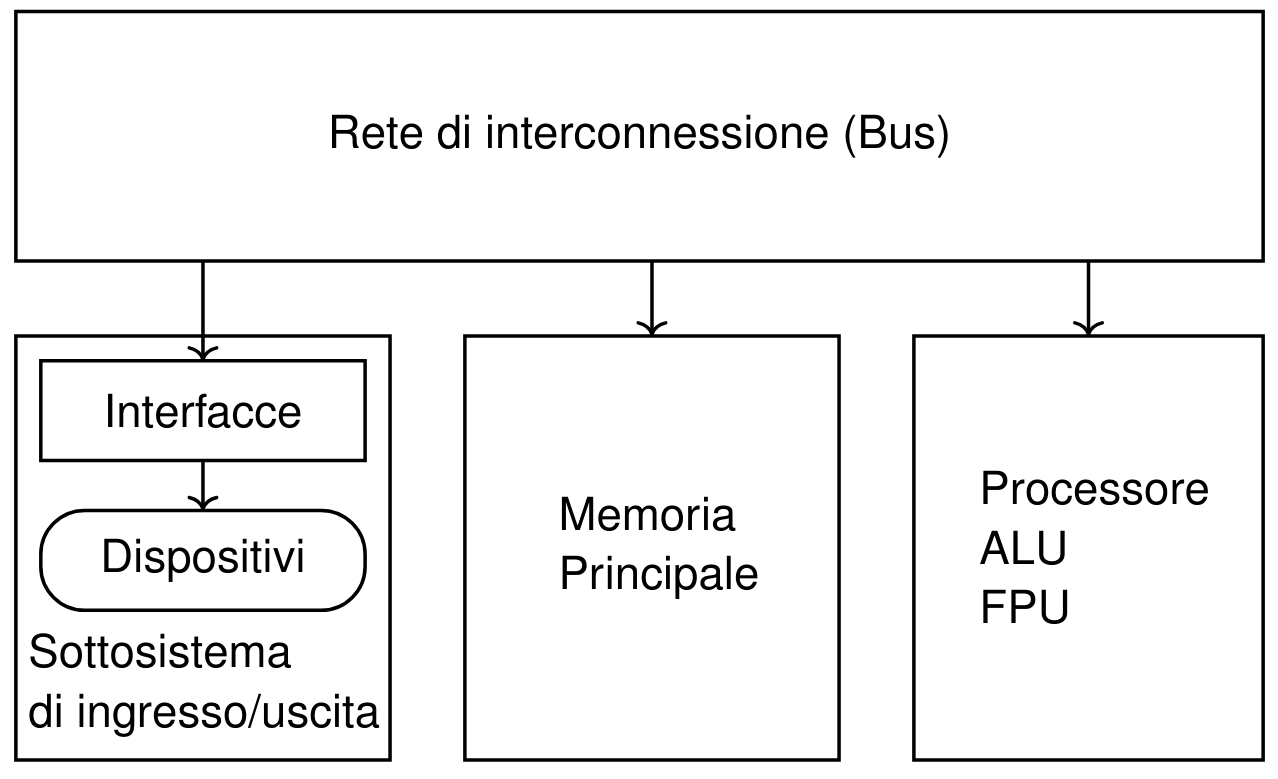
\includegraphics[scale=0.35]{../figures/struttura_calc.png}
\end{center}

Vediamo quindi come questi componenti comunicano fra di loro:
\begin{itemize}
	\item La rete di interconnessione (bus) serve tutti (a scapito della direzione delle frecce, può supportare la comunicazione \textit{da} e \textit{a} componenti);
	\item Il processore e la RAM si trovano sul bus;
	\item I dispositivi, cioè i trasduttori col mondo esterno, comunicano con il sistema attraverso le loro \textit{interfacce}, che obbedisce da un lato alle regole del bus e dall'altro alle specifiche del dispositivo stesso per permettere la comunicazione.
\end{itemize}

\subsection{Interfacce}
Abbiamo visto come fra il calcolatore ed ogni dispositivo si trovi un'apposita \textit{interfaccia}.

Di base, ogni interfaccia è caratterizzata da più registri (accessibili nello spazio di I/O), che possono essere scritti o letti dal calcolatore per dare o ottenere informazioni dal dispositivo.
Notiamo che letture e scritture sui registri delle interfacce possono essere distruttive: spesso il dispositivo implementa particolari funzioni che vengono lanciate da operazioni di questo tipo (un registro che si azzera dopo esser letto, ecc...).

Nel caso più semplice, in ogni caso, un'interfaccia dispone di almeno 3 registri:
\begin{itemize}
	\item Registro di \textbf{stato}, che segnala lo stato corrente dell'interfaccia (se è di uscita può segnalare che è pronta a ricevere dati, se di entrata che ci sono dati pronti, ecc...);
	\item Registro di \textbf{controllo}, che permette al calcolatore di comandarne l'operazione (se di entrata può impedire che nuovi dati arrivino in ingresso, ecc...);
	\item Uno o più \textbf{buffer dati}, resi accessibili attraverso un registro di lettura. Solitamente si dice \textbf{TBR} (\textit{Transfer Buffer Register}) il registro che accede al buffer di uscita e \textbf{RBR} (\textit{Receive Buffer Register}) il registro che accede al buffer di entrata. Nel caso di interfacce di ingresso/uscita TBR e RBR stanno alla stessa porta dello spazio di I/O, e quale viene reso disponibile al processore varia in base al tipo di operazione che esso richiede (TBR per uscita, RBR per ingresso).
\end{itemize}

\subsection{Interruzioni}
Veniamo quindi al meccanismo dell'\textbf{interruzione}.
Nella formulazione originale di Dijkstra queste servivano a risparmiare al processore l'attesa "attiva" (\textit{busy wait}) dei bit di stato delle interfacce, delegando questo invece ad una segnalazione esplicita da parte dell'interfaccia, che viene \textit{gestita} dal processore mettendo in esecuzione un determinato \textit{handler} di interruzione.

Per gestire correttamente le interruzioni abbiamo bisogno di un po' di infrastruttura in più:
\begin{itemize}
	\item Una nuova fase processore, successiva all'esecuzione, che si occupa di controllare le richieste di interruzioni in arrivo (nei sistemi x86 \textit{la} richiesta, che è stata inoltrata da un sottosistema detto APIC);
	\item Una zona di memoria dove viene allocata la \textbf{IVT} (\textit{Interrupt Vector Table}), che associa ad un indice (cioè il tipo di interruzione) l'inizio dell'handler relativo a tale tipo;
	\item Una nuova istruzione, \lstinline|IRET|, che si occupa di ritornare da un gestore di interruzione.

		Non potremmo usare la semplice RET in quanto ogni interruzione salva dello stato aggiuntivo oltre al semplice IP sulla pila: di base, salveremo anche il registro dei FLAG.
\end{itemize}

\subsubsection{Tipi di interruzione}
Abbiamo visto nel corso di calcolatori elettronici come il meccanismo delle interruzioni può essere sfruttato per implementare molta più funzionalità di quelle relative alla gestione dei dispositivi.
In particolare, i calcolatori moderni dispongono di più tipi di interruzioni:
\begin{itemize}
	\item Interruzioni \textbf{esterne}, del tipo che abbiamo appena visto, che si distinguono ulteriormente in:
		\begin{itemize}
			\item Interruzioni esterne \textbf{mascherabili}, cioè che possono essere ignorate variando il flag IF;
			\item Interruzioni esterne \textbf{non mascherabili}, cioè che vengono sempre gestite;
		\end{itemize}
	\item Interruzioni \textbf{interne}, cioè lanciate da situazioni interne al processore (eccezioni);
	\item Interruzioni \textbf{software}, che possono essere lanciate dal programmatore attraverso l'apposita istruzione \lstinline|INT|.
\end{itemize}

\subsection{Meccanismi di protezione}
Veniamo quindi ai meccanismi tipici del S/O in sé per sé.
Se vogliamo la separazione fra processi e S/O che gestisce quei processi (e quindi ha l'accesso prioritario alle risorse di sistema), dobbiamo separare l'operazione del calcolatore in due modalità principali:
\begin{itemize}
	\item Modalità \textbf{utente}: usata per la normale esecuzione dei programmi, non è possibile accedere a tutte le risorse di sistema;
	\item Modalità \textbf{supervisor}: usata per lo svolgimento delle chiamate sistema (primitive), tutte le risorse di sistema sono disponibili.
\end{itemize}

Importante è che il passaggio da modo utente a modo supervisor richieda al programma in esecuzione in modo utente di "abbandonare" il controllo, cedendolo ad una primitiva sistema.
Vedremo come questo si può implementare agilmente sfruttando il meccanismo di interruzione.

\subsection{Componenti del S/O}
Vediamo quindi, come abbiamo fatto per l'hardware, quelli che sono i \textbf{componenti} del S/O e come questi sono organizzati.

Prendiamo come riferimento un sistema \textit{Unix}, in quanto più semplice ed elegante per i nostri scopi.

Adottando un approccio \textit{top-down}, dove per \textit{top} intendiamo lo spazio dell'utente, vediamo le seguenti componenti:
\begin{itemize}
	\item L'\textit{userspace}, cioè gli applicativi utente veri e propri;
	\item Gli strumenti che il S/O fornisce all'utente per la gestione del sistema, cioè:
		\begin{itemize}
			\item La \textbf{shell};
			\item \textbf{Compilatore} e \textbf{linker};
			\item Le \textbf{librerie} sistema (che si rivolgono ad API, ecc...).
		\end{itemize}
	\item Il \textbf{kernel}, cioè la parte del S/O che effettivamente gestisce il sistema. Qui troviamo:
		\begin{itemize}
			\item Il sottosistema \textbf{file}, che gestisce il filesystem su uno o più dispositivi a blocchi;
			\item A sua volta il sottosistema file interagisce con i \textbf{driver} dispositivo (in particolare coi driver dei dispositivi a blocchi), che hanno il compito di gestire a livello hardware il comportamento dei dispositivi;
			\item Inoltre, troviamo il sottosistema \textbf{controllo processi}, composto da:
				\begin{itemize}
					\item Funzionalità \textbf{IPC} (\textit{Inter Process Communication}) per la comunicazione fra processi;
					\item Lo \textbf{scheduler}, che decide quali processi mandare in esecuzione;
					\item Il sottosistema di \textbf{gestione memoria}, che gestisce lo spazio in memoria principale allocato per ogni processo, interagendo col meccanismo della \textit{memoria virtuale}.
				\end{itemize}
		\end{itemize}
	\item Infine, il \textit{kernel} si appoggia all'\textbf{hardware} della macchina. 
\end{itemize}

\subsubsection{Modello gerarchico}
Un modello più complesso per S/O potrebbe elaborare su questa struttura, prevedendo più livelli intermedi di kernel che implementano \textit{macchine virtuali} via via più vicine all'hardware.
Ognuna di queste fornirà al livello superiore funzioni (effettivamente chiamate sistema) sempre più astratte, che implementeranno nel complesso le chiamate sistema rese disponibili ai processi utente.

\subsubsection{Modello client-server}
Un'altro modello possibile per sistemi distribuiti in rete è quello di avere più \textit{nodi} collegati alla stessa rete.
Ogni nodo disporrà del suo kernel, e in esecuzione su quel kernel avrà uno specifico processo (utente o sistema).

La funzionalità del S/O sarà quindi implementata interrogando la rete per il servizio richiesto: sarà quindi compito della macchina su quella rete che effettivamente implementa tale servizio rispondere e fornire, appunto, il servizio.

In ogni caso non analizzeremo sistemi di questo tipo in questo corso, relativi più che altro a sistemi su \textit{cloud}, e quindi all'ambito delle reti informatiche.

\subsection{Gestione processi}
Informalmente, il termine processo viene usato per indicare un programma in esecuzione sulla macchina.

\begin{itemize}
	\item Rappresenta la \textit{sequenza di eventi} generati dall'elaboratore durante l'esecuzione;
	\item Identifica la più piccola \textit{unità di esecuzione} dentro un S/O multiprogrammato: questo consentirà l'esecuzione di \textit{più} processi concorrenti;
\end{itemize}

Un processo va necessariamente \textit{descritto}, cioè bisogna definire un \textbf{descrittore} che lo rappresenta.
Del processo ci interessa:
\begin{itemize}
	\item Il \textbf{codice} del programma che esegue;
	\item I \textbf{dati};
	\item Il valore dell'\textbf{IP};
	\item Lo stato dei \textbf{registri};
	\item Lo \textbf{stack}.
\end{itemize}

Inoltre, ad un certo processo potranno essere associate delle risorse:
\begin{itemize}
	\item \textbf{Memoria} utilizzata;
	\item \textbf{File} aperti;
	\item \textbf{Dispositivi} di I/O a cui ha accesso.
\end{itemize}

\subsubsection{Processi in memoria}
Il processo in memoria ha a disposizione il suo \textit{spazio di indirizzamento virtuale}. 
Viene detto \textit{virtuale} perché verrà allocato in una memoria centrale fisica, le cui locazioni potrebbero non corrispondere esattamente con la memoria offerta al processo (attraverso il meccanismo della \textit{memoria virtuale}).

Partendo dal basso, le regioni di memoria fornite al processo nel suo spazio di indirizzamento saranno:
\begin{enumerate}
	\item \lstinline|text|: contiene il codice del processo;
	\item \lstinline|data|: contiene i dati statici del programa (sezione \lstinline|data| e \lstinline|bss|, che contiene lo spazio riservato a variabili statiche non allocate);
	\item \lstinline|heap|: l'heap del processo, dove vengono allocati oggetti in memoria dinamica; 
	\item \lstinline|stack|: si sviluppa verso il basso, rappresenta la pila del processo in esecuzione.
\end{enumerate}

\end{document}

\documentclass[a4paper,11pt]{article}
\usepackage[a4paper, margin=8em]{geometry}

% usa i pacchetti per la scrittura in italiano
\usepackage[french,italian]{babel}
\usepackage[T1]{fontenc}
\usepackage[utf8]{inputenc}
\frenchspacing 

% usa i pacchetti per la formattazione matematica
\usepackage{amsmath, amssymb, amsthm, amsfonts}

% usa altri pacchetti
\usepackage{gensymb}
\usepackage{hyperref}
\usepackage{standalone}

\usepackage{colortbl}

\usepackage{xstring}
\usepackage{karnaugh-map}

% imposta il titolo
\title{Appunti Sistemi Operativi}
\author{Luca Seggiani}
\date{2025}

% imposta lo stile
% usa helvetica
\usepackage[scaled]{helvet}
% usa palatino
\usepackage{palatino}
% usa un font monospazio guardabile
\usepackage{lmodern}

\renewcommand{\rmdefault}{ppl}
\renewcommand{\sfdefault}{phv}
\renewcommand{\ttdefault}{lmtt}

% circuiti
\usepackage{circuitikz}
\usetikzlibrary{babel}

% testo cerchiato
\newcommand*\circled[1]{\tikz[baseline=(char.base)]{
            \node[shape=circle,draw,inner sep=2pt] (char) {#1};}}

% disponi il titolo
\makeatletter
\renewcommand{\maketitle} {
	\begin{center} 
		\begin{minipage}[t]{.8\textwidth}
			\textsf{\huge\bfseries \@title} 
		\end{minipage}%
		\begin{minipage}[t]{.2\textwidth}
			\raggedleft \vspace{-1.65em}
			\textsf{\small \@author} \vfill
			\textsf{\small \@date}
		\end{minipage}
		\par
	\end{center}

	\thispagestyle{empty}
	\pagestyle{fancy}
}
\makeatother

% disponi teoremi
\usepackage{tcolorbox}
\newtcolorbox[auto counter, number within=section]{theorem}[2][]{%
	colback=blue!10, 
	colframe=blue!40!black, 
	sharp corners=northwest,
	fonttitle=\sffamily\bfseries, 
	title=Teorema~\thetcbcounter: #2, 
	#1
}

% disponi definizioni
\newtcolorbox[auto counter, number within=section]{definition}[2][]{%
	colback=red!10,
	colframe=red!40!black,
	sharp corners=northwest,
	fonttitle=\sffamily\bfseries,
	title=Definizione~\thetcbcounter: #2,
	#1
}

% disponi codice
\usepackage{listings}
\usepackage[table]{xcolor}

\definecolor{codegreen}{rgb}{0,0.6,0}
\definecolor{codegray}{rgb}{0.5,0.5,0.5}
\definecolor{codepurple}{rgb}{0.58,0,0.82}
\definecolor{backcolour}{rgb}{0.95,0.95,0.92}

\lstdefinestyle{codestyle}{
		backgroundcolor=\color{black!5}, 
		commentstyle=\color{codegreen},
		keywordstyle=\bfseries\color{magenta},
		numberstyle=\sffamily\tiny\color{black!60},
		stringstyle=\color{green!50!black},
		basicstyle=\ttfamily\footnotesize,
		breakatwhitespace=false,         
		breaklines=true,                 
		captionpos=b,                    
		keepspaces=true,                 
		numbers=left,                    
		numbersep=5pt,                  
		showspaces=false,                
		showstringspaces=false,
		showtabs=false,                  
		tabsize=2
}

\lstdefinestyle{shellstyle}{
		backgroundcolor=\color{black!5}, 
		basicstyle=\ttfamily\footnotesize\color{black}, 
		commentstyle=\color{black}, 
		keywordstyle=\color{black},
		numberstyle=\color{black!5},
		stringstyle=\color{black}, 
		showspaces=false,
		showstringspaces=false, 
		showtabs=false, 
		tabsize=2, 
		numbers=none, 
		breaklines=true
}


\lstdefinelanguage{assembler}{ 
  keywords={AAA, AAD, AAM, AAS, ADC, ADCB, ADCW, ADCL, ADD, ADDB, ADDW, ADDL, AND, ANDB, ANDW, ANDL,
        ARPL, BOUND, BSF, BSFL, BSFW, BSR, BSRL, BSRW, BSWAP, BT, BTC, BTCB, BTCW, BTCL, BTR, 
        BTRB, BTRW, BTRL, BTS, BTSB, BTSW, BTSL, CALL, CBW, CDQ, CLC, CLD, CLI, CLTS, CMC, CMP,
        CMPB, CMPW, CMPL, CMPS, CMPSB, CMPSD, CMPSW, CMPXCHG, CMPXCHGB, CMPXCHGW, CMPXCHGL,
        CMPXCHG8B, CPUID, CWDE, DAA, DAS, DEC, DECB, DECW, DECL, DIV, DIVB, DIVW, DIVL, ENTER,
        HLT, IDIV, IDIVB, IDIVW, IDIVL, IMUL, IMULB, IMULW, IMULL, IN, INB, INW, INL, INC, INCB,
        INCW, INCL, INS, INSB, INSD, INSW, INT, INT3, INTO, INVD, INVLPG, IRET, IRETD, JA, JAE,
        JB, JBE, JC, JCXZ, JE, JECXZ, JG, JGE, JL, JLE, JMP, JNA, JNAE, JNB, JNBE, JNC, JNE, JNG,
        JNGE, JNL, JNLE, JNO, JNP, JNS, JNZ, JO, JP, JPE, JPO, JS, JZ, LAHF, LAR, LCALL, LDS,
        LEA, LEAVE, LES, LFS, LGDT, LGS, LIDT, LMSW, LOCK, LODSB, LODSD, LODSW, LOOP, LOOPE,
        LOOPNE, LSL, LSS, LTR, MOV, MOVB, MOVW, MOVL, MOVSB, MOVSD, MOVSW, MOVSX, MOVSXB,
        MOVSXW, MOVSXL, MOVZX, MOVZXB, MOVZXW, MOVZXL, MUL, MULB, MULW, MULL, NEG, NEGB, NEGW,
        NEGL, NOP, NOT, NOTB, NOTW, NOTL, OR, ORB, ORW, ORL, OUT, OUTB, OUTW, OUTL, OUTSB, OUTSD,
        OUTSW, POP, POPL, POPW, POPB, POPA, POPAD, POPF, POPFD, PUSH, PUSHL, PUSHW, PUSHB, PUSHA, 
				PUSHAD, PUSHF, PUSHFD, RCL, RCLB, RCLW, MOVSL, MOVSB, MOVSW, STOSL, STOSB, STOSW, LODSB, LODSW,
				LODSL, INSB, INSW, INSL, OUTSB, OUTSL, OUTSW
        RCLL, RCR, RCRB, RCRW, RCRL, RDMSR, RDPMC, RDTSC, REP, REPE, REPNE, RET, ROL, ROLB, ROLW,
        ROLL, ROR, RORB, RORW, RORL, SAHF, SAL, SALB, SALW, SALL, SAR, SARB, SARW, SARL, SBB,
        SBBB, SBBW, SBBL, SCASB, SCASD, SCASW, SETA, SETAE, SETB, SETBE, SETC, SETE, SETG, SETGE,
        SETL, SETLE, SETNA, SETNAE, SETNB, SETNBE, SETNC, SETNE, SETNG, SETNGE, SETNL, SETNLE,
        SETNO, SETNP, SETNS, SETNZ, SETO, SETP, SETPE, SETPO, SETS, SETZ, SGDT, SHL, SHLB, SHLW,
        SHLL, SHLD, SHR, SHRB, SHRW, SHRL, SHRD, SIDT, SLDT, SMSW, STC, STD, STI, STOSB, STOSD,
        STOSW, STR, SUB, SUBB, SUBW, SUBL, TEST, TESTB, TESTW, TESTL, VERR, VERW, WAIT, WBINVD,
        XADD, XADDB, XADDW, XADDL, XCHG, XCHGB, XCHGW, XCHGL, XLAT, XLATB, XOR, XORB, XORW, XORL},
  keywordstyle=\color{blue}\bfseries,
  ndkeywordstyle=\color{darkgray}\bfseries,
  identifierstyle=\color{black},
  sensitive=false,
  comment=[l]{\#},
  morecomment=[s]{/*}{*/},
  commentstyle=\color{purple}\ttfamily,
  stringstyle=\color{red}\ttfamily,
  morestring=[b]',
  morestring=[b]"
}

\lstset{language=assembler, style=codestyle}

% disponi sezioni
\usepackage{titlesec}

\titleformat{\section}
	{\sffamily\Large\bfseries} 
	{\thesection}{1em}{} 
\titleformat{\subsection}
	{\sffamily\large\bfseries}   
	{\thesubsection}{1em}{} 
\titleformat{\subsubsection}
	{\sffamily\normalsize\bfseries} 
	{\thesubsubsection}{1em}{}

% tikz
\usepackage{tikz}

% float
\usepackage{float}

% grafici
\usepackage{pgfplots}
\pgfplotsset{width=10cm,compat=1.9}

% disponi alberi
\usepackage{forest}

\forestset{
	rectstyle/.style={
		for tree={rectangle,draw,font=\large\sffamily}
	},
	roundstyle/.style={
		for tree={circle,draw,font=\large}
	}
}

% disponi algoritmi
\usepackage{algorithm}
\usepackage{algorithmic}
\makeatletter
\renewcommand{\ALG@name}{Algoritmo}
\makeatother

% disponi numeri di pagina
\usepackage{fancyhdr}
\fancyhf{} 
\fancyfoot[L]{\sffamily{\thepage}}

\makeatletter
\fancyhead[L]{\raisebox{1ex}[0pt][0pt]{\sffamily{\@title \ \@date}}} 
\fancyhead[R]{\raisebox{1ex}[0pt][0pt]{\sffamily{\@author}}}
\makeatother

\begin{document}
% sezione (data)
\section{Lezione del 02-10-25}

% stili pagina
\thispagestyle{empty}
\pagestyle{fancy}

% testo
Continuiamo la discussione dei processi:

\subsubsection{Stato dei processi}
In un \textbf{S/O monoprogrammato} il processo può trovarsi in uno di due stati:

\begin{center}
	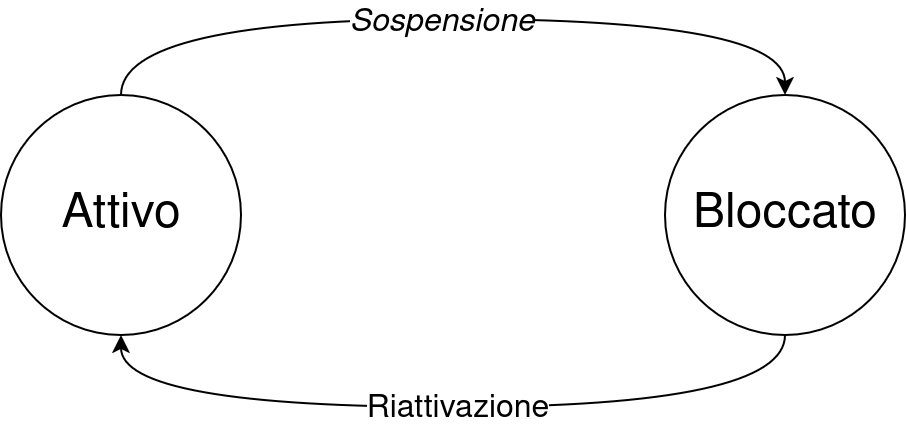
\includegraphics[scale=0.25]{../figures/proc_attivo_bloccato.png}
\end{center}

\begin{itemize}
	\item \textbf{Attivo}: il processo stato creato, è in esecuzione ed ha ancora istruzioni da eseguire. 

		\textit{Creare} un processo significa in primo luogo allocare le strutture dati che lo descrivono. In seguito, si deve allocare un po' di memoria al processo stesso per contenere i suoi dati (istruzioni, pila, ecc...) come visto in 4.6.
	Abbiamo però che allocare particolari descrittori al processo quando questo è l'unico in esecuzione sarebbe inutile: effettivamente un sistema monoprogrammato può essere tale solo se il processo in esecuzione è in qualche modo il S/O.

		A questo punto il processo è l'unico in esecuzione sulla CPU, e resterà tale fino alla fine del suo \textit{lifetime}.
		Dovrà però \textit{bloccarsi} se vuole accedere a risorse sistema: fara ciò usando una \textit{chiamata a sistema};

	\item \textbf{Bloccato}: il processo o qualche altro attore ha causato un qualche evento che ha determinato il passaggio di controllo al S/O (richiesta risorse di I/O, di risorse logiche, interruzioni esterne, ecc...).

		A questo punto sarà nuovamente un evento esterno (interruzione esterna, azione dell'utente) a riportare in esecuzione un processo, creandone uno nuovo se lo scorso aveva terminato, o rimettendo il corrente in esecuzione se si era bloccao su una operazione di I/O o simile.

		Notiamo che la memoria del processo potrebbe cambiare anche questo è bloccato: ad esempio se si hanno dispositivi che operano in DMA. 
\end{itemize}

La transizione fra attivo e bloccato è detta \textit{sospensione}, mentre fra bloccato e attivo è è detta \textit{riattivazione}.

Possiamo dire che gli stati \textit{attivo} e \textit{bloccato} sono in qualche modo in corrispondenza con le fasi descritte in 2.1.4 di \textbf{CPU-Burst} e \textbf{I/O-Burst}.

\par\bigskip

Se il numero di CPU è minore del numero dei processi, cioè in un sistema \textbf{monoprocessore}, ci dotiamo di più stati:

\begin{center}
	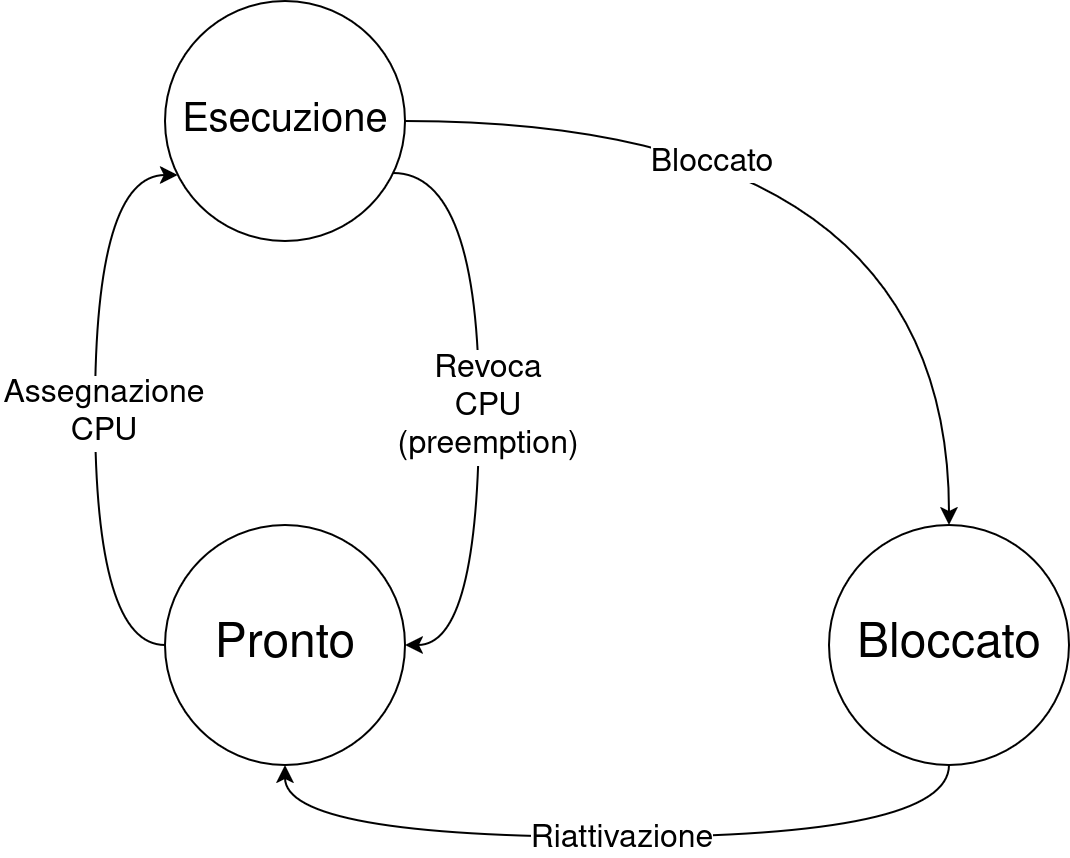
\includegraphics[scale=0.25]{../figures/proc_esecuzione_pronto_bloccato.png}
\end{center}

\begin{itemize}
	\item \textbf{Pronto}: in questo caso il processo è in attesa del tempo del processore. Abbiamo che nella maggior parte delle implementazioni questo stato è rappresentato da una \textit{coda} di descrittori di processo, la cosiddetta \textbf{coda pronti} (utile per implementare politiche prioritarie $\leftrightarrow$ code prioritarie);
	\item \textbf{Esecuzione}: il processo è in esecuzione sulla CPU;
	\item \textbf{Bloccato}: il processo è in attesa, come nell'esempio precedente. 

		In questo caso, come nel precedente, la memoria processo potrebbe essere modificata da dispositivi in DMA.
	Potrebbero poi essere modificati, in particolari situazioni, i descrittori di processo: magari a causa di operazioni di altri processi col S/O (pipe fra processi, ecc...).	
\end{itemize}

La transizione da pronto e esecuzione è detta \textit{assegnazione CPU}, mentre la contraria è detta \textit{revoca CPU}, o in inglese \textbf{preemption}.
Notiamo che quest'ultima transizione non è prevista da tutti i sistemi.

L'operazione di assegnazione CPU è eseguita da un componente del S/O detto \textbf{scheduler}. Lo scheduler viene eseguito quando il processo in esecuzione cambia stato, quindi in caso di \textit{revoca CPU} o \textit{sospensione}: sostanzialmente ogni volta che si richiede un nuovo processo da mettere in esecuzione.
Questo comprende anche la situazione in cui il processo corrente \textit{termina}.

Abbiamo poi che la transizioni allo stato bloccato sono le stesse dell'esempio precedente, con l'unica differenza che la \textit{riattivazione} del processo non lo mette in esecuzione ma nello stato \textit{pronto}.

C'è inoltre un'altro stato, oltre a quello di \textit{terminazione} prima accennato, di cui dobbiamo tener conto: quello in cui il processo viene \textit{creato}, cioè la transizione di un nuovo processo allo stato di \textit{pronto} (detta \textit{attivazione}):

\begin{center}
	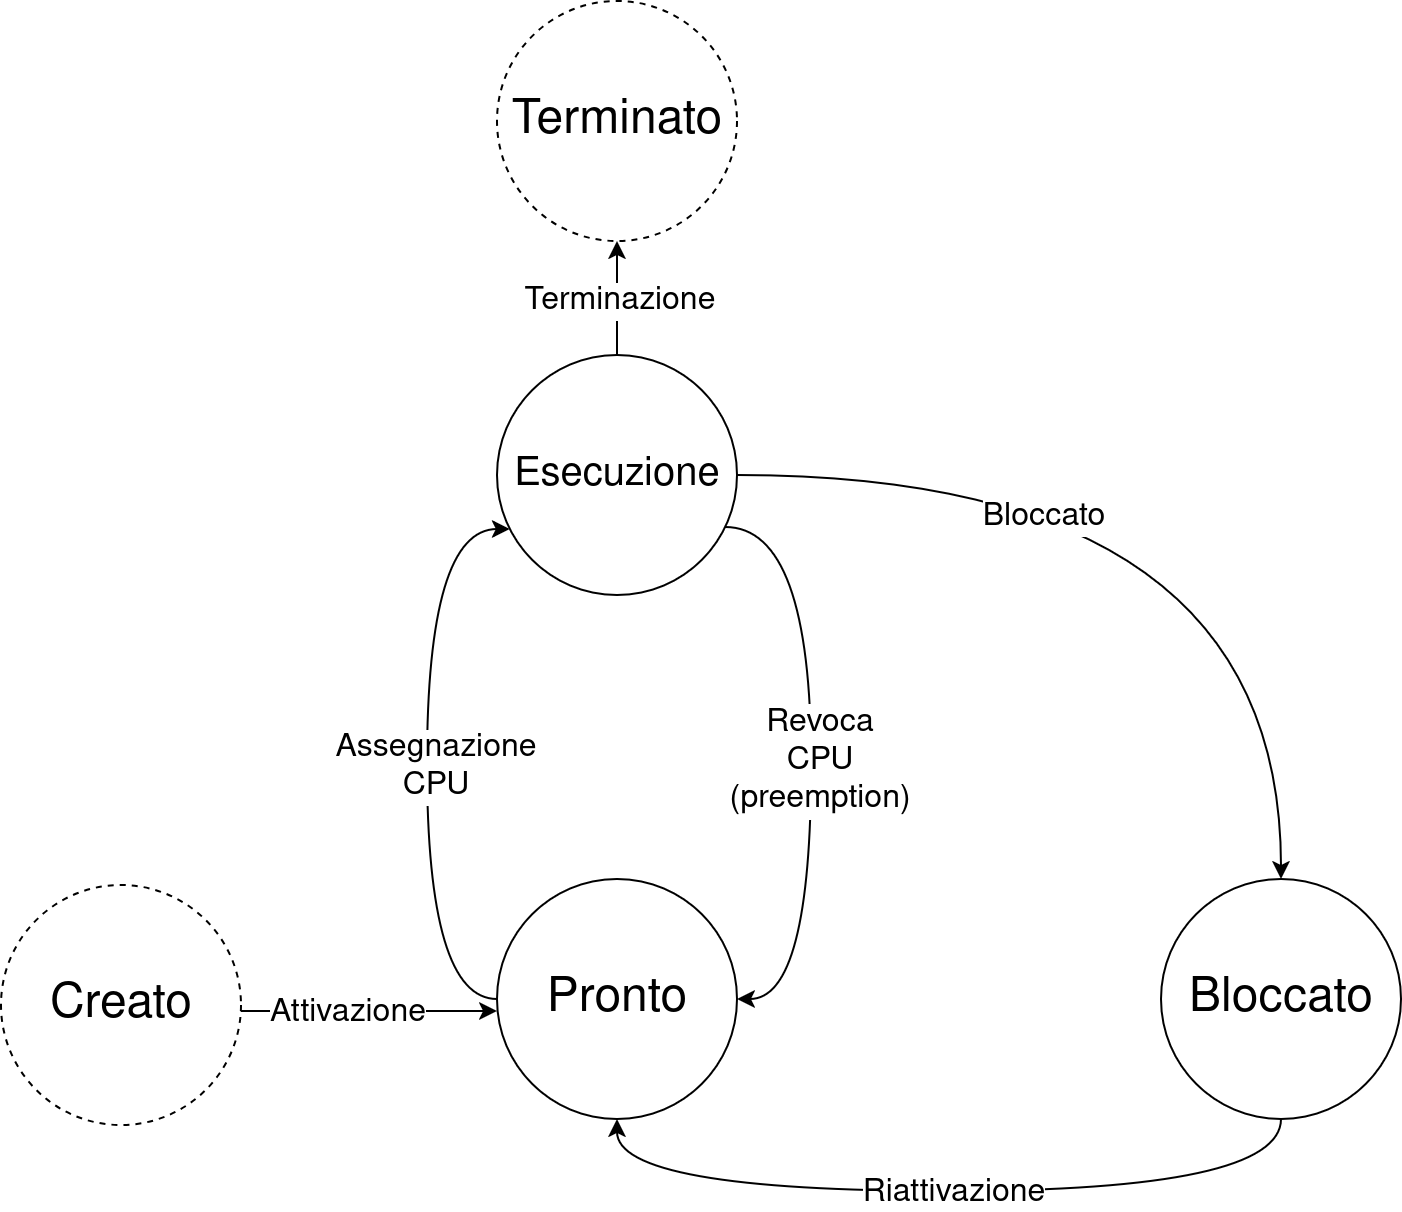
\includegraphics[scale=0.25]{../figures/proc_creato_esecuzione_pronto_bloccato_terminato.png}
\end{center}

In questo caso possiamo anticipare che in S/O che adottano politiche \textit{prioritarie} allo scheduling potrebbe essere necessario eseguire lo scheduler (per mettere in esecuzione un nuovo processo di priorità più alta).

\subsubsection{Descrittori di processo}
Abbiamo introdotto come la gestione dei processi bisogna di apposite strutture dati dette \textit{descrittori} di processo (in inglese \textbf{PCB}, \textit{Process Control Block}).

Questa dovrà associare ad ogni processo:
\begin{itemize}
	\item Nome del processo: questo è il solito \textbf{PID} (\textit{Process IDentifier}), ed identifica univocamente ogni processo. Richiedere che i PID siano univici è una \textit{politica} che li trasforma in una \textit{risorsa}: l'S/O dovrà impegnarsi a gestire i PID in modo che non avvengano collisioni;
	\item Stato del processo: codifica uno degli stati definiti prima;
	\item Modalità di servizio: questo riguarda la priorità (se implementata) o il tipo di scheduling che si usa per gestire il processo;
	\item Informazioni sulla gestione della memoria: conterrà puntatori alla memoria dedicata al processo;
	\item Contesto del processo: l'immagine dei registri all'ultima sospensione del processo;
	\item Utilizzo delle risorse: conterrà puntatori alle risorse logiche e fisiche a cui ha accesso il processo;
	\item Idefntificazione del processo successivo: questo serve semplicemente ad implementare, come abbiamo accennato, le code prioritarie di processi (come ad esempio la \textit{coda pronti}).
\end{itemize}

Una volta definito il descrittore di processo, potremo volerci fornire di:
\begin{itemize}
	\item La coda dei processi pronti;
	\item Una o più code per i processi bloccati (solitamente una coda è associata a una risorsa su cui i processi si bloccano);
	\item Un registro di qualche tipo che contiene il processo attualmente in esecuzione. 
\end{itemize}

\subsubsection{Cambio di contesto}
Il \textbf{cambio di contesto} è l'operazione attraverso cui l'uso del processore viene commutato da un processo all'altro.
Questo consiste in:
\begin{itemize}
	\item Salvataggio del contesto del processo in esecuzione nel suo descrittore (cioè salvataggio di \textit{stato});
	\item Inserimento del descrittore di processo corrente in coda \textit{bloccati} o \textit{pronti}.
	\item Selezione di un nuovo processo da mettere in esecuzione e caricamento nel registro del descrittore del processo corrente (\textit{short term schedulilng});
	\item Caricamento del contesto del nuovo processo e cessione a questi del controllo. 
\end{itemize}

Notiamo che per realizzare il cambio di contesto al S/O (che si occupa poi di portare avanti queste operazioni) abbiamo bisogno di funzionalità implementate in hardware: il "processo" S/O è semplicemente il processo in esecuzione al tempo del cambio, che è forzato a passare al contesto sistema nell'istante in cui si mette ad eseguire codice sistema.

Questo significa che per realizzare un S/O si necessita di un processore che implementi il cambio di contesto (x86 dal 286, ecc...). 

\par\smallskip

Possiamo iniziare ad approfondire il modo in cui indicizziamo il processo. Dal punto di vista concettuale, vorremo usare una tripla:
$$
S = < \text{PID}, \text{UID}, \text{GID} >
$$
composta da \textbf{PID} (\textit{Process IDentifier}, già visto), e \textbf{UID} e \textbf{GID} (\textit{User IDentifier} e \textit{Group IDentifier}), che rappresentano il proprietario del processo.

In caso di cambi di contesto al contesto sistema, quello che faremo è semplicemente cambiare UID e GID in modo da eseguire lo stesso processo, ma con privilegi diversi.

\subsubsection{Creazione e terminazione di processi}
Vediamo le operazioni che si possono svolgere sui processi.

Avremo che vorremo supportare \textit{gerarchie} di procssi, dove un processo (padre) può richiedere la creazione di un nuovo processo (figlio).
Questo significherà che ogni processo sarà figlio di un altro processa, e potra a sua volta essere padre di altri processi.
Chiaramente, le informazioni relative alle relazioni parentali saranno mantenute da S/O nei descrittori di processi.

Se un processo termina, di base:
\begin{itemize}
	\item Il padre può rilevare il suo stato di terminazione;
	\item Tutti i suoi figli terminano.
\end{itemize}

\subsubsection{Processi concorrenti}
Specifichiamo come più processi vengono eseguiti su una stessa macchina.
Abbiamo che questi possono alternarsi (\textit{interleaving}), tipico delle macchine a singolo processore, o eseguire effettivamente l'uno contemporaneamente all'altro. Questo è tipico delle macchine a più processori.

Nel caso di più processi in esecuzione contemporaneamente (diciamo processi \textit{concorrenti}) vengono a verificarsi alcune problematiche:
\begin{itemize}
	\item Processi \textbf{indipendenti}: se due processi $P1$ e $P2$ sono indipendenti, cioè non influenzano l'uno l'esecuzione dell'altra, dobbiamo assicurarci che questo resti vero, cioè dobbiamo risolvere il \textit{problema della riproducibilità}. Visto che le risorse sistema sono condivise, dobbiamo infatti assicurarci che non ci siano effetti collaterali sensibili da un processo o dall'altro.
	\item Processi \textbf{interagenti}: se due processi $P1$ e $P2$ devono interagire fra di loro, possono farlo in maniera \textit{esplicita} (per \textbf{cooperazione}), scambiandosi messaggi, o \textit{implicita} (per \textbf{competizione}), magari competendo per la stessa risorsa in mutua esclusione.
\end{itemize}


\end{document}

\documentclass[a4paper,11pt]{article}
\usepackage[a4paper, margin=8em]{geometry}

% usa i pacchetti per la scrittura in italiano
\usepackage[french,italian]{babel}
\usepackage[T1]{fontenc}
\usepackage[utf8]{inputenc}
\frenchspacing 

% usa i pacchetti per la formattazione matematica
\usepackage{amsmath, amssymb, amsthm, amsfonts}

% usa altri pacchetti
\usepackage{gensymb}
\usepackage{hyperref}
\usepackage{standalone}

\usepackage{colortbl}

\usepackage{xstring}
\usepackage{karnaugh-map}

% imposta il titolo
\title{Appunti Sistemi Operativi}
\author{Luca Seggiani}
\date{2025}

% imposta lo stile
% usa helvetica
\usepackage[scaled]{helvet}
% usa palatino
\usepackage{palatino}
% usa un font monospazio guardabile
\usepackage{lmodern}

\renewcommand{\rmdefault}{ppl}
\renewcommand{\sfdefault}{phv}
\renewcommand{\ttdefault}{lmtt}

% circuiti
\usepackage{circuitikz}
\usetikzlibrary{babel}

% testo cerchiato
\newcommand*\circled[1]{\tikz[baseline=(char.base)]{
            \node[shape=circle,draw,inner sep=2pt] (char) {#1};}}

% disponi il titolo
\makeatletter
\renewcommand{\maketitle} {
	\begin{center} 
		\begin{minipage}[t]{.8\textwidth}
			\textsf{\huge\bfseries \@title} 
		\end{minipage}%
		\begin{minipage}[t]{.2\textwidth}
			\raggedleft \vspace{-1.65em}
			\textsf{\small \@author} \vfill
			\textsf{\small \@date}
		\end{minipage}
		\par
	\end{center}

	\thispagestyle{empty}
	\pagestyle{fancy}
}
\makeatother

% disponi teoremi
\usepackage{tcolorbox}
\newtcolorbox[auto counter, number within=section]{theorem}[2][]{%
	colback=blue!10, 
	colframe=blue!40!black, 
	sharp corners=northwest,
	fonttitle=\sffamily\bfseries, 
	title=Teorema~\thetcbcounter: #2, 
	#1
}

% disponi definizioni
\newtcolorbox[auto counter, number within=section]{definition}[2][]{%
	colback=red!10,
	colframe=red!40!black,
	sharp corners=northwest,
	fonttitle=\sffamily\bfseries,
	title=Definizione~\thetcbcounter: #2,
	#1
}

% disponi codice
\usepackage{listings}
\usepackage[table]{xcolor}

\definecolor{codegreen}{rgb}{0,0.6,0}
\definecolor{codegray}{rgb}{0.5,0.5,0.5}
\definecolor{codepurple}{rgb}{0.58,0,0.82}
\definecolor{backcolour}{rgb}{0.95,0.95,0.92}

\lstdefinestyle{codestyle}{
		backgroundcolor=\color{black!5}, 
		commentstyle=\color{codegreen},
		keywordstyle=\bfseries\color{magenta},
		numberstyle=\sffamily\tiny\color{black!60},
		stringstyle=\color{green!50!black},
		basicstyle=\ttfamily\footnotesize,
		breakatwhitespace=false,         
		breaklines=true,                 
		captionpos=b,                    
		keepspaces=true,                 
		numbers=left,                    
		numbersep=5pt,                  
		showspaces=false,                
		showstringspaces=false,
		showtabs=false,                  
		tabsize=2
}

\lstdefinestyle{shellstyle}{
		backgroundcolor=\color{black!5}, 
		basicstyle=\ttfamily\footnotesize\color{black}, 
		commentstyle=\color{black}, 
		keywordstyle=\color{black},
		numberstyle=\color{black!5},
		stringstyle=\color{black}, 
		showspaces=false,
		showstringspaces=false, 
		showtabs=false, 
		tabsize=2, 
		numbers=none, 
		breaklines=true
}


\lstdefinelanguage{assembler}{ 
  keywords={AAA, AAD, AAM, AAS, ADC, ADCB, ADCW, ADCL, ADD, ADDB, ADDW, ADDL, AND, ANDB, ANDW, ANDL,
        ARPL, BOUND, BSF, BSFL, BSFW, BSR, BSRL, BSRW, BSWAP, BT, BTC, BTCB, BTCW, BTCL, BTR, 
        BTRB, BTRW, BTRL, BTS, BTSB, BTSW, BTSL, CALL, CBW, CDQ, CLC, CLD, CLI, CLTS, CMC, CMP,
        CMPB, CMPW, CMPL, CMPS, CMPSB, CMPSD, CMPSW, CMPXCHG, CMPXCHGB, CMPXCHGW, CMPXCHGL,
        CMPXCHG8B, CPUID, CWDE, DAA, DAS, DEC, DECB, DECW, DECL, DIV, DIVB, DIVW, DIVL, ENTER,
        HLT, IDIV, IDIVB, IDIVW, IDIVL, IMUL, IMULB, IMULW, IMULL, IN, INB, INW, INL, INC, INCB,
        INCW, INCL, INS, INSB, INSD, INSW, INT, INT3, INTO, INVD, INVLPG, IRET, IRETD, JA, JAE,
        JB, JBE, JC, JCXZ, JE, JECXZ, JG, JGE, JL, JLE, JMP, JNA, JNAE, JNB, JNBE, JNC, JNE, JNG,
        JNGE, JNL, JNLE, JNO, JNP, JNS, JNZ, JO, JP, JPE, JPO, JS, JZ, LAHF, LAR, LCALL, LDS,
        LEA, LEAVE, LES, LFS, LGDT, LGS, LIDT, LMSW, LOCK, LODSB, LODSD, LODSW, LOOP, LOOPE,
        LOOPNE, LSL, LSS, LTR, MOV, MOVB, MOVW, MOVL, MOVSB, MOVSD, MOVSW, MOVSX, MOVSXB,
        MOVSXW, MOVSXL, MOVZX, MOVZXB, MOVZXW, MOVZXL, MUL, MULB, MULW, MULL, NEG, NEGB, NEGW,
        NEGL, NOP, NOT, NOTB, NOTW, NOTL, OR, ORB, ORW, ORL, OUT, OUTB, OUTW, OUTL, OUTSB, OUTSD,
        OUTSW, POP, POPL, POPW, POPB, POPA, POPAD, POPF, POPFD, PUSH, PUSHL, PUSHW, PUSHB, PUSHA, 
				PUSHAD, PUSHF, PUSHFD, RCL, RCLB, RCLW, MOVSL, MOVSB, MOVSW, STOSL, STOSB, STOSW, LODSB, LODSW,
				LODSL, INSB, INSW, INSL, OUTSB, OUTSL, OUTSW
        RCLL, RCR, RCRB, RCRW, RCRL, RDMSR, RDPMC, RDTSC, REP, REPE, REPNE, RET, ROL, ROLB, ROLW,
        ROLL, ROR, RORB, RORW, RORL, SAHF, SAL, SALB, SALW, SALL, SAR, SARB, SARW, SARL, SBB,
        SBBB, SBBW, SBBL, SCASB, SCASD, SCASW, SETA, SETAE, SETB, SETBE, SETC, SETE, SETG, SETGE,
        SETL, SETLE, SETNA, SETNAE, SETNB, SETNBE, SETNC, SETNE, SETNG, SETNGE, SETNL, SETNLE,
        SETNO, SETNP, SETNS, SETNZ, SETO, SETP, SETPE, SETPO, SETS, SETZ, SGDT, SHL, SHLB, SHLW,
        SHLL, SHLD, SHR, SHRB, SHRW, SHRL, SHRD, SIDT, SLDT, SMSW, STC, STD, STI, STOSB, STOSD,
        STOSW, STR, SUB, SUBB, SUBW, SUBL, TEST, TESTB, TESTW, TESTL, VERR, VERW, WAIT, WBINVD,
        XADD, XADDB, XADDW, XADDL, XCHG, XCHGB, XCHGW, XCHGL, XLAT, XLATB, XOR, XORB, XORW, XORL},
  keywordstyle=\color{blue}\bfseries,
  ndkeywordstyle=\color{darkgray}\bfseries,
  identifierstyle=\color{black},
  sensitive=false,
  comment=[l]{\#},
  morecomment=[s]{/*}{*/},
  commentstyle=\color{purple}\ttfamily,
  stringstyle=\color{red}\ttfamily,
  morestring=[b]',
  morestring=[b]"
}

\lstset{language=assembler, style=codestyle}

% disponi sezioni
\usepackage{titlesec}

\titleformat{\section}
	{\sffamily\Large\bfseries} 
	{\thesection}{1em}{} 
\titleformat{\subsection}
	{\sffamily\large\bfseries}   
	{\thesubsection}{1em}{} 
\titleformat{\subsubsection}
	{\sffamily\normalsize\bfseries} 
	{\thesubsubsection}{1em}{}

% tikz
\usepackage{tikz}

% float
\usepackage{float}

% grafici
\usepackage{pgfplots}
\pgfplotsset{width=10cm,compat=1.9}

% disponi alberi
\usepackage{forest}

\forestset{
	rectstyle/.style={
		for tree={rectangle,draw,font=\large\sffamily}
	},
	roundstyle/.style={
		for tree={circle,draw,font=\large}
	}
}

% disponi algoritmi
\usepackage{algorithm}
\usepackage{algorithmic}
\makeatletter
\renewcommand{\ALG@name}{Algoritmo}
\makeatother

% disponi numeri di pagina
\usepackage{fancyhdr}
\fancyhf{} 
\fancyfoot[L]{\sffamily{\thepage}}

\makeatletter
\fancyhead[L]{\raisebox{1ex}[0pt][0pt]{\sffamily{\@title \ \@date}}} 
\fancyhead[R]{\raisebox{1ex}[0pt][0pt]{\sffamily{\@author}}}
\makeatother

\begin{document}
% sezione (data)
\section{Lezione del 07-10-25}

% stili pagina
\thispagestyle{empty}
\pagestyle{fancy}

% testo
\subsection{Nucleo}
Il \textbf{nucleo} o \textit{kernel} è il cuore di un S/O, il componente che ha il compito di realizzare l'astrazione della \textit{CPU virtuale}. Nel caso di sistemi monoprocessore, vogliamo dividere il tempo fra i processi per dargli l'illusione di essere gli unici in esecuzione sulla macchina.

\subsubsection{Scheduling}
Lo scheduling è l'attività secondo la quale il sistema operativo effettua delle scelte fra quali processi caricare in memoria centrale e a quali assegnare la CPU.

Ci sono 3 diverse attività di scheduling:
\begin{itemize}
	\item \textbf{Breve} termine: lo scheduling propriamente detto, il processo attraverso cui si assegna la CPU. Può essere \textit{preemptive} e \textit{non preemptive} (con o senza diritto di revoca). Solitamente viene invocato molto frequentemente (millisecondi);
	\item \textbf{Medio} termine (\textit{swapping}): il trasferimento temporaneo in memoria secondaria dei processi. Si usa quando la memoria centrale dispone di memoria minore della somma di quella richiesta dai vari processi. Viene invocato più di rado (secondi, minuti);
	\item \textbf{Lungo} termine: la scelta di quali processi caricare dalla memoria secondaria in memoria centrale. Rappresenta un componente importante dei sistemi \textit{batch} multiprogrammati, oggi come oggi quindi sui \textit{server} e meno sulle macchine personali;
\end{itemize}

Vediamo quindi una schematica che mostra dove queste attività di scheduling avvengono nell'architettura vista:
\begin{center}
	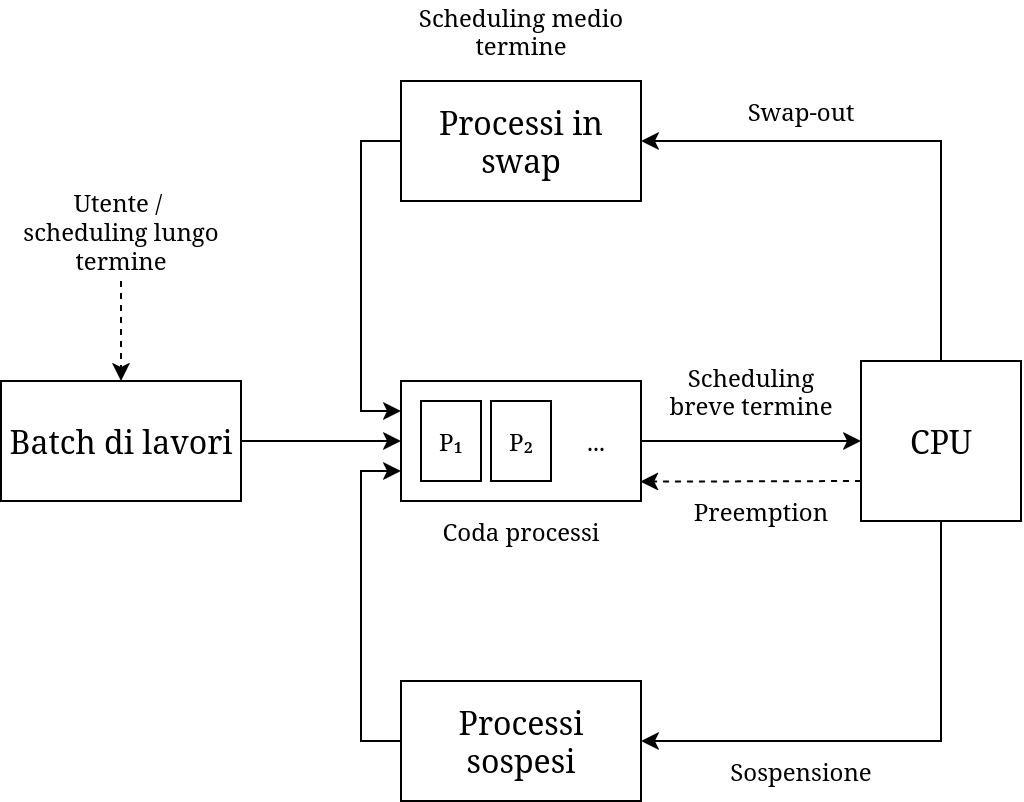
\includegraphics[scale=0.3]{../figures/scheduling.png}
\end{center}

I processi possono in genere classificarsi in:
\begin{itemize}
	\item Processi vincolati da \textbf{I/O}: passano più tempo a fare I/O burst piuttosto che CPU burst (che sono tanti e piccoli);
	\item Processi vincolati da \textbf{CPU}: passano più tempo a fare calcoli, hanno pochi e lunghi CPU burst.
\end{itemize}

\subsection{Algoritmi di scheduling}
Gli algoritmi di scheduling che vedremo saranno:
\begin{itemize}
	\item \textbf{FCFS} (\textit{First Come First Served}): è \textit{non prioritario} e \textit{non preemptive}, consiste nel assegnare la CPU sempre al primo processo arrivato;
	\item \textbf{SJF} (\textit{Shortest Job First}): è \textit{prioritario} e \textit{non preemptive}, consiste nell'assegnare la CPU al processo più breve;
	\item \textbf{SRTF} (\textit{Shortest Remaining Time First}): è \textit{prioritario} e \textit{preemptive}, rappresenta sostanzialmente la versione con revoca del precedente;
	\item \textbf{RR} (\textit{Round Robin}): è \textit{non prioritario} e \textit{preemptive}: si basa sull'assegnare quanti temporali ugualmente ad ogni processo;
	\item Schedulazione \textbf{su base prioritaria}: introdurremo qui l'idea di \textit{priorità} per ogni processo;
	\item Schedulazione \textbf{a code multiple}: prevediamo più code, che possiamo distinguere usando gli algoritmi sopra descritti, o come vedremo sarà conveniente, assegnando una \textit{priorità} ad ogni cosa;
	\item Schedulazione di sistemi \textbf{in tempo reale}. Questi sono algoritmi che devono assicurare la terminazione deterministicad ei processi. In questo vedremo gli algoritmi:
		\begin{itemize}
			\item \textbf{RM} (\textit{Rate Monotonic});
			\item \textbf{EDF} (\textit{Earliest Deadline First}).
		\end{itemize}
\end{itemize}

\subsubsection{Valutazione degli algoritmi di scheduling}
Iniziamo a vedere alcune metriche per la valutazione degli algoritmi di scheduling:

\begin{center}
	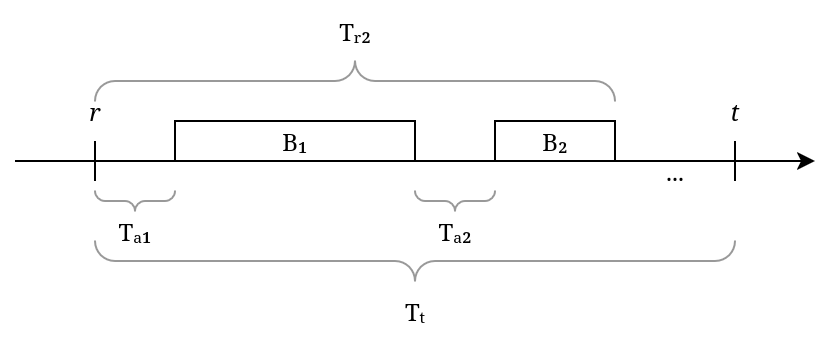
\includegraphics[scale=0.4]{../figures/scheduling_valuta.png}
\end{center}

\begin{itemize}
	\item \textbf{Utilizzazione} della CPU o \textit{efficienza}, cioè definito $\Delta B_i$ il tempo di burst e $T$ il quanto di tempo totale, vogliamo un efficienza $E$:
		$$
			E = \frac{\sum \Delta B_i}{T} < 1
		$$
		il più possibile vicina a 1;
	\item Tempo medio di \textbf{completamento} (o tempo di \textit{turnaround}), cioè il tempo che passa prima che il processo possa completare la sua operazione (terminando). Prendiamo l'istante in cui il processo entra in coda pronti come $r$ (da \textit{richiesto}) e quello in cui termina termina come $t$ (da \textit{termina}). Il tempo di completamento $T_t$ sarà ovviamente:
		$$
			T_t = t - r
		$$
	\item \textbf{Produttività} (o frequenza di \textit{througput}), definita come il numero medio di processi completati nell'unità di tempo, cioè l'inverso del tempo medio di completamento:
		$$
			P = \frac{1}{T_t}
		$$
	\item Tempo di \textbf{risposta}, valutato dall'istante in cui un processo entra in coda pronti $r$ all'istante in cui risponde, cioè termina un CPU burst (solitamente il primo). Purtroppo, non tutto il tempo di completamento $T_c$ è dedicato al processo, ma questo viene eseguito, come sappiamo, in più burst (diciamo $B_1$, $B_2$, ...). Il tempo di turnaround $T_t$ sarà allora il tempo trascorso fra $r$ e la fine di un burst $B_i$, cioè:
		$$
			{T_r}_i = \text{end}(B_i) - r
		$$
	\item Tempo di \textbf{attesa}, cioè la somma dei tempi di attesa posti fra i vari burst:
		$$
		T_a = \sum {t_\alpha}_i
		$$
		Con riferimento ai sistemi interattivi, spesso ci interessa il tempo di attesa iniziale, cioè quello fra l'inserimento in coda pronti e l'inizio del primo CPU burst, o in relazione al nostro schema:
		$$
		T_a' = {t_\alpha}_1 = r - \text{begin}(B_1)
		$$

		Dovrebbe essere chiaro che il tempo di \textit{attesa} si distingue dal tempo di \textit{risposta}, in quanto:
		\begin{itemize}
			\item Il tempo di attesa è quello visto dal \textit{processo} prima che questo possa iniziare la computazione;
			\item Il tempo di risposta è quello visto dall'\textit{utente} prima di vedersi tornare un primo risultato (si presume che alla fine dei CPU burst inizia un I/O burst che porta avanti qualche operazione di lettura o scritture da periferiche, tangibile per l'utente).
		\end{itemize}
	\item Rispetto dei \textbf{vincoli temporali}, utile principalmente negli algoritmi di scheduling in \textit{tempo reale}.
\end{itemize}

Fra queste metriche, tempo di \textbf{risposta} e di \textbf{attesa} sono relativi principalmente ai \textit{sistemi interattivi}, mentre il rispetto dei \textbf{vincoli temporali} è relativo ai sistemi in \textit{tempo reale}.

Chiameremo poi $O_v$ l'\textbf{overhead} associato all'esecuzione dello scheduler. Ricordiamo che in ogni caso in questa fase stiamo parlando di scheduling a breve termine.

\subsubsection{Algoritmo FCFS}
Nell'algoritmo \textbf{FCFS} (\textit{First Come First Served}) assegnamo la CPU al primo processo in coda pronti. Sostanzialmente, trattiamo la coda pronti come una coda \textbf{FIFO} (\textit{First In, First Out}).
Questo lo rende non prioritario e non preemptive.

Quello che otteniamo è un efficienza teorica pari a $E\sim1$ (c'è un piccolo overhead $O_v \sim 0$ dato dal cambio di contesto), ma generalmente prestazioni piuttosto limitate.
Questo è dovuto al fatto che i tempi di attesa (e di conseguenza di completamento) dei processi sono completamente aleatori, e non si fa alcuna scelta informata mirata a minimizzarli.

%\par\smallskip
\newpage

Vediamo ad esempio il comportamento ottenuto con la sequenza di processi:
\begin{table}[H]
	\center \rowcolors{2}{white}{black!10}
	\begin{tabular} { c || c | c }
		\bfseries Processo & \bfseries $\mathbf{T}$ richiesta & \bfseries $\mathbf{C}$ esecuzione \\
		\hline
		$p_0$ & 0 & 10 \\ 
		$p_1$ & 2 & 100 \\ 
		$p_2$ & 4 & 24 \\ 
		$p_3$ & 6 & 16 
	\end{tabular}
\end{table}

Su un grafico con il tempo $t$ alle ascisse, avremo:
\begin{center}
	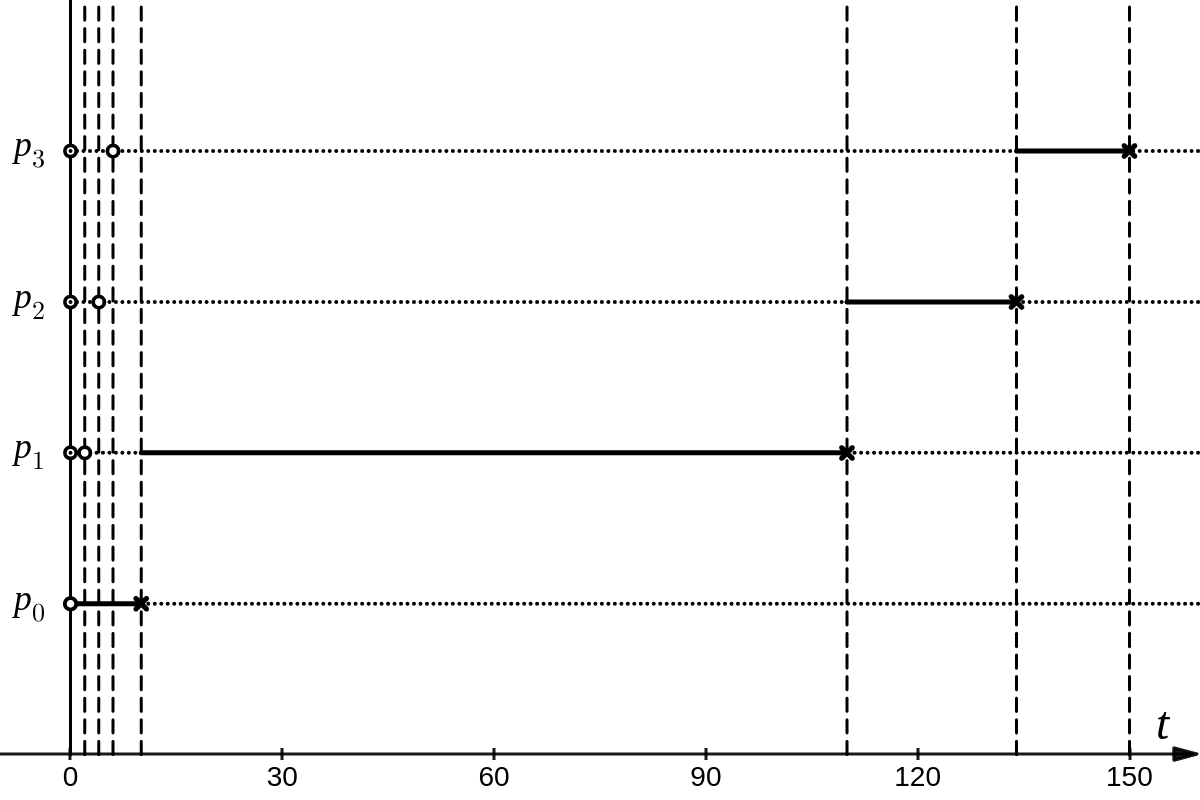
\includegraphics[scale=0.3]{../figures/fcfs_bad.png}
\end{center}

Questo risulta in un tempo medio di attesa di:
$$
\tilde{t}_a = \frac{{t_a}_0 + {t_a}_1 + {t_a}_2 + {t_a}_3}{4} = \frac{0 + 8 + 106 + 128}{4} = 60.5
$$

Vediamo come questo comportamento può cambiare radicalmente cambiando l'ordine di richiesta dei processi. Poniamo infatti di avere la sequenza:
\begin{table}[H]
	\center \rowcolors{2}{white}{black!10}
	\begin{tabular} { c || c | c }
		\bfseries Processo & \bfseries $\mathbf{T}$ richiesta & \bfseries $\mathbf{C}$ esecuzione \\
		\hline
		$p_0$ & 0 & 10 \\ 
		$p_1$ & 6 & 100 \\ 
		$p_2$ & 4 & 24 \\ 
		$p_3$ & 2 & 16 
	\end{tabular}
\end{table}
dove semplicemente si è invertito l'ordine degli ultimi 3 processi. 

\newpage

Sul grafico avremo:
\begin{center}
	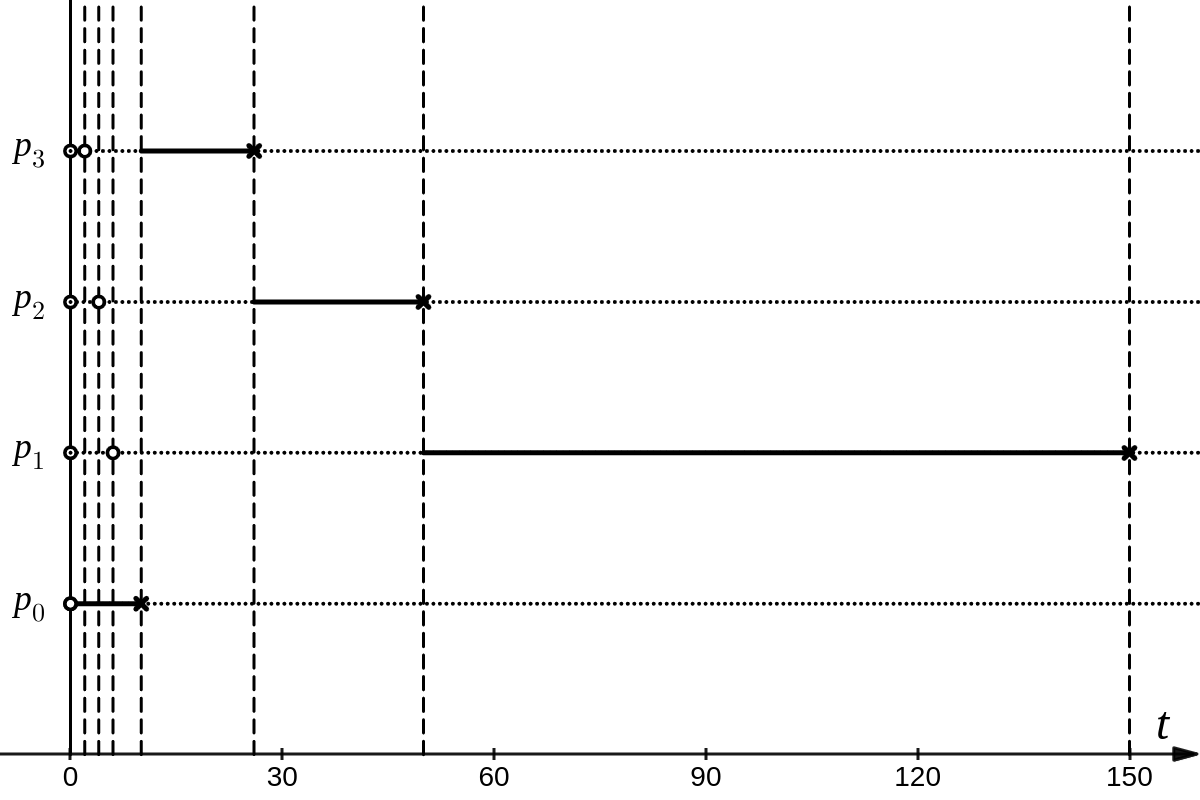
\includegraphics[scale=0.3]{../figures/fcfs_good.png}
\end{center}

Questo risulta in un tempo medio di attesa di:
$$
\tilde{t}_a = \frac{{t_a}_0 + {t_a}_1 + {t_a}_2 + {t_a}_3}{4} = \frac{0 + 44 + 22 + 8}{4} = 18.5
$$
Chiaramente molto meglio del caso precedente.

\par\smallskip

Abbiamo quindi che l'algoritmo è utile per sistemi batch, dove l'unica cosa che ci interessa è uso massimo della CPU (che ci assicura), ma largamente da evitare per sistemi interattivi, e sopratutto per sistemi real-time.
Questo è vouto all'aleatorietà legata al momento della richiesta dei processi, che rende impossibile rispondere celeremente o fare qualsiasi tipo di promessa sul tempo di turnaround.

\subsubsection{Algoritmo SJF}
L'algoritmo \textbf{SJF} (\textit{Shortest Job First}) implementa una \textbf{priorità statica}: si fa l'ipotesi di conoscere il \textbf{tempo di CPU} utilizzato da ogni processo, e assegnare priorità maggiori a processi con tempo di esecuzione minore. Di contro, non è preemptive, cioè una volta assegnata la CPU non può revocarla. Su come il S/O conosce il tempo di esecuzione non facciamo per adesso ipotesi. 

\par\smallskip

Simuliamo anche questo algoritmo, usando la stessa tabella del primo caso in 6.2.2:
\begin{table}[H]
	\center \rowcolors{2}{white}{black!10}
	\begin{tabular} { c || c | c }
		\bfseries Processo & \bfseries $\mathbf{T}$ richiesta & \bfseries $\mathbf{C}$ esecuzione \\
		\hline
		$p_0$ & 0 & 10 \\ 
		$p_1$ & 2 & 100 \\ 
		$p_2$ & 4 & 24 \\ 
		$p_3$ & 6 & 16 
	\end{tabular}
\end{table}

\newpage

Osserviamo che applicando l'algoritmo si ottiene il flusso di esecuzione:
\begin{center}
	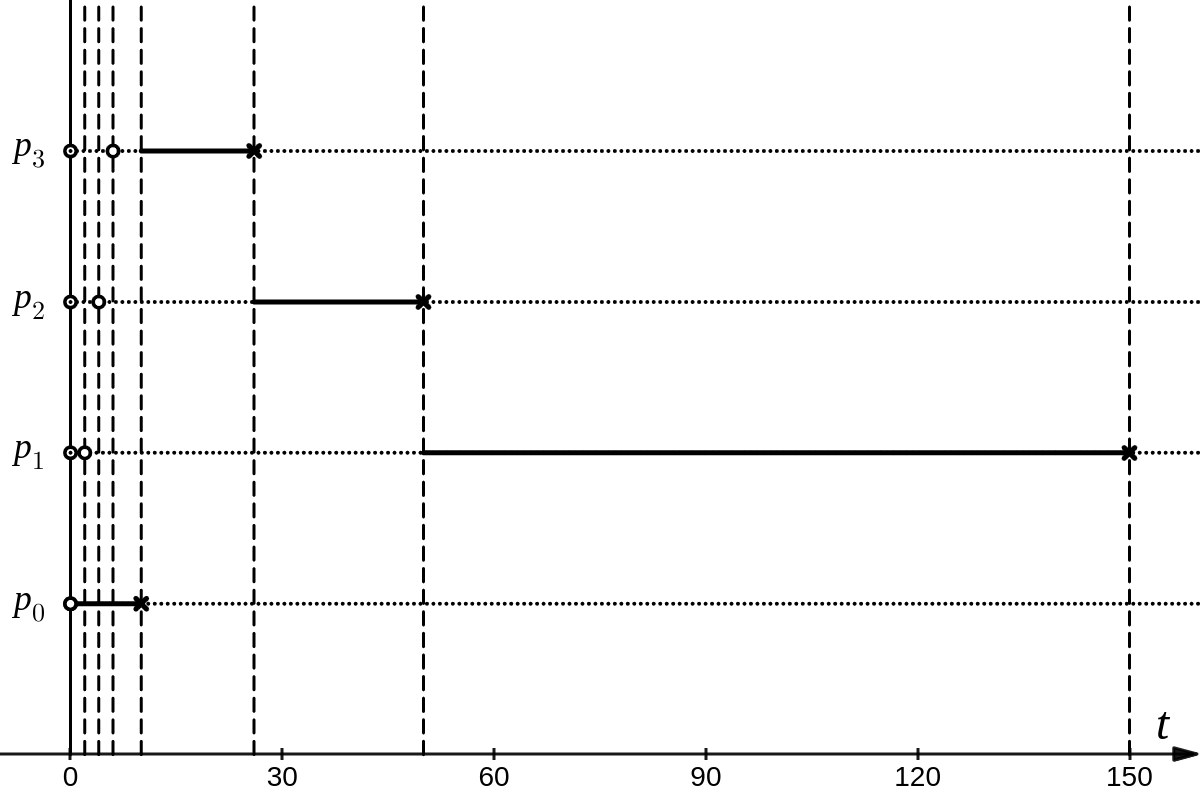
\includegraphics[scale=0.3]{../figures/sjf.png}
\end{center}
Cioè esattamente quello che avevamo visto come caso ottimo del FCFS (che ricordiamo aveva tempo medio $\tilde{T}_a = 18.5$), senza che i processi siano arrivati necessariamente nell'ordine ottimo.

\par\smallskip

Facciamo una nota sulla priorità statica: ad ogni chiamata dello scheduler questo può sapere solo i tempi di esecuzione dei processi attualmente in esecuzione, cioè si potrebbe mandare in esecuzione un processo con tempo di esecuzione maggiore quando ne entra in coda pronti ne entra uno con tempo minore. 
In questo caso, per la natura \textit{non preemptive} dell'algoritmo, bisogna lasciare che questo esegua prima di mettere il nuovo arrivato in esecuzione.

Adoperando questo algoritmo si minimizza (nel senso matematicamente ottimo) il tempo di attesa medio dei processi, in quanto si cerca di arrivare il prima possibile al processo sucessivo (svolgendo adesso il più veloce).
Uno svantaggio sarà chiaramente che i processi che dimostrano tempi di esecuzione lunghi verranno eseguiti sempre per ultimi.

\subsubsection{Algoritmo SRTF}
Abbiamo introdotto l'algoritmo \textbf{SRTF} (\textit{Shortest Remaining Time First}) come una versione \textit{preemptive} del SJF (in questo rimane comunque prioritario).

Visto che è preemptive, viene eseguito \textit{ogni volta} che cambiano le condizioni di scelta (non soltanto quando la CPU è libera, come nel caso dei non preemptive, ma ogni che un nuovo processo entra in esecuzione).
Può per questo motivo eseguire senza innescare cambi di contesto.

Dovremmo adattare la nostra ipotesi di conoscenza del tempo di CPU ad un'ipotesi di conoscenza del \textbf{tempo rimanente} per ogni processo: in questo caso se il processo appena entrato ha tempo rimanente minore di quello del processo attualmente in esecuzione, conviene sfruttare la preemption.
Di nuovo, per adesso non facciamo assunzioni su come ricaviamo tale euristica.

L'unica considerazione che ci conviene fare è che aggiornare le previsioni temporali ad ogni evento che cambia le condizioni di scelta chiede allo scheduler di fare più conti, e quindi aumenta leggermente l'overhead $O_v$.
Ampia letteratura dimostra che l'approccio è comunque conveniente. 

\par\smallskip

Simuliamo questo algoritmo con la tabella, modificata dalle precedenti mandando per primo in esecuzione il processo $p_1$, con tempo di esecuzione maggiore:
\begin{table}[H]
	\center \rowcolors{2}{white}{black!10}
	\begin{tabular} { c || c | c }
		\bfseries Processo & \bfseries $\mathbf{T}$ richiesta & \bfseries $\mathbf{C}$ esecuzione \\
		\hline
		$p_0$ & 2 & 10 \\ 
		$p_1$ & 0 & 100 \\ 
		$p_2$ & 4 & 24 \\ 
		$p_3$ & 6 & 16 
	\end{tabular}
\end{table}

Osserviamo che applicando l'algoritmo si ottiene il flusso di esecuzione:
\begin{center}
	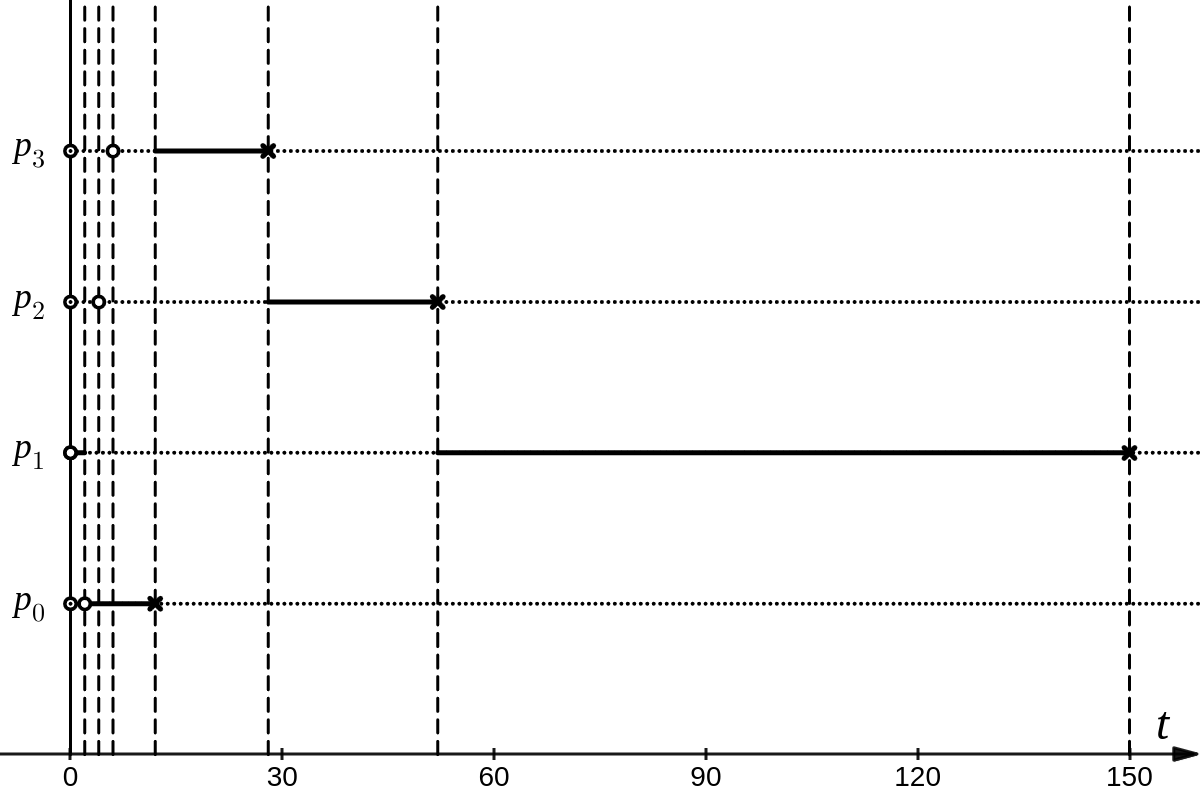
\includegraphics[scale=0.3]{../figures/srtf.png}
\end{center}

Questo risulta in un tempo medio di attesa di:
$$
\tilde{t}_a = \frac{{t_a}_0 + {t_a}_1 + {t_a}_2 + {t_a}_3}{4} = \frac{2 + 0 + 28 + 12}{4} = 10.5
$$
prima del primo burst.

Ciò che è importante in questo caso è che il processo $p_1$ viene sospeso con preemption per permettere l'esecuzione dei CPU burst di $p_0$, $p_2$ e $p_3$, molto più veloci. In questo modo il sistema risulta nel complesso molto più responsivo.

\par\smallskip

L'SRTF migliora la risposta in tempo reale del SJF, permettendo una riduzione sia dei tempi di turnaround che dei tempi di attesa medi in caso di richieste di esecuzione di processi non ottimali. 

Un problema del SRTF, come avevamo visto nel SJF, e la \textbf{process starvation}: in genere, negli algoritmi in base prioritaria, si rischia che i processi a priorità minore (in questo caso quelli con tempo rimanente maggiore) non vengano mai serviti e rimangano a lungo in coda pronti, rendendo il sistema meno responsivo.

Anche qui la letteratura ci rende noto che la priorità dei processi in SRTF è \textbf{monotona crescente}: man di mano che i processi eseguono, il loro tempo rimanente diminuisce e quindi la priorità aumenta. Questo effetto aiuta a ridurre la process starvation.

\subsubsection{Stima dei tempi in SJF e SRTF}
Chiariamo la questione di come si possono fare previsioni informate sul \textbf{tempo di esecuzione} (in \textit{SJF}) e il \textbf{tempo rimanente} (in \textit{SRTF}).

Un'approccio, preso ad esempio il caso del \textbf{tempo di esecuzione}, è quello di usare la tecnica della \textbf{esponenziale}.
Si fa una stima iniziale $s_i$ del tempo di burst $t_i$ esimo.
Preso un parametro $a$ con $0 < a < 1$, si aggiorna ad ogni terminazione del processo (quindi facendo delle \textit{osservazioni} per ogni esecuzione del processo) la stima come:
$$
s_{n + 1} = a t_n + (1 - a) s_n
$$

Presi $a \sim 0$ si ha che le stime deviano malvolentieri da quella iniziale, mentre con $a \sim 1$ si ha che le stime sono molto volubili rispetto alle osservazioni fatte. 

Modeli statistici più complessi possono dare previsioni più accurate, sempre tenendo conto del fatto che lo scheduler deve eseguire con overhead $O_v \sim 0$, o almeno il più piccolo possibile.

Una volta noto il \textit{tempo di esecuzione}, il \textbf{tempo rimanente} si può stimare considerando il tempo che il processo ha impiegato finora e sottraendolo dal tempo di esecuzione totale (se non rinunciando al tener conto se tale tempo è stato usato in CPU o I/O burst, purtroppo un'euristica è un'euristica).

\end{document}

\documentclass[a4paper,11pt]{article}
\usepackage[a4paper, margin=8em]{geometry}

% usa i pacchetti per la scrittura in italiano
\usepackage[french,italian]{babel}
\usepackage[T1]{fontenc}
\usepackage[utf8]{inputenc}
\frenchspacing 

% usa i pacchetti per la formattazione matematica
\usepackage{amsmath, amssymb, amsthm, amsfonts}

% usa altri pacchetti
\usepackage{gensymb}
\usepackage{hyperref}
\usepackage{standalone}

\usepackage{colortbl}

\usepackage{xstring}
\usepackage{karnaugh-map}

% imposta il titolo
\title{Appunti Sistemi Operativi}
\author{Luca Seggiani}
\date{2025}

% imposta lo stile
% usa helvetica
\usepackage[scaled]{helvet}
% usa palatino
\usepackage{palatino}
% usa un font monospazio guardabile
\usepackage{lmodern}

\renewcommand{\rmdefault}{ppl}
\renewcommand{\sfdefault}{phv}
\renewcommand{\ttdefault}{lmtt}

% circuiti
\usepackage{circuitikz}
\usetikzlibrary{babel}

% testo cerchiato
\newcommand*\circled[1]{\tikz[baseline=(char.base)]{
            \node[shape=circle,draw,inner sep=2pt] (char) {#1};}}

% disponi il titolo
\makeatletter
\renewcommand{\maketitle} {
	\begin{center} 
		\begin{minipage}[t]{.8\textwidth}
			\textsf{\huge\bfseries \@title} 
		\end{minipage}%
		\begin{minipage}[t]{.2\textwidth}
			\raggedleft \vspace{-1.65em}
			\textsf{\small \@author} \vfill
			\textsf{\small \@date}
		\end{minipage}
		\par
	\end{center}

	\thispagestyle{empty}
	\pagestyle{fancy}
}
\makeatother

% disponi teoremi
\usepackage{tcolorbox}
\newtcolorbox[auto counter, number within=section]{theorem}[2][]{%
	colback=blue!10, 
	colframe=blue!40!black, 
	sharp corners=northwest,
	fonttitle=\sffamily\bfseries, 
	title=Teorema~\thetcbcounter: #2, 
	#1
}

% disponi definizioni
\newtcolorbox[auto counter, number within=section]{definition}[2][]{%
	colback=red!10,
	colframe=red!40!black,
	sharp corners=northwest,
	fonttitle=\sffamily\bfseries,
	title=Definizione~\thetcbcounter: #2,
	#1
}

% disponi codice
\usepackage{listings}
\usepackage[table]{xcolor}

\definecolor{codegreen}{rgb}{0,0.6,0}
\definecolor{codegray}{rgb}{0.5,0.5,0.5}
\definecolor{codepurple}{rgb}{0.58,0,0.82}
\definecolor{backcolour}{rgb}{0.95,0.95,0.92}

\lstdefinestyle{codestyle}{
		backgroundcolor=\color{black!5}, 
		commentstyle=\color{codegreen},
		keywordstyle=\bfseries\color{magenta},
		numberstyle=\sffamily\tiny\color{black!60},
		stringstyle=\color{green!50!black},
		basicstyle=\ttfamily\footnotesize,
		breakatwhitespace=false,         
		breaklines=true,                 
		captionpos=b,                    
		keepspaces=true,                 
		numbers=left,                    
		numbersep=5pt,                  
		showspaces=false,                
		showstringspaces=false,
		showtabs=false,                  
		tabsize=2
}

\lstdefinestyle{shellstyle}{
		backgroundcolor=\color{black!5}, 
		basicstyle=\ttfamily\footnotesize\color{black}, 
		commentstyle=\color{black}, 
		keywordstyle=\color{black},
		numberstyle=\color{black!5},
		stringstyle=\color{black}, 
		showspaces=false,
		showstringspaces=false, 
		showtabs=false, 
		tabsize=2, 
		numbers=none, 
		breaklines=true
}


\lstdefinelanguage{assembler}{ 
  keywords={AAA, AAD, AAM, AAS, ADC, ADCB, ADCW, ADCL, ADD, ADDB, ADDW, ADDL, AND, ANDB, ANDW, ANDL,
        ARPL, BOUND, BSF, BSFL, BSFW, BSR, BSRL, BSRW, BSWAP, BT, BTC, BTCB, BTCW, BTCL, BTR, 
        BTRB, BTRW, BTRL, BTS, BTSB, BTSW, BTSL, CALL, CBW, CDQ, CLC, CLD, CLI, CLTS, CMC, CMP,
        CMPB, CMPW, CMPL, CMPS, CMPSB, CMPSD, CMPSW, CMPXCHG, CMPXCHGB, CMPXCHGW, CMPXCHGL,
        CMPXCHG8B, CPUID, CWDE, DAA, DAS, DEC, DECB, DECW, DECL, DIV, DIVB, DIVW, DIVL, ENTER,
        HLT, IDIV, IDIVB, IDIVW, IDIVL, IMUL, IMULB, IMULW, IMULL, IN, INB, INW, INL, INC, INCB,
        INCW, INCL, INS, INSB, INSD, INSW, INT, INT3, INTO, INVD, INVLPG, IRET, IRETD, JA, JAE,
        JB, JBE, JC, JCXZ, JE, JECXZ, JG, JGE, JL, JLE, JMP, JNA, JNAE, JNB, JNBE, JNC, JNE, JNG,
        JNGE, JNL, JNLE, JNO, JNP, JNS, JNZ, JO, JP, JPE, JPO, JS, JZ, LAHF, LAR, LCALL, LDS,
        LEA, LEAVE, LES, LFS, LGDT, LGS, LIDT, LMSW, LOCK, LODSB, LODSD, LODSW, LOOP, LOOPE,
        LOOPNE, LSL, LSS, LTR, MOV, MOVB, MOVW, MOVL, MOVSB, MOVSD, MOVSW, MOVSX, MOVSXB,
        MOVSXW, MOVSXL, MOVZX, MOVZXB, MOVZXW, MOVZXL, MUL, MULB, MULW, MULL, NEG, NEGB, NEGW,
        NEGL, NOP, NOT, NOTB, NOTW, NOTL, OR, ORB, ORW, ORL, OUT, OUTB, OUTW, OUTL, OUTSB, OUTSD,
        OUTSW, POP, POPL, POPW, POPB, POPA, POPAD, POPF, POPFD, PUSH, PUSHL, PUSHW, PUSHB, PUSHA, 
				PUSHAD, PUSHF, PUSHFD, RCL, RCLB, RCLW, MOVSL, MOVSB, MOVSW, STOSL, STOSB, STOSW, LODSB, LODSW,
				LODSL, INSB, INSW, INSL, OUTSB, OUTSL, OUTSW
        RCLL, RCR, RCRB, RCRW, RCRL, RDMSR, RDPMC, RDTSC, REP, REPE, REPNE, RET, ROL, ROLB, ROLW,
        ROLL, ROR, RORB, RORW, RORL, SAHF, SAL, SALB, SALW, SALL, SAR, SARB, SARW, SARL, SBB,
        SBBB, SBBW, SBBL, SCASB, SCASD, SCASW, SETA, SETAE, SETB, SETBE, SETC, SETE, SETG, SETGE,
        SETL, SETLE, SETNA, SETNAE, SETNB, SETNBE, SETNC, SETNE, SETNG, SETNGE, SETNL, SETNLE,
        SETNO, SETNP, SETNS, SETNZ, SETO, SETP, SETPE, SETPO, SETS, SETZ, SGDT, SHL, SHLB, SHLW,
        SHLL, SHLD, SHR, SHRB, SHRW, SHRL, SHRD, SIDT, SLDT, SMSW, STC, STD, STI, STOSB, STOSD,
        STOSW, STR, SUB, SUBB, SUBW, SUBL, TEST, TESTB, TESTW, TESTL, VERR, VERW, WAIT, WBINVD,
        XADD, XADDB, XADDW, XADDL, XCHG, XCHGB, XCHGW, XCHGL, XLAT, XLATB, XOR, XORB, XORW, XORL},
  keywordstyle=\color{blue}\bfseries,
  ndkeywordstyle=\color{darkgray}\bfseries,
  identifierstyle=\color{black},
  sensitive=false,
  comment=[l]{\#},
  morecomment=[s]{/*}{*/},
  commentstyle=\color{purple}\ttfamily,
  stringstyle=\color{red}\ttfamily,
  morestring=[b]',
  morestring=[b]"
}

\lstset{language=assembler, style=codestyle}

% disponi sezioni
\usepackage{titlesec}

\titleformat{\section}
	{\sffamily\Large\bfseries} 
	{\thesection}{1em}{} 
\titleformat{\subsection}
	{\sffamily\large\bfseries}   
	{\thesubsection}{1em}{} 
\titleformat{\subsubsection}
	{\sffamily\normalsize\bfseries} 
	{\thesubsubsection}{1em}{}

% tikz
\usepackage{tikz}

% float
\usepackage{float}

% grafici
\usepackage{pgfplots}
\pgfplotsset{width=10cm,compat=1.9}

% disponi alberi
\usepackage{forest}

\forestset{
	rectstyle/.style={
		for tree={rectangle,draw,font=\large\sffamily}
	},
	roundstyle/.style={
		for tree={circle,draw,font=\large}
	}
}

% disponi algoritmi
\usepackage{algorithm}
\usepackage{algorithmic}
\makeatletter
\renewcommand{\ALG@name}{Algoritmo}
\makeatother

% disponi numeri di pagina
\usepackage{fancyhdr}
\fancyhf{} 
\fancyfoot[L]{\sffamily{\thepage}}

\makeatletter
\fancyhead[L]{\raisebox{1ex}[0pt][0pt]{\sffamily{\@title \ \@date}}} 
\fancyhead[R]{\raisebox{1ex}[0pt][0pt]{\sffamily{\@author}}}
\makeatother

\begin{document}
% sezione (data)
\section{Lezione del 08-10-25}

% stili pagina
\thispagestyle{empty}
\pagestyle{fancy}

% testo
Continuiamo la discussione degli algoritmi di scheduling.

\subsubsection{Algoritmo RR}
L'algoritmo \textbf{RR} (\textit{Round Robin}) è preemptive e non prioritario, e si basa su un meccanismo molto semplice: ad ogni processo viene dato un quanto temporale prefissato, e via preemption si passa al processo successivo quando tale quanto viene esaurito.

Questo lo rende molto efficiente: l'overhead $O_v$ è minimo, quasi al pari di FCFS (leggermente più alto in quanto i cambi di contesto sono più frequenti, uno ogni quanto temporale). 
\par\smallskip

Simuliamo questo algoritmo usando la sequenza di processi richiesti già vista in 6.2.2, e imponendo un quanto temporale di $\Delta T = 20$. La tabella dei tempi di richiesta e esecuzione dei processi sarà:
\begin{table}[H]
	\center \rowcolors{2}{white}{black!10}
	\begin{tabular} { c || c | c }
		\bfseries Processo & \bfseries $\mathbf{T}$ richiesta & \bfseries $\mathbf{C}$ esecuzione \\
		\hline
		$p_0$ & 0 & 10 \\ 
		$p_1$ & 2 & 100 \\ 
		$p_2$ & 4 & 24 \\ 
		$p_3$ & 6 & 16 
	\end{tabular}
\end{table}

\newpage

In questo caso la \textit{timeline} avrà un aspetto del genere:
\begin{center}
	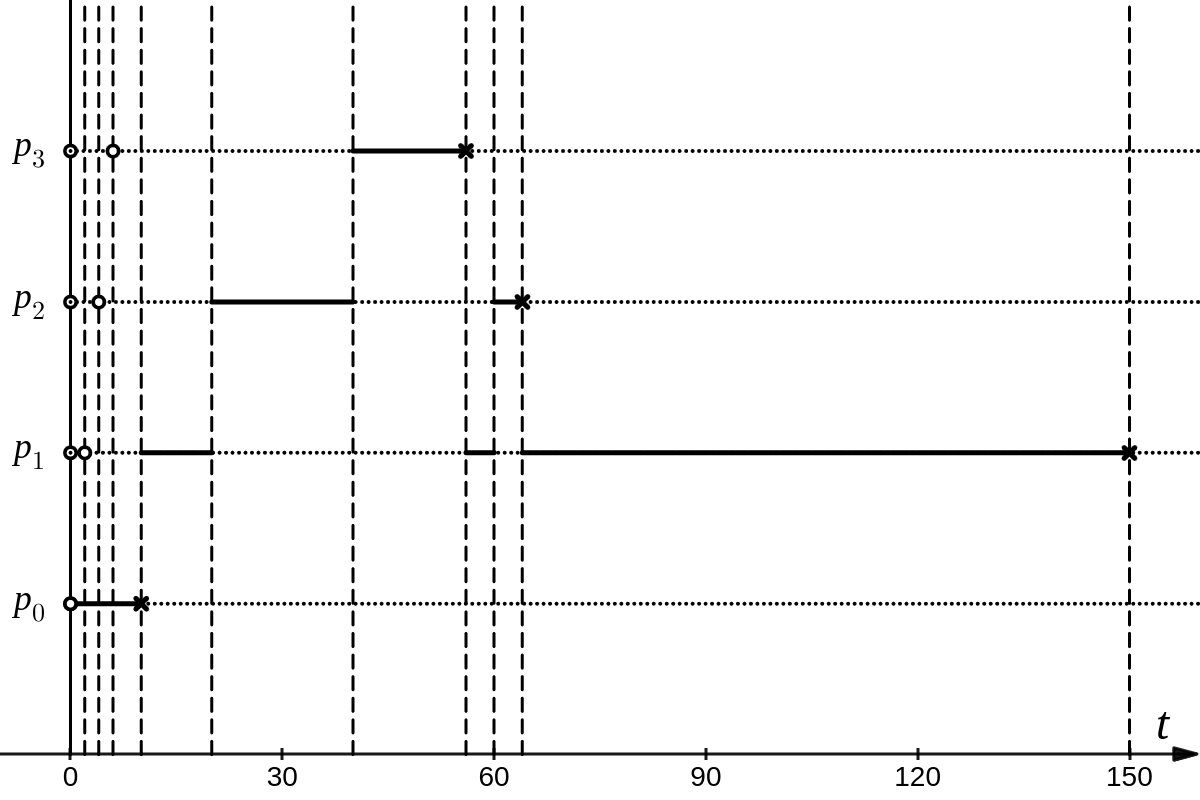
\includegraphics[scale=0.3]{../figures/rr.png}
\end{center}

Vediamo che il tempo medio, calcolato come:
$$
\tilde{t}_a = \frac{{t_a}_0 + {t_a}_1 + {t_a}_2 + {t_a}_3}{4} = \frac{0 + 10 + 20 + 40}{4} = 17.5
$$
sarà più o meno nella norma rispetto a SJR o STRF.

La cosa importante è, come lo era stato per STRF, la \textit{responsività} che l'algoritmo riesce a realizzare: un processo non resta mai in coda pronti per un tempo maggiore al quanto temporale moltiplicato per i processi in esecuzione meno 1.

\par\smallskip

Dal punto di vista implementativo, organizzaremo i quanti temporali sfruttando una componente hardware detta \textbf{timer}: questo è considerato a tutti gli effetti una periferiche, ed invia (dopo un'opportuna configurazione) interruzioni esterne periodiche.
Ogni volta che il processore riceve tale interruzione, mette in esecuzione lo scheduler, che provvede a cambiare il contesto al prossimo processo.
Chiaramente, lo scheduler può comunque essere messo in esecuzione da eventi comuni come la terminazione di processi.

Per realizzare l'esecuzione ciclica si usa una semplice coda pronti dove lo scheduler estreae sempre dalla testa e inserisce sempre in fondo alla coda.

Come abbiamo visto dall'esempio, l'RR rende molto semplice stimare il tempo di attesa: se ci sono $N$ processi in esecuzione, $N - 1$ saranno in coda pronti in qualsiasi momento, quindi un dato processo aspetterà:
$$
T_a = (N - 1)q
$$
dove $q$ è il quanto di tempo.

Chiaramente il $T_a$ diventa troppo grande se ci sono troppi processi.

\subsection{Code multilivello}
Abbiamo quindi discusso i 4 algoritmi di scheduling fondamentali che avevamo introdotto in 6.2.
Ognuno di questi ha pro e contro distinti, ed è più adeguato in una o un altra situazione.

Per questo motivo nei sistemi operativi moderni si preferisce implementare lo scheduling attraverso \textbf{più algoritmi} di scheduling, che gestiscono ognuno la situazione che più conviene.

Un modo elegante di realizzare ciò è mantenere \textbf{più code}, una per ogni algoritmo di scheduling. Sistemi di questo tipo vengono detti \textbf{multilevel queue} o \textit{code multilivello}.

\subsubsection{Code di feedback}
Una variante interessante delle code multilivello è dato dalle \textit{code di feedback}.
Queste nascono per gestire più gerarchie di processi dai requisiti di esecuzione diversi (I/O bound, più interattivi, e CPU bound, più lenti).

In questo caso si prevede una struttura di code, ad esempio come la seguente:
\begin{enumerate}
	\item Coda RR \textit{veloce}, con quanto $\Delta T = 10$;
	\item Coda RR \textit{più lenta}, con quanto $\Delta T = 20$;
	\item Coda FCFS, la più \textit{lenta}.
\end{enumerate}
Le code vengono ordinate per priorità decrescente.

Un processo richiesto viene messo nella coda RR più veloce: se al momento della prima revoca CPU non è riuscito a terminare il suo primo CPU burst, viene spostato nella coda RR più lenta.
La procedura si ripete finché il processo non è giudicato come \textit{non interattivo} e spostato nella coda FCFS.

In questo modo si riescono a sviluppare sistemi che si \textit{"adattano"} in qualche modo a diversi tipi di processi, scegliendo per ognuno la coda (e quindi la politica di schedulazione) più adatta.

\par\smallskip

Facciamo qualche altra considerazione: poniamo che ci sia un processo molto interattivo (magari il processo che si occupa di disegnare l'ambiente grafico) nella prima coda, e un processo CPU bound molto lento (magari un software di calcolo scientifico) in coda FCFS.

Avremo che il processo interattivo farà molti I/O burst (scrittura a video, lettura dati da mouse e tastiera, ecc...) e probabilmente i suoi CPU burst finiranno prima del quanto temporale offerto dalla coda RR.
Sarà in questi istanti che il processo lento potrà entrare in esecuzione nella coda FCFS.

\par\smallskip

L'approccio non è ideale in quanto presenta alcuni difetti:
\begin{itemize}
	\item 
Potrebbero verificarsi casi dove il processo in coda FCFS non riesce ad eseguire di fronte a una grande massa di processi veloci che arrivano in coda RR (\textit{starvation}): per questo motivo gli S/O moderni implementano altri meccanismi, come l'\textit{aging};
	\item
Un'altra problematica è data dal fatto che l'ultima coda è non preemptive: quando un processo dal lungo CPU Burst entra in coda FCFS vi resta finche non ha finito di eseguire, bloccando il resto del sistema. 

Possiamo risolvere questo problema rendendo l'FCFS vagamente \textit{preemptive}: visto che ci sono altre due code prima di essa, possiamo cogliere l'occasione del lancio di un nuovo processo per rimettere in esecuzione lo scheduler. Questo meccanismo non è propriamente necessaria per le prime 2 code in quanto il quanto di tempo è limitato (e quindi prima o poi il nuovo processo viene servito), mentre è fondamentale per la coda FCFS che potrebbe bloccare anche per diverso tempo.
\end{itemize}

Un ultima considerazione che vogliamo fare è se \textit{conviene} riportare i processi dalle code di livello inferiore (più lente) nelle code di livello superiore (più veloci) quando queste si sgombrano: in generale, abbiamo che la letteratura non lo trova particolarmente vantaggioso.
Questo perché un processo che è finito in una coda meno interattiva è probabilmente \textit{meno interattivo}, per cui può godere di CPU burst più lunghi e deve restare nella coda dove si trova.

In caso di \textit{aging}, di contro, questo processo è necessario e più che naturale: spostiamo i processi che sono da molto tempo in code inferiori verso le code superiori per forzarne l'esecuzione.

\end{document}

\documentclass[a4paper,11pt]{article}
\usepackage[a4paper, margin=8em]{geometry}

% usa i pacchetti per la scrittura in italiano
\usepackage[french,italian]{babel}
\usepackage[T1]{fontenc}
\usepackage[utf8]{inputenc}
\frenchspacing 

% usa i pacchetti per la formattazione matematica
\usepackage{amsmath, amssymb, amsthm, amsfonts}

% usa altri pacchetti
\usepackage{gensymb}
\usepackage{hyperref}
\usepackage{standalone}

\usepackage{colortbl}

\usepackage{xstring}
\usepackage{karnaugh-map}

% imposta il titolo
\title{Appunti Sistemi Operativi}
\author{Luca Seggiani}
\date{2025}

% imposta lo stile
% usa helvetica
\usepackage[scaled]{helvet}
% usa palatino
\usepackage{palatino}
% usa un font monospazio guardabile
\usepackage{lmodern}

\renewcommand{\rmdefault}{ppl}
\renewcommand{\sfdefault}{phv}
\renewcommand{\ttdefault}{lmtt}

% circuiti
\usepackage{circuitikz}
\usetikzlibrary{babel}

% testo cerchiato
\newcommand*\circled[1]{\tikz[baseline=(char.base)]{
            \node[shape=circle,draw,inner sep=2pt] (char) {#1};}}

% disponi il titolo
\makeatletter
\renewcommand{\maketitle} {
	\begin{center} 
		\begin{minipage}[t]{.8\textwidth}
			\textsf{\huge\bfseries \@title} 
		\end{minipage}%
		\begin{minipage}[t]{.2\textwidth}
			\raggedleft \vspace{-1.65em}
			\textsf{\small \@author} \vfill
			\textsf{\small \@date}
		\end{minipage}
		\par
	\end{center}

	\thispagestyle{empty}
	\pagestyle{fancy}
}
\makeatother

% disponi teoremi
\usepackage{tcolorbox}
\newtcolorbox[auto counter, number within=section]{theorem}[2][]{%
	colback=blue!10, 
	colframe=blue!40!black, 
	sharp corners=northwest,
	fonttitle=\sffamily\bfseries, 
	title=Teorema~\thetcbcounter: #2, 
	#1
}

% disponi definizioni
\newtcolorbox[auto counter, number within=section]{definition}[2][]{%
	colback=red!10,
	colframe=red!40!black,
	sharp corners=northwest,
	fonttitle=\sffamily\bfseries,
	title=Definizione~\thetcbcounter: #2,
	#1
}

% disponi codice
\usepackage{listings}
\usepackage[table]{xcolor}

\definecolor{codegreen}{rgb}{0,0.6,0}
\definecolor{codegray}{rgb}{0.5,0.5,0.5}
\definecolor{codepurple}{rgb}{0.58,0,0.82}
\definecolor{backcolour}{rgb}{0.95,0.95,0.92}

\lstdefinestyle{codestyle}{
		backgroundcolor=\color{black!5}, 
		commentstyle=\color{codegreen},
		keywordstyle=\bfseries\color{magenta},
		numberstyle=\sffamily\tiny\color{black!60},
		stringstyle=\color{green!50!black},
		basicstyle=\ttfamily\footnotesize,
		breakatwhitespace=false,         
		breaklines=true,                 
		captionpos=b,                    
		keepspaces=true,                 
		numbers=left,                    
		numbersep=5pt,                  
		showspaces=false,                
		showstringspaces=false,
		showtabs=false,                  
		tabsize=2
}

\lstdefinestyle{shellstyle}{
		backgroundcolor=\color{black!5}, 
		basicstyle=\ttfamily\footnotesize\color{black}, 
		commentstyle=\color{black}, 
		keywordstyle=\color{black},
		numberstyle=\color{black!5},
		stringstyle=\color{black}, 
		showspaces=false,
		showstringspaces=false, 
		showtabs=false, 
		tabsize=2, 
		numbers=none, 
		breaklines=true
}


\lstdefinelanguage{assembler}{ 
  keywords={AAA, AAD, AAM, AAS, ADC, ADCB, ADCW, ADCL, ADD, ADDB, ADDW, ADDL, AND, ANDB, ANDW, ANDL,
        ARPL, BOUND, BSF, BSFL, BSFW, BSR, BSRL, BSRW, BSWAP, BT, BTC, BTCB, BTCW, BTCL, BTR, 
        BTRB, BTRW, BTRL, BTS, BTSB, BTSW, BTSL, CALL, CBW, CDQ, CLC, CLD, CLI, CLTS, CMC, CMP,
        CMPB, CMPW, CMPL, CMPS, CMPSB, CMPSD, CMPSW, CMPXCHG, CMPXCHGB, CMPXCHGW, CMPXCHGL,
        CMPXCHG8B, CPUID, CWDE, DAA, DAS, DEC, DECB, DECW, DECL, DIV, DIVB, DIVW, DIVL, ENTER,
        HLT, IDIV, IDIVB, IDIVW, IDIVL, IMUL, IMULB, IMULW, IMULL, IN, INB, INW, INL, INC, INCB,
        INCW, INCL, INS, INSB, INSD, INSW, INT, INT3, INTO, INVD, INVLPG, IRET, IRETD, JA, JAE,
        JB, JBE, JC, JCXZ, JE, JECXZ, JG, JGE, JL, JLE, JMP, JNA, JNAE, JNB, JNBE, JNC, JNE, JNG,
        JNGE, JNL, JNLE, JNO, JNP, JNS, JNZ, JO, JP, JPE, JPO, JS, JZ, LAHF, LAR, LCALL, LDS,
        LEA, LEAVE, LES, LFS, LGDT, LGS, LIDT, LMSW, LOCK, LODSB, LODSD, LODSW, LOOP, LOOPE,
        LOOPNE, LSL, LSS, LTR, MOV, MOVB, MOVW, MOVL, MOVSB, MOVSD, MOVSW, MOVSX, MOVSXB,
        MOVSXW, MOVSXL, MOVZX, MOVZXB, MOVZXW, MOVZXL, MUL, MULB, MULW, MULL, NEG, NEGB, NEGW,
        NEGL, NOP, NOT, NOTB, NOTW, NOTL, OR, ORB, ORW, ORL, OUT, OUTB, OUTW, OUTL, OUTSB, OUTSD,
        OUTSW, POP, POPL, POPW, POPB, POPA, POPAD, POPF, POPFD, PUSH, PUSHL, PUSHW, PUSHB, PUSHA, 
				PUSHAD, PUSHF, PUSHFD, RCL, RCLB, RCLW, MOVSL, MOVSB, MOVSW, STOSL, STOSB, STOSW, LODSB, LODSW,
				LODSL, INSB, INSW, INSL, OUTSB, OUTSL, OUTSW
        RCLL, RCR, RCRB, RCRW, RCRL, RDMSR, RDPMC, RDTSC, REP, REPE, REPNE, RET, ROL, ROLB, ROLW,
        ROLL, ROR, RORB, RORW, RORL, SAHF, SAL, SALB, SALW, SALL, SAR, SARB, SARW, SARL, SBB,
        SBBB, SBBW, SBBL, SCASB, SCASD, SCASW, SETA, SETAE, SETB, SETBE, SETC, SETE, SETG, SETGE,
        SETL, SETLE, SETNA, SETNAE, SETNB, SETNBE, SETNC, SETNE, SETNG, SETNGE, SETNL, SETNLE,
        SETNO, SETNP, SETNS, SETNZ, SETO, SETP, SETPE, SETPO, SETS, SETZ, SGDT, SHL, SHLB, SHLW,
        SHLL, SHLD, SHR, SHRB, SHRW, SHRL, SHRD, SIDT, SLDT, SMSW, STC, STD, STI, STOSB, STOSD,
        STOSW, STR, SUB, SUBB, SUBW, SUBL, TEST, TESTB, TESTW, TESTL, VERR, VERW, WAIT, WBINVD,
        XADD, XADDB, XADDW, XADDL, XCHG, XCHGB, XCHGW, XCHGL, XLAT, XLATB, XOR, XORB, XORW, XORL},
  keywordstyle=\color{blue}\bfseries,
  ndkeywordstyle=\color{darkgray}\bfseries,
  identifierstyle=\color{black},
  sensitive=false,
  comment=[l]{\#},
  morecomment=[s]{/*}{*/},
  commentstyle=\color{purple}\ttfamily,
  stringstyle=\color{red}\ttfamily,
  morestring=[b]',
  morestring=[b]"
}

\lstset{language=assembler, style=codestyle}

% disponi sezioni
\usepackage{titlesec}

\titleformat{\section}
	{\sffamily\Large\bfseries} 
	{\thesection}{1em}{} 
\titleformat{\subsection}
	{\sffamily\large\bfseries}   
	{\thesubsection}{1em}{} 
\titleformat{\subsubsection}
	{\sffamily\normalsize\bfseries} 
	{\thesubsubsection}{1em}{}

% tikz
\usepackage{tikz}

% float
\usepackage{float}

% grafici
\usepackage{pgfplots}
\pgfplotsset{width=10cm,compat=1.9}

% disponi alberi
\usepackage{forest}

\forestset{
	rectstyle/.style={
		for tree={rectangle,draw,font=\large\sffamily}
	},
	roundstyle/.style={
		for tree={circle,draw,font=\large}
	}
}

% disponi algoritmi
\usepackage{algorithm}
\usepackage{algorithmic}
\makeatletter
\renewcommand{\ALG@name}{Algoritmo}
\makeatother

% disponi numeri di pagina
\usepackage{fancyhdr}
\fancyhf{} 
\fancyfoot[L]{\sffamily{\thepage}}

\makeatletter
\fancyhead[L]{\raisebox{1ex}[0pt][0pt]{\sffamily{\@title \ \@date}}} 
\fancyhead[R]{\raisebox{1ex}[0pt][0pt]{\sffamily{\@author}}}
\makeatother

\begin{document}
% sezione (data)
\section{Lezione del 14-10-25}

% stili pagina
\thispagestyle{empty}
\pagestyle{fancy}

% testo
\subsection{Schedulazione real-time}
Veniamo quindi a come implementare la schedulazione nei sistemi in \textbf{tempo reale}.
Avevamo detto che questi erano sistemi principalmente di tipo \textit{embedded}, cioè incorporati, non general-purpose ma \textit{special-purpose} atti a governare sistemi esterni (sistemi di controllo per veicoli, macchinari industriali, ecc...).

\subsubsection{Esecuzione ciclica}
Abbiamo che la caratteristica principale di sistemi di questo tipo è il tipo di periferiche con cui interagiscono: invece di periferiche multiple e variabili (come nei sistemi general-purpose), avremo un insieme fisso di dispositivi di ingresso (detti \textit{sensori}) e di uscita (detti \textit{attuatori}).

Questo porta ad un paradigma di esecuzione fortemente periodico: si campiona il sistema esterno attraverso i sensori, compie una qualche elaborazione, e aggiornano gli attuatori per rispondere a quanto rilevato.

Ciò significa che i processi messi in esecuzione devono rispettare il periodo dell'esecuzione ciclica, e produrre il loro risultato entro date \textit{scadenze} date dal periodo corrente e il numero di altri processi in esecuzione.
Occorre allora avere un controllo preciso e granulare sul tempo che impiegano a terminare. 

\subsubsection{Deadline}
In questo caso prevederemo, dopo l'istante di richiesta $r$ di un processo, una certa deadline $d$, calcolata come:
$$
d = r + \Delta d
$$
dove $\Delta d$ è il tempo massimo di esecuzione del processo.
\begin{itemize}
	\item In un sistema \textit{soft real-time} si cerca di fare il possibile per assicurare che il processo termini prima di $d$;
	\item In un sistema \textit{hard real-time} la terminazione del processo prima di $d$ è prerogativa dell'integrità dell'intero sistema.
\end{itemize}

In particolare, riguardo al paradigma di esecuzione ciclica accennato nello scorso paragrafo, avremo che per un processo che deve eseguire ciclicamente con periodo $\Delta t$, per ogni istante di richiesta $r_i$ l'istante di richista successivo sarà calcolato come:
$$
r_{i + 1} = r_i + \Delta t
$$
In questo caso sarà fondamentale rispettare la diseguaglianza:
$$
d_i < r_{i + 1} \ \Leftrightarrow \ \Delta d_i < \Delta t
$$
data $d_i$ come deadline dopo la richiesta $r_i$.

Estendo il concetto a sistemi multiprogrammati, avremo che dati $n$ processi il periodo $T$ di aggiornamento simultaneo di ogni processo in esecuzione sarà:
$$
T = \text{MCM}\left(\Delta t_i\right)
$$
con $t_i$ i periodi di ogni processo: semplicemente si prende il minimo comune multiplo.

\par\smallskip

Ritornando all'idea dei CPU burst, se il processo si svolge in più CPU burst $C_1$, $C_2$, ecc... dovrà quindi essere che:
$$
T_e = \sum C_i < \Delta d_i
$$
cioè che almeno il tempo di esecuzione del processo sia minore del tempo massimo di esecuzione per rispettare la deadline corrente.

\subsubsection{Algoritmo RM}
Iniziamo quindi a vedere alcuni algoritmi di scheduling per sistemi realtime.
Il primo che vediamo è l'\textbf{RM} (\textit{Rate Monotonic}).
Questo consiste semplicemente ad assegnare una priorità statica \textit{monotonica crescente} ai processi in base al \textit{rate}, cioè la frequenza, del loro ciclo di esecuzione.
Questo equivale ad assegnare una proprietà inversamente proporzionale al periodo $t$ del processo:
$$
p \propto \frac{1}{t} = f
$$

Visto che la proprietà è statica, chiaramente l'algoritmo è non preemptive.

\par\smallskip

Facciamo quindi l'esempio dell'esecuzione dell'algoritmo, ipotizzando due processi $p_a$ e $p_b$:
\begin{table}[H]
	\center \rowcolors{2}{white}{black!10}
	\begin{tabular} { c || c | c }
		\bfseries Processo & \bfseries $\Delta \mathbf{t}$ periodo & \bfseries $\mathbf{\Delta T}$ esecuzione \\
		\hline
		$p_a$ & 2 & 1 \\ 
		$p_b$ & 5 & 1
	\end{tabular}
\end{table}

Da questo è fra l'altro immediato che, con $\Delta t_a = 2$ e $\Delta t_b = 5$, il periodo complessivo di sistema $T$ è:
$$
T = \text{MCM}(\Delta t_a, \Delta t_b) = \text{MCM}(2, 5) = 10
$$

Vedremo come questo periodo determina anche il periodo dell'attività dello scheduler.

\newpage

Simulando l'esecuzione si ha, colorando in rosso le deadline di $p_a$ e in blu quelle di $p_b$:
\begin{center}
	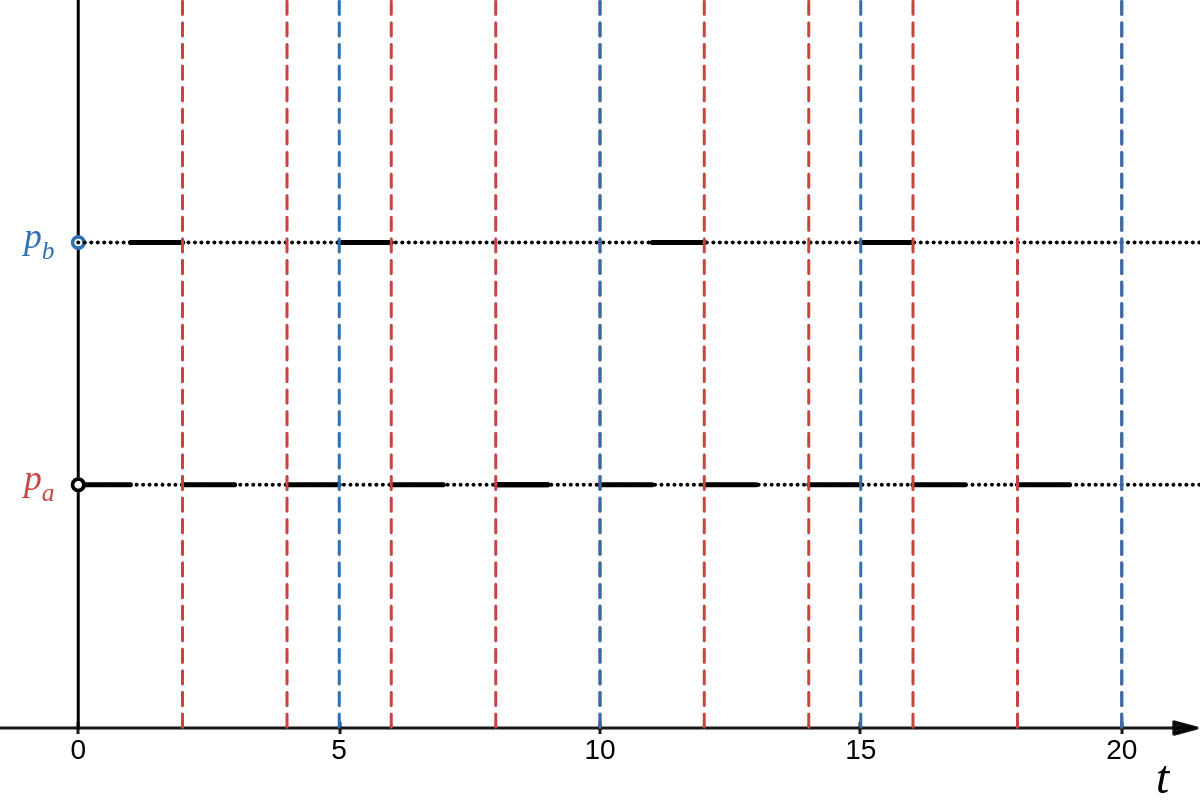
\includegraphics[scale=0.3]{../figures/rm.png}
\end{center}

Vediamo quindi come riusciamo a rispettare tutte le deadline.
Un problema è che, ad esempio all'istante 10, si sono fatti 3 cicli da un unità temporale a vuoto, cioè l'efficienza $E$ è:
$$
E = \frac{10 - 3}{10} = 70 \%
$$

Questo non è immediatamente sbagliato: significa solo che il sistema ha abbastanza risorse da soddisfare ampiamente le richieste in arrivo.
Potrebbe diventare un problema quando vogliamo \textit{"stringere"} le temporizzazioni in modo da far fronte ad un maggior numero di processi, o processi con CPU burst più consistenti.

\end{document}

\documentclass[a4paper,11pt]{article}
\usepackage[a4paper, margin=8em]{geometry}

% usa i pacchetti per la scrittura in italiano
\usepackage[french,italian]{babel}
\usepackage[T1]{fontenc}
\usepackage[utf8]{inputenc}
\frenchspacing 

% usa i pacchetti per la formattazione matematica
\usepackage{amsmath, amssymb, amsthm, amsfonts}

% usa altri pacchetti
\usepackage{gensymb}
\usepackage{hyperref}
\usepackage{standalone}

\usepackage{colortbl}

\usepackage{xstring}
\usepackage{karnaugh-map}

% imposta il titolo
\title{Appunti Sistemi Operativi}
\author{Luca Seggiani}
\date{2025}

% imposta lo stile
% usa helvetica
\usepackage[scaled]{helvet}
% usa palatino
\usepackage{palatino}
% usa un font monospazio guardabile
\usepackage{lmodern}

\renewcommand{\rmdefault}{ppl}
\renewcommand{\sfdefault}{phv}
\renewcommand{\ttdefault}{lmtt}

% circuiti
\usepackage{circuitikz}
\usetikzlibrary{babel}

% testo cerchiato
\newcommand*\circled[1]{\tikz[baseline=(char.base)]{
            \node[shape=circle,draw,inner sep=2pt] (char) {#1};}}

% disponi il titolo
\makeatletter
\renewcommand{\maketitle} {
	\begin{center} 
		\begin{minipage}[t]{.8\textwidth}
			\textsf{\huge\bfseries \@title} 
		\end{minipage}%
		\begin{minipage}[t]{.2\textwidth}
			\raggedleft \vspace{-1.65em}
			\textsf{\small \@author} \vfill
			\textsf{\small \@date}
		\end{minipage}
		\par
	\end{center}

	\thispagestyle{empty}
	\pagestyle{fancy}
}
\makeatother

% disponi teoremi
\usepackage{tcolorbox}
\newtcolorbox[auto counter, number within=section]{theorem}[2][]{%
	colback=blue!10, 
	colframe=blue!40!black, 
	sharp corners=northwest,
	fonttitle=\sffamily\bfseries, 
	title=Teorema~\thetcbcounter: #2, 
	#1
}

% disponi definizioni
\newtcolorbox[auto counter, number within=section]{definition}[2][]{%
	colback=red!10,
	colframe=red!40!black,
	sharp corners=northwest,
	fonttitle=\sffamily\bfseries,
	title=Definizione~\thetcbcounter: #2,
	#1
}

% disponi codice
\usepackage{listings}
\usepackage[table]{xcolor}

\definecolor{codegreen}{rgb}{0,0.6,0}
\definecolor{codegray}{rgb}{0.5,0.5,0.5}
\definecolor{codepurple}{rgb}{0.58,0,0.82}
\definecolor{backcolour}{rgb}{0.95,0.95,0.92}

\lstdefinestyle{codestyle}{
		backgroundcolor=\color{black!5}, 
		commentstyle=\color{codegreen},
		keywordstyle=\bfseries\color{magenta},
		numberstyle=\sffamily\tiny\color{black!60},
		stringstyle=\color{green!50!black},
		basicstyle=\ttfamily\footnotesize,
		breakatwhitespace=false,         
		breaklines=true,                 
		captionpos=b,                    
		keepspaces=true,                 
		numbers=left,                    
		numbersep=5pt,                  
		showspaces=false,                
		showstringspaces=false,
		showtabs=false,                  
		tabsize=2
}

\lstdefinestyle{shellstyle}{
		backgroundcolor=\color{black!5}, 
		basicstyle=\ttfamily\footnotesize\color{black}, 
		commentstyle=\color{black}, 
		keywordstyle=\color{black},
		numberstyle=\color{black!5},
		stringstyle=\color{black}, 
		showspaces=false,
		showstringspaces=false, 
		showtabs=false, 
		tabsize=2, 
		numbers=none, 
		breaklines=true
}


\lstdefinelanguage{assembler}{ 
  keywords={AAA, AAD, AAM, AAS, ADC, ADCB, ADCW, ADCL, ADD, ADDB, ADDW, ADDL, AND, ANDB, ANDW, ANDL,
        ARPL, BOUND, BSF, BSFL, BSFW, BSR, BSRL, BSRW, BSWAP, BT, BTC, BTCB, BTCW, BTCL, BTR, 
        BTRB, BTRW, BTRL, BTS, BTSB, BTSW, BTSL, CALL, CBW, CDQ, CLC, CLD, CLI, CLTS, CMC, CMP,
        CMPB, CMPW, CMPL, CMPS, CMPSB, CMPSD, CMPSW, CMPXCHG, CMPXCHGB, CMPXCHGW, CMPXCHGL,
        CMPXCHG8B, CPUID, CWDE, DAA, DAS, DEC, DECB, DECW, DECL, DIV, DIVB, DIVW, DIVL, ENTER,
        HLT, IDIV, IDIVB, IDIVW, IDIVL, IMUL, IMULB, IMULW, IMULL, IN, INB, INW, INL, INC, INCB,
        INCW, INCL, INS, INSB, INSD, INSW, INT, INT3, INTO, INVD, INVLPG, IRET, IRETD, JA, JAE,
        JB, JBE, JC, JCXZ, JE, JECXZ, JG, JGE, JL, JLE, JMP, JNA, JNAE, JNB, JNBE, JNC, JNE, JNG,
        JNGE, JNL, JNLE, JNO, JNP, JNS, JNZ, JO, JP, JPE, JPO, JS, JZ, LAHF, LAR, LCALL, LDS,
        LEA, LEAVE, LES, LFS, LGDT, LGS, LIDT, LMSW, LOCK, LODSB, LODSD, LODSW, LOOP, LOOPE,
        LOOPNE, LSL, LSS, LTR, MOV, MOVB, MOVW, MOVL, MOVSB, MOVSD, MOVSW, MOVSX, MOVSXB,
        MOVSXW, MOVSXL, MOVZX, MOVZXB, MOVZXW, MOVZXL, MUL, MULB, MULW, MULL, NEG, NEGB, NEGW,
        NEGL, NOP, NOT, NOTB, NOTW, NOTL, OR, ORB, ORW, ORL, OUT, OUTB, OUTW, OUTL, OUTSB, OUTSD,
        OUTSW, POP, POPL, POPW, POPB, POPA, POPAD, POPF, POPFD, PUSH, PUSHL, PUSHW, PUSHB, PUSHA, 
				PUSHAD, PUSHF, PUSHFD, RCL, RCLB, RCLW, MOVSL, MOVSB, MOVSW, STOSL, STOSB, STOSW, LODSB, LODSW,
				LODSL, INSB, INSW, INSL, OUTSB, OUTSL, OUTSW
        RCLL, RCR, RCRB, RCRW, RCRL, RDMSR, RDPMC, RDTSC, REP, REPE, REPNE, RET, ROL, ROLB, ROLW,
        ROLL, ROR, RORB, RORW, RORL, SAHF, SAL, SALB, SALW, SALL, SAR, SARB, SARW, SARL, SBB,
        SBBB, SBBW, SBBL, SCASB, SCASD, SCASW, SETA, SETAE, SETB, SETBE, SETC, SETE, SETG, SETGE,
        SETL, SETLE, SETNA, SETNAE, SETNB, SETNBE, SETNC, SETNE, SETNG, SETNGE, SETNL, SETNLE,
        SETNO, SETNP, SETNS, SETNZ, SETO, SETP, SETPE, SETPO, SETS, SETZ, SGDT, SHL, SHLB, SHLW,
        SHLL, SHLD, SHR, SHRB, SHRW, SHRL, SHRD, SIDT, SLDT, SMSW, STC, STD, STI, STOSB, STOSD,
        STOSW, STR, SUB, SUBB, SUBW, SUBL, TEST, TESTB, TESTW, TESTL, VERR, VERW, WAIT, WBINVD,
        XADD, XADDB, XADDW, XADDL, XCHG, XCHGB, XCHGW, XCHGL, XLAT, XLATB, XOR, XORB, XORW, XORL},
  keywordstyle=\color{blue}\bfseries,
  ndkeywordstyle=\color{darkgray}\bfseries,
  identifierstyle=\color{black},
  sensitive=false,
  comment=[l]{\#},
  morecomment=[s]{/*}{*/},
  commentstyle=\color{purple}\ttfamily,
  stringstyle=\color{red}\ttfamily,
  morestring=[b]',
  morestring=[b]"
}

\lstset{language=assembler, style=codestyle}

% disponi sezioni
\usepackage{titlesec}

\titleformat{\section}
	{\sffamily\Large\bfseries} 
	{\thesection}{1em}{} 
\titleformat{\subsection}
	{\sffamily\large\bfseries}   
	{\thesubsection}{1em}{} 
\titleformat{\subsubsection}
	{\sffamily\normalsize\bfseries} 
	{\thesubsubsection}{1em}{}

% tikz
\usepackage{tikz}

% float
\usepackage{float}

% grafici
\usepackage{pgfplots}
\pgfplotsset{width=10cm,compat=1.9}

% disponi alberi
\usepackage{forest}

\forestset{
	rectstyle/.style={
		for tree={rectangle,draw,font=\large\sffamily}
	},
	roundstyle/.style={
		for tree={circle,draw,font=\large}
	}
}

% disponi algoritmi
\usepackage{algorithm}
\usepackage{algorithmic}
\makeatletter
\renewcommand{\ALG@name}{Algoritmo}
\makeatother

% disponi numeri di pagina
\usepackage{fancyhdr}
\fancyhf{} 
\fancyfoot[L]{\sffamily{\thepage}}

\makeatletter
\fancyhead[L]{\raisebox{1ex}[0pt][0pt]{\sffamily{\@title \ \@date}}} 
\fancyhead[R]{\raisebox{1ex}[0pt][0pt]{\sffamily{\@author}}}
\makeatother

\begin{document}
% sezione (data)
\section{Lezione del 15-10-25}

% stili pagina
\thispagestyle{empty}
\pagestyle{fancy}

% testo
Continuiamo la discussione dell'algoritmo \textbf{RM} (\textit{Rate Monotonic}).

Volevamo vedere gli effetti che si ottenevano quando si aumentava la pressione sulla CPU sfruttando questo algoritmo.
Prendiamo allora gli stessi processi $p_a$ e $p_b$ della scorsa lezione, ma raddoppiamo il tempo di esecuzione del processo $p_b$:
\begin{table}[H]
	\center \rowcolors{2}{white}{black!10}
	\begin{tabular} { c || c | c }
		\bfseries Processo & \bfseries $\Delta \mathbf{t}$ periodo & \bfseries $\mathbf{C}$ esecuzione \\
		\hline
		$p_a$ & 2 & 1 \\ 
		$p_b$ & 5 & 2
	\end{tabular}
\end{table}

\newpage

Simulando l'esecuzione si ha, colorando le linee di periodo come nello scorso esepmio: 
\begin{center}
	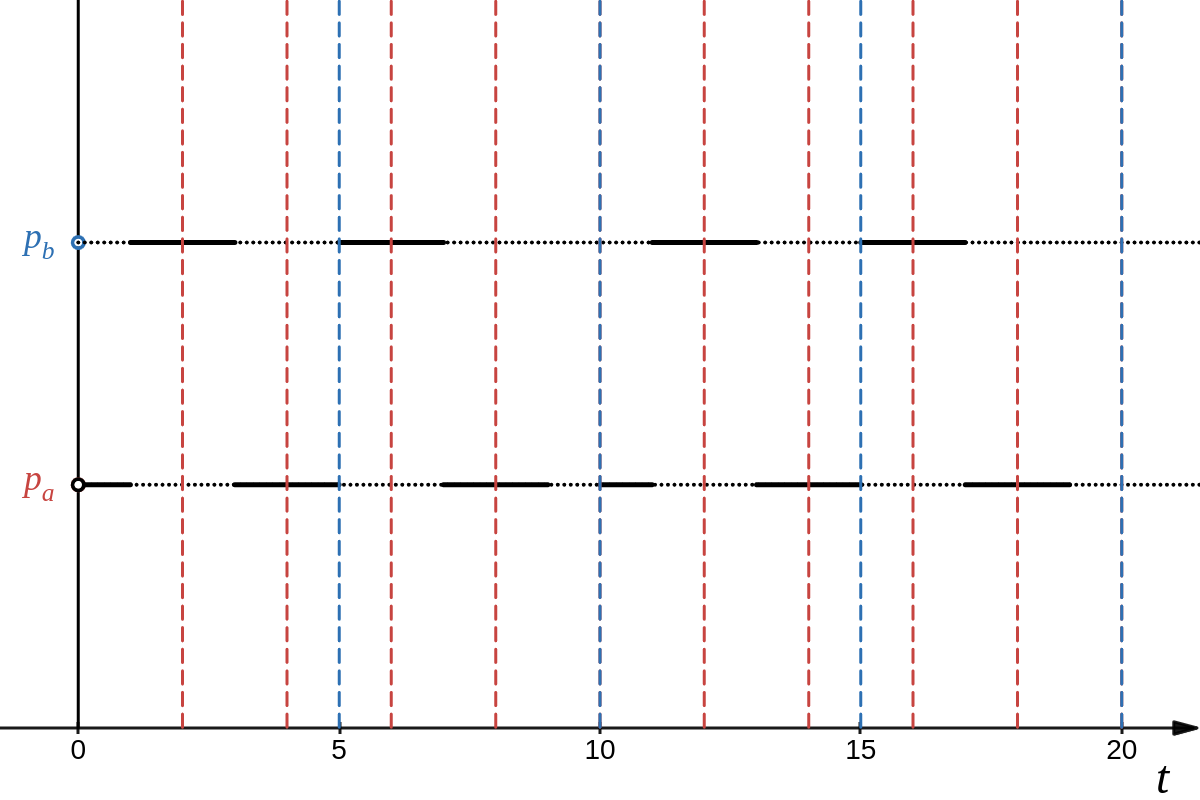
\includegraphics[scale=0.3]{../figures/rm_tight.png}
\end{center}

Vediamo quindi come siamo arrivati al 90\% di utilizzo della CPU, e come  il fatto che l'algoritmo è non preemptive significa che quando $p_b$ accede alla CPU, la tiene anche oltre la linea di periodo di $p_a$ (che ha comunque tempo di eseguire prima della linea successiva).

\subsubsection{Algoritmo RM "preemptive"}
Potremmo introdurre la preemption nell'algoritmo RM.
In questo caso, ad ogni periodo riportiamo in esecuzione il processo con priorità più alta.

\par\smallskip

Vediamo quindi la timeline che otteniamo applicando questa versione con preemption all'esempio della scorsa sezione: 
\begin{center}
	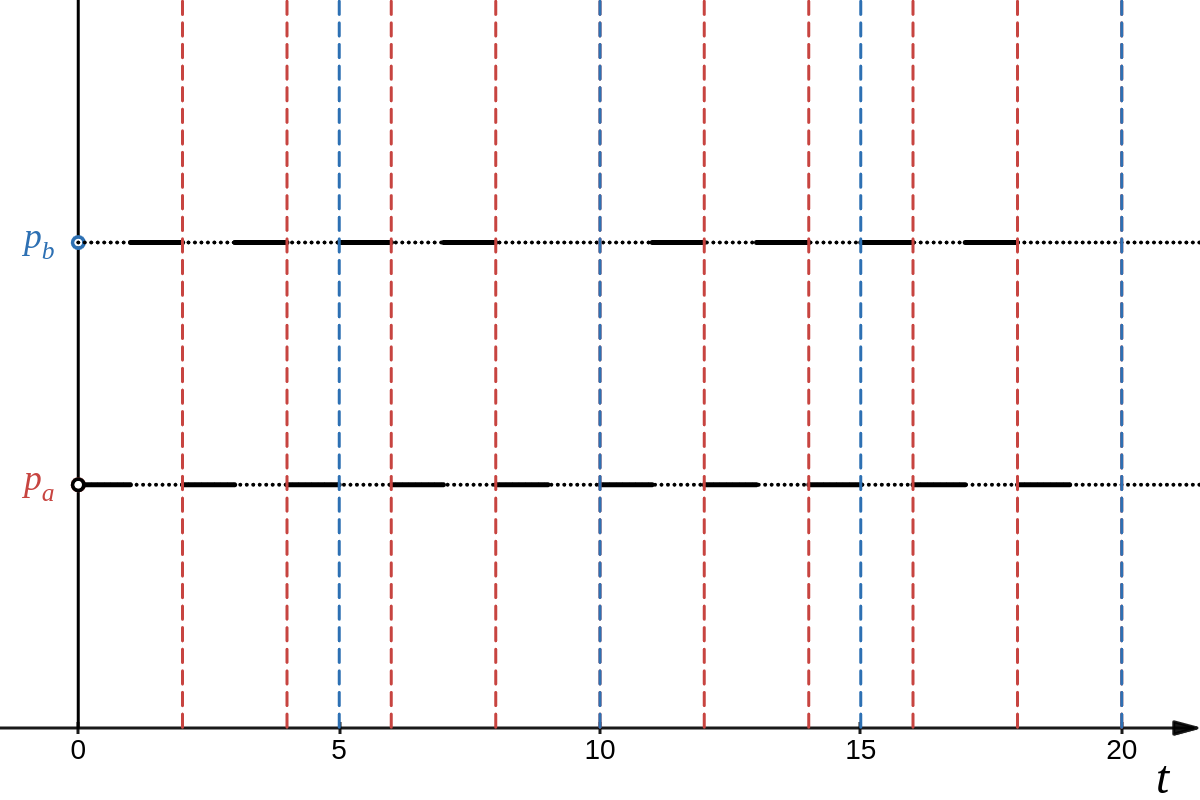
\includegraphics[scale=0.3]{../figures/rm_pre.png}
\end{center}

\par\smallskip

Notiamo che questo algoritmo di scheduling introduce un overhead maggiore della versione non preemptive, dato dai maggiori cambi di contesto. Inoltre, almeno in questo caso, non varia particolarmente in utilizzo CPU o in efficacia generale.

Comunque, possiamo osservare che mantiene i processi ancora più lontani dalla deadline, che è generalmente un comportamento desiderabile. 

\par\smallskip

Abbiamo quindi che per gli algoritmi a priorità \textit{static}, il RM è ottimo: se un insieme di processi è schedulabile a priorità statica in real-time, allora lo è con RM.
Di contro, se non è schedulabile con RM, non esiste nessun algoritmo a priorità statica che può schedularlo.

\subsection{Processi non schedulabili staticamente}
Approfondiamo cosa significa, per un insieme di processi, essere \textit{schedulabili a priorita statica}.
Prendiamo la tabella di processi: 
\begin{table}[H]
	\center \rowcolors{2}{white}{black!10}
	\begin{tabular} { c || c | c }
		\bfseries Processo & \bfseries $\Delta \mathbf{t}$ periodo & \bfseries $\mathbf{C}$ esecuzione \\
		\hline
		$p_a$ & 4 & 2 \\ 
		$p_b$ & 10 & 5
	\end{tabular}
\end{table}

Vediamo come ogni processo chiede di eseguire per metà del suo periodo.

Se usiamo la schedulazione RM in questo caso, otteniamo:
\begin{center}
	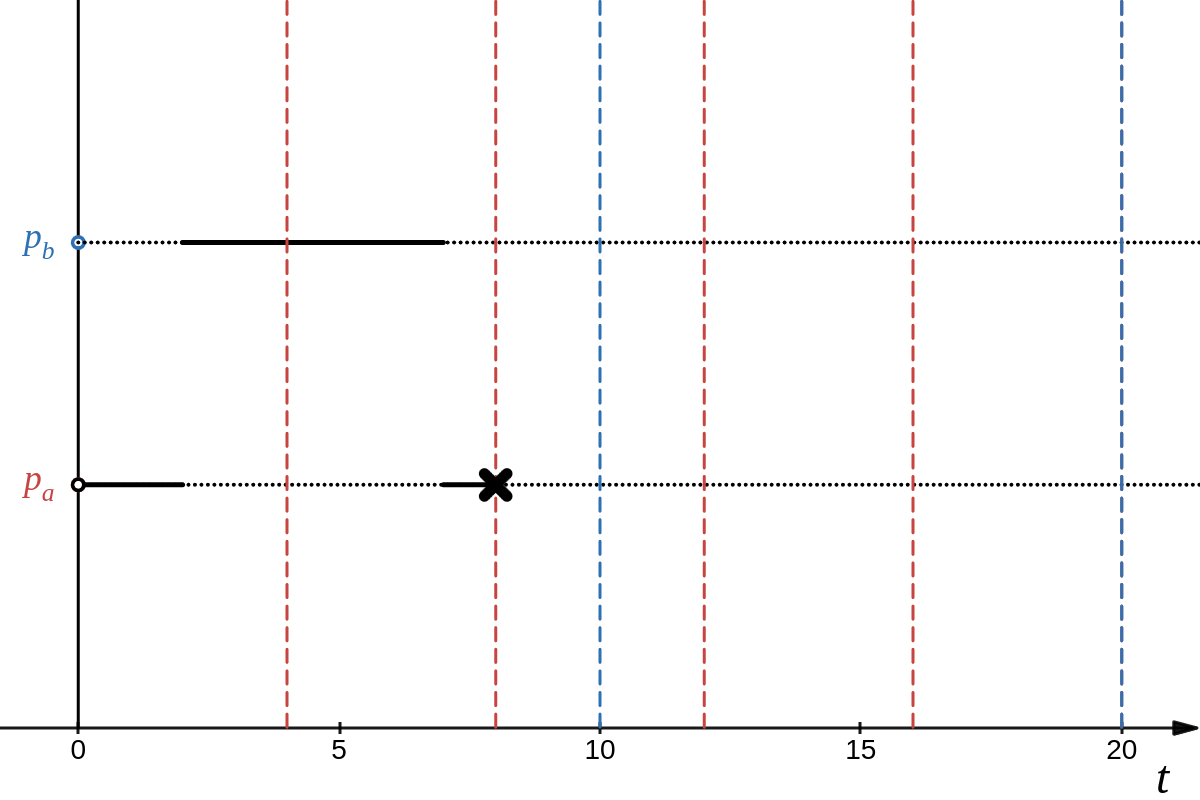
\includegraphics[scale=0.3]{../figures/rm_fail.png}
\end{center}

Dove all'istante $t = 8$ non siamo riusciti a completare il CPU burst di $p_a$, e si è quindi giunti ad un \textit{overflow}: un fallimento della schedulazione che non ha rispettato la deadline.

\newpage

Pensiamo allora di utilizzare l'algoritmo RM "preemptive" visto nella scorsa szione. In questo caso, si avrà:
\begin{center}
	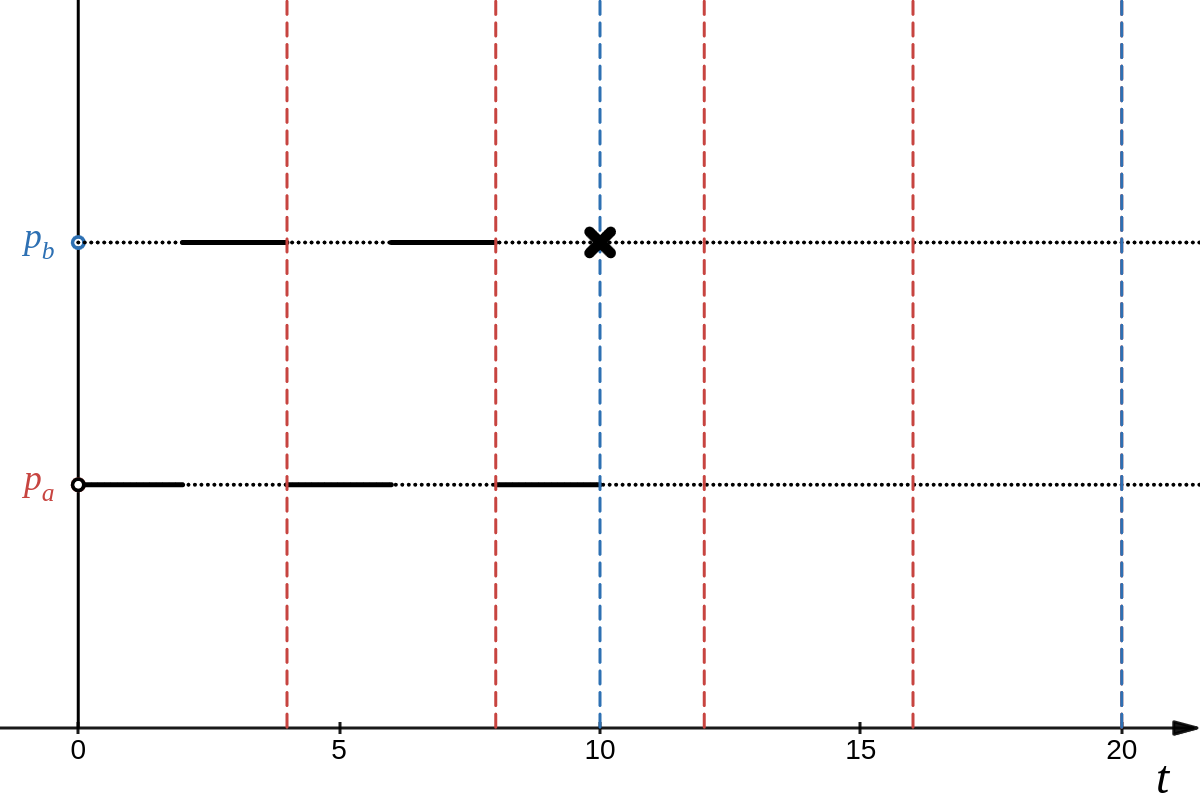
\includegraphics[scale=0.3]{../figures/rm_pre_fail.png}
\end{center}

A questo punto è $p_b$ ad andare in overflow! All'istante $t = 10$ infatti non siamo riusciti a completare le sue 5 unità temporali per completare l'esecuzione.

Abbiamo chiaramente incontrato un insieme di processi non schedulabili con priorità statica, e nemmeno introducendo la preemption abbiamo risolto il problema: dovremo trovare una qualche altra soluzione.

\subsubsection{Trattazione matematica}
Abbiamo che, nel caso dei due processi $p_a$ e $p_b$, il minimo che dobbiamo rispettare per poter in primo luogo eseguire i processi nel periodo di sistema è:
$$
n_a C_a + n_b C_b \leq T
$$
dove ricordiamo $T$ è il m.c.m. fra i periodi $t_a$ e $t_b$, e $n_a$ e $n_b$ sno rispettivamente il numero di volte in cui i processi $p_a$ e $p_b$ entrano in esecuzione per periodo di sistema.
In particolare, questi valori si possono calcolare dai perodi dei processi $\Delta t_a$, $\Delta t_b$, come:
$$
n_a = \frac{T}{\Delta t_a}, \quad n_b = \frac{T}{\Delta t_b}
$$

Sostituendo, si ha quindi:
$$
\frac{T}{\Delta t_a} C_a + \frac{T}{\Delta t_b} C_b \leq T \implies
\frac{C_a}{\Delta t_a} + \frac{C_b}{\Delta t_b} \leq 1
$$

Possiamo quindi generalizzare quanto trovato alla (ovvia) legge:
$$
U = \sum_{i = 0}^{n - 1} \frac{C_i}{T_i} \leq 1
$$
per $n$ processi arbitrari, dove $U$ viene detto \textbf{fattore di utilizzazione}.

Nell'esempio considerato finora, questo valore è:
$$
U = \frac{2}{4} + \frac{5}{10} = 1
$$
per cui i processi sono schedulabili. Ci manca da trovare un algoritmo che li sappia schedulare. 

\subsection{Algoritmo EDF}
L'algoritmo \textbf{EDF} (\textit{Earliest Deadline First}) è un algoritmo di schedulazione real-time, preemptive e a priorità dinamica.

Consiste nel mandare in esecuzione il processo che è più vicino alla sua deadline.
Come in tutti gli algoritmi a priorità dinamica, lo scheduler viene messo in esecuzione al cambio dei criteri di scelta (quindi quando un processo entra in coda pronti). In ogni caso, se due processi so trovano ugualmente vicini alla deadline al momento dell'esecuzione dello scheduler, si opta per ridurre i cambi di contesto al minimo e mantenere in esecuzione quello che sta già eseguendo.

\par\smallskip

Vediamo come questo algoritmo si applica all'esempio schedulabile visto finora:
\begin{center}
	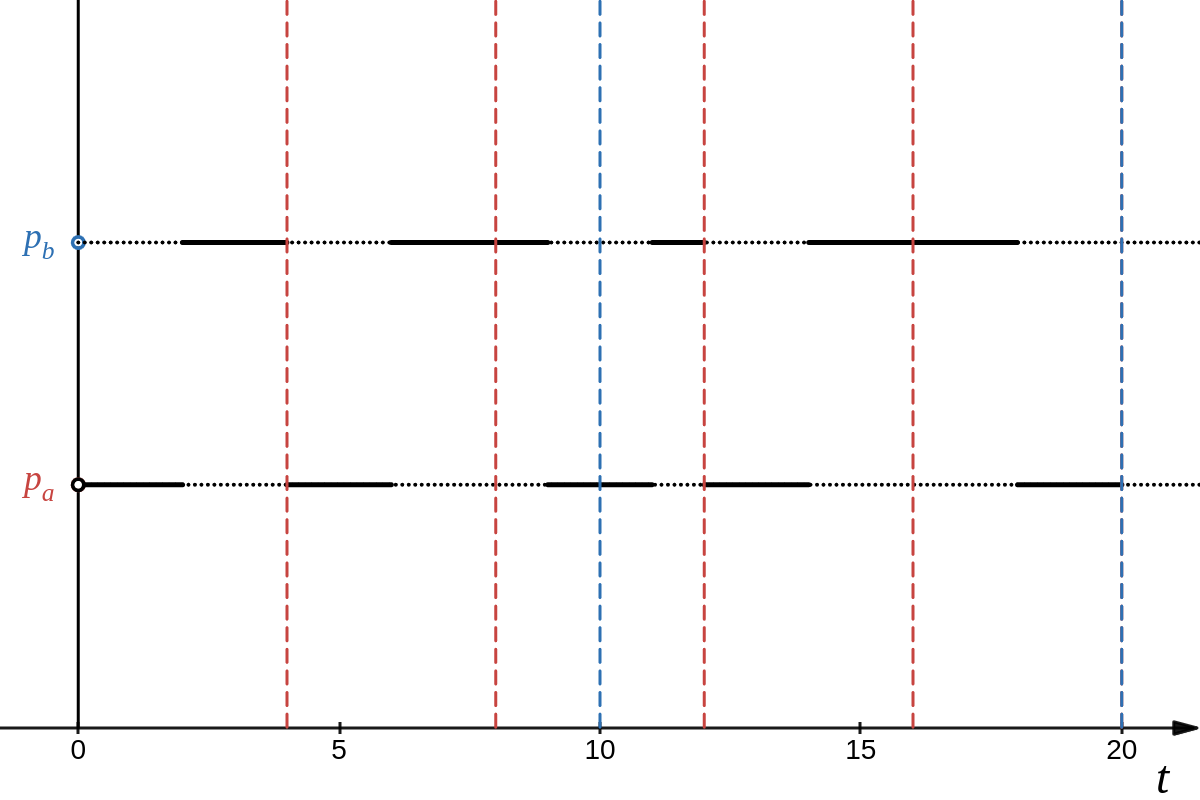
\includegraphics[scale=0.3]{../figures/edf.png}
\end{center}

Vediamo come otteniamo il 100\% dell'utilizzazione CPU, e riusciamo a schedulare i processi senza overflow.

All'istante $t = 8$, infatti, il processo $p_b$ è più vicino di $p_a$ alla deadline, e quindi viene mantenuto in esecuzione (fino a $t = 9$ dove termina).
In questo modo si riesce ad evitare che il suo CPU burst venga \textit{"tagliato"} prima che esso possa rispettare la sua deadline.

\par\smallskip

Abbiamo quindi trovato un'algoritmo che risolve i problemi che avevamo incontrato con RM: possiamo anticipare che questo algoritmo è ottimo fra gli algoritmi di schedulazione in real-time a priorità dinamica.

Una considerazione può essere fatta sull'overhead che introduciamo, almeno per l'esempio sopra. Abbiamo detto che sì, si cerca di mantenere al minimo i cambi di contesto, ma c'è comunque un certo overhead dato dall'esecuzione dello scheduler ad ogni creazione di processo.

In questo, potremmo aggiornare il modello introdotto in 9.1.1 come segue:
$$
U = ... \leq 1 - O_v 
$$
dove $O_v$ è un fattore temporale che tiene conto dell'overhead.

\subsection{Thread}
Introduciamo semplicemente il concetto di \textbf{thread} (o \textit{processo leggero}).
Avevamo detto che un processo è al contempo:
\begin{itemize}
	\item Un elemento che possiede delle \textit{risorse};
	\item Un elemento a cui viene \textit{assegnata} la CPU (si conserva lo \textit{stato} e si usa uno \textit{scheduler} per decidere quando caricarlo).
\end{itemize}

Possiamo separare questi due aspetti:
\begin{itemize}
	\item Definiamo \textbf{processo leggero}, o \textit{thread}, l'elemento a cui viene assegnata la CPU;
	\item Di contro, definiamo \textbf{processo pesante}, o \textit{task}, l'elemento che possiede le risorse.
\end{itemize}

Un processo pesante può essere composto da più thread, ognuno dei quali rappresenta effettivamente un flusso di esecuzione a sé stante. Tutti i thread possono però accedere alle risorse del loro processo pesante (incluso \textit{spazio di indirizzamento}, file aperti, ecc...). 

\end{document}

\documentclass[a4paper,11pt]{article}
\usepackage[a4paper, margin=8em]{geometry}

% usa i pacchetti per la scrittura in italiano
\usepackage[french,italian]{babel}
\usepackage[T1]{fontenc}
\usepackage[utf8]{inputenc}
\frenchspacing 

% usa i pacchetti per la formattazione matematica
\usepackage{amsmath, amssymb, amsthm, amsfonts}

% usa altri pacchetti
\usepackage{gensymb}
\usepackage{hyperref}
\usepackage{standalone}

\usepackage{colortbl}

\usepackage{xstring}
\usepackage{karnaugh-map}

% imposta il titolo
\title{Appunti Sistemi Operativi}
\author{Luca Seggiani}
\date{2025}

% imposta lo stile
% usa helvetica
\usepackage[scaled]{helvet}
% usa palatino
\usepackage{palatino}
% usa un font monospazio guardabile
\usepackage{lmodern}

\renewcommand{\rmdefault}{ppl}
\renewcommand{\sfdefault}{phv}
\renewcommand{\ttdefault}{lmtt}

% circuiti
\usepackage{circuitikz}
\usetikzlibrary{babel}

% testo cerchiato
\newcommand*\circled[1]{\tikz[baseline=(char.base)]{
            \node[shape=circle,draw,inner sep=2pt] (char) {#1};}}

% disponi il titolo
\makeatletter
\renewcommand{\maketitle} {
	\begin{center} 
		\begin{minipage}[t]{.8\textwidth}
			\textsf{\huge\bfseries \@title} 
		\end{minipage}%
		\begin{minipage}[t]{.2\textwidth}
			\raggedleft \vspace{-1.65em}
			\textsf{\small \@author} \vfill
			\textsf{\small \@date}
		\end{minipage}
		\par
	\end{center}

	\thispagestyle{empty}
	\pagestyle{fancy}
}
\makeatother

% disponi teoremi
\usepackage{tcolorbox}
\newtcolorbox[auto counter, number within=section]{theorem}[2][]{%
	colback=blue!10, 
	colframe=blue!40!black, 
	sharp corners=northwest,
	fonttitle=\sffamily\bfseries, 
	title=Teorema~\thetcbcounter: #2, 
	#1
}

% disponi definizioni
\newtcolorbox[auto counter, number within=section]{definition}[2][]{%
	colback=red!10,
	colframe=red!40!black,
	sharp corners=northwest,
	fonttitle=\sffamily\bfseries,
	title=Definizione~\thetcbcounter: #2,
	#1
}

% disponi codice
\usepackage{listings}
\usepackage[table]{xcolor}

\definecolor{codegreen}{rgb}{0,0.6,0}
\definecolor{codegray}{rgb}{0.5,0.5,0.5}
\definecolor{codepurple}{rgb}{0.58,0,0.82}
\definecolor{backcolour}{rgb}{0.95,0.95,0.92}

\lstdefinestyle{codestyle}{
		backgroundcolor=\color{black!5}, 
		commentstyle=\color{codegreen},
		keywordstyle=\bfseries\color{magenta},
		numberstyle=\sffamily\tiny\color{black!60},
		stringstyle=\color{green!50!black},
		basicstyle=\ttfamily\footnotesize,
		breakatwhitespace=false,         
		breaklines=true,                 
		captionpos=b,                    
		keepspaces=true,                 
		numbers=left,                    
		numbersep=5pt,                  
		showspaces=false,                
		showstringspaces=false,
		showtabs=false,                  
		tabsize=2
}

\lstdefinestyle{shellstyle}{
		backgroundcolor=\color{black!5}, 
		basicstyle=\ttfamily\footnotesize\color{black}, 
		commentstyle=\color{black}, 
		keywordstyle=\color{black},
		numberstyle=\color{black!5},
		stringstyle=\color{black}, 
		showspaces=false,
		showstringspaces=false, 
		showtabs=false, 
		tabsize=2, 
		numbers=none, 
		breaklines=true
}


\lstdefinelanguage{assembler}{ 
  keywords={AAA, AAD, AAM, AAS, ADC, ADCB, ADCW, ADCL, ADD, ADDB, ADDW, ADDL, AND, ANDB, ANDW, ANDL,
        ARPL, BOUND, BSF, BSFL, BSFW, BSR, BSRL, BSRW, BSWAP, BT, BTC, BTCB, BTCW, BTCL, BTR, 
        BTRB, BTRW, BTRL, BTS, BTSB, BTSW, BTSL, CALL, CBW, CDQ, CLC, CLD, CLI, CLTS, CMC, CMP,
        CMPB, CMPW, CMPL, CMPS, CMPSB, CMPSD, CMPSW, CMPXCHG, CMPXCHGB, CMPXCHGW, CMPXCHGL,
        CMPXCHG8B, CPUID, CWDE, DAA, DAS, DEC, DECB, DECW, DECL, DIV, DIVB, DIVW, DIVL, ENTER,
        HLT, IDIV, IDIVB, IDIVW, IDIVL, IMUL, IMULB, IMULW, IMULL, IN, INB, INW, INL, INC, INCB,
        INCW, INCL, INS, INSB, INSD, INSW, INT, INT3, INTO, INVD, INVLPG, IRET, IRETD, JA, JAE,
        JB, JBE, JC, JCXZ, JE, JECXZ, JG, JGE, JL, JLE, JMP, JNA, JNAE, JNB, JNBE, JNC, JNE, JNG,
        JNGE, JNL, JNLE, JNO, JNP, JNS, JNZ, JO, JP, JPE, JPO, JS, JZ, LAHF, LAR, LCALL, LDS,
        LEA, LEAVE, LES, LFS, LGDT, LGS, LIDT, LMSW, LOCK, LODSB, LODSD, LODSW, LOOP, LOOPE,
        LOOPNE, LSL, LSS, LTR, MOV, MOVB, MOVW, MOVL, MOVSB, MOVSD, MOVSW, MOVSX, MOVSXB,
        MOVSXW, MOVSXL, MOVZX, MOVZXB, MOVZXW, MOVZXL, MUL, MULB, MULW, MULL, NEG, NEGB, NEGW,
        NEGL, NOP, NOT, NOTB, NOTW, NOTL, OR, ORB, ORW, ORL, OUT, OUTB, OUTW, OUTL, OUTSB, OUTSD,
        OUTSW, POP, POPL, POPW, POPB, POPA, POPAD, POPF, POPFD, PUSH, PUSHL, PUSHW, PUSHB, PUSHA, 
				PUSHAD, PUSHF, PUSHFD, RCL, RCLB, RCLW, MOVSL, MOVSB, MOVSW, STOSL, STOSB, STOSW, LODSB, LODSW,
				LODSL, INSB, INSW, INSL, OUTSB, OUTSL, OUTSW
        RCLL, RCR, RCRB, RCRW, RCRL, RDMSR, RDPMC, RDTSC, REP, REPE, REPNE, RET, ROL, ROLB, ROLW,
        ROLL, ROR, RORB, RORW, RORL, SAHF, SAL, SALB, SALW, SALL, SAR, SARB, SARW, SARL, SBB,
        SBBB, SBBW, SBBL, SCASB, SCASD, SCASW, SETA, SETAE, SETB, SETBE, SETC, SETE, SETG, SETGE,
        SETL, SETLE, SETNA, SETNAE, SETNB, SETNBE, SETNC, SETNE, SETNG, SETNGE, SETNL, SETNLE,
        SETNO, SETNP, SETNS, SETNZ, SETO, SETP, SETPE, SETPO, SETS, SETZ, SGDT, SHL, SHLB, SHLW,
        SHLL, SHLD, SHR, SHRB, SHRW, SHRL, SHRD, SIDT, SLDT, SMSW, STC, STD, STI, STOSB, STOSD,
        STOSW, STR, SUB, SUBB, SUBW, SUBL, TEST, TESTB, TESTW, TESTL, VERR, VERW, WAIT, WBINVD,
        XADD, XADDB, XADDW, XADDL, XCHG, XCHGB, XCHGW, XCHGL, XLAT, XLATB, XOR, XORB, XORW, XORL},
  keywordstyle=\color{blue}\bfseries,
  ndkeywordstyle=\color{darkgray}\bfseries,
  identifierstyle=\color{black},
  sensitive=false,
  comment=[l]{\#},
  morecomment=[s]{/*}{*/},
  commentstyle=\color{purple}\ttfamily,
  stringstyle=\color{red}\ttfamily,
  morestring=[b]',
  morestring=[b]"
}

\lstset{language=assembler, style=codestyle}

% disponi sezioni
\usepackage{titlesec}

\titleformat{\section}
	{\sffamily\Large\bfseries} 
	{\thesection}{1em}{} 
\titleformat{\subsection}
	{\sffamily\large\bfseries}   
	{\thesubsection}{1em}{} 
\titleformat{\subsubsection}
	{\sffamily\normalsize\bfseries} 
	{\thesubsubsection}{1em}{}

% tikz
\usepackage{tikz}

% float
\usepackage{float}

% grafici
\usepackage{pgfplots}
\pgfplotsset{width=10cm,compat=1.9}

% disponi alberi
\usepackage{forest}

\forestset{
	rectstyle/.style={
		for tree={rectangle,draw,font=\large\sffamily}
	},
	roundstyle/.style={
		for tree={circle,draw,font=\large}
	}
}

% disponi algoritmi
\usepackage{algorithm}
\usepackage{algorithmic}
\makeatletter
\renewcommand{\ALG@name}{Algoritmo}
\makeatother

% disponi numeri di pagina
\usepackage{fancyhdr}
\fancyhf{} 
\fancyfoot[L]{\sffamily{\thepage}}

\makeatletter
\fancyhead[L]{\raisebox{1ex}[0pt][0pt]{\sffamily{\@title \ \@date}}} 
\fancyhead[R]{\raisebox{1ex}[0pt][0pt]{\sffamily{\@author}}}
\makeatother

\begin{document}
% sezione (data)
\section{Lezione del 21-10-25}

% stili pagina
\thispagestyle{empty}
\pagestyle{fancy}

% testo
\subsection{Tassonomia di Flynn}
Prima di venire alla sincronizzazione dei processi, vediamo brevemente la \textbf{classificazione delle architetture} attraverso la \textit{tassonomia di Flynn}.

Questa è una classificazione che vede un sistema di elaborazione da 2 punti di vista ortogonali:
\begin{itemize}
	\item La capacità di avere più flussi di \textbf{esecuzione}: si possono distinguere \textbf{SI} (\textit{Single Instruction Stream}) e \textbf{MI} (\textit{Multiple Instruction Stream}). Questo concetto è vicino a quello di \textit{thread} visto nella scorsa sezione;
	\item La capacità di avere più flussi di \textbf{dati}: si possono distinguere \textbf{SD} (\textit{Single Data Stream}) e \textbf{MD} (\textit{Multiple Data Stream});
\end{itemize}

Abbiamo quindi la prima distinzione:
\begin{table}[H]
	\center \rowcolors{2}{white}{black!10}
	\begin{tabular} { p{3.5cm} || c | c  }
		& \bfseries SI (\textit{Single Instruction Stream}) & \bfseries MI (\textit{Multiple Instruction Stream}) \\
		\hline\hline
		\bfseries SD (\textit{Single Data Stream}) & Macchine SISD & Macchine MISD \\
		\bfseries MD (\textit{Multiple Data Stream}) & Macchine SIMD & Macchine MIMD \\
	\end{tabular}
\end{table}

Iniziamo a vedere dove si collocano le macchine che conosciamo.

\subsubsection{Macchine SISD}
Le macchine SISD rappresentano le tradizionali macchine \textit{sequenziali} e \textit{monoprocessore} definite dall'architettura di Von Neumann.
In questo caso si ha un solo flusso di istruzioni, ciascuna agente su al più un flusso dati, e ad ogni istante temporale si esegue una singola istruzione.

Vediamo una schematizzazione di questa architettura coerente con Flynn:
\begin{center}
	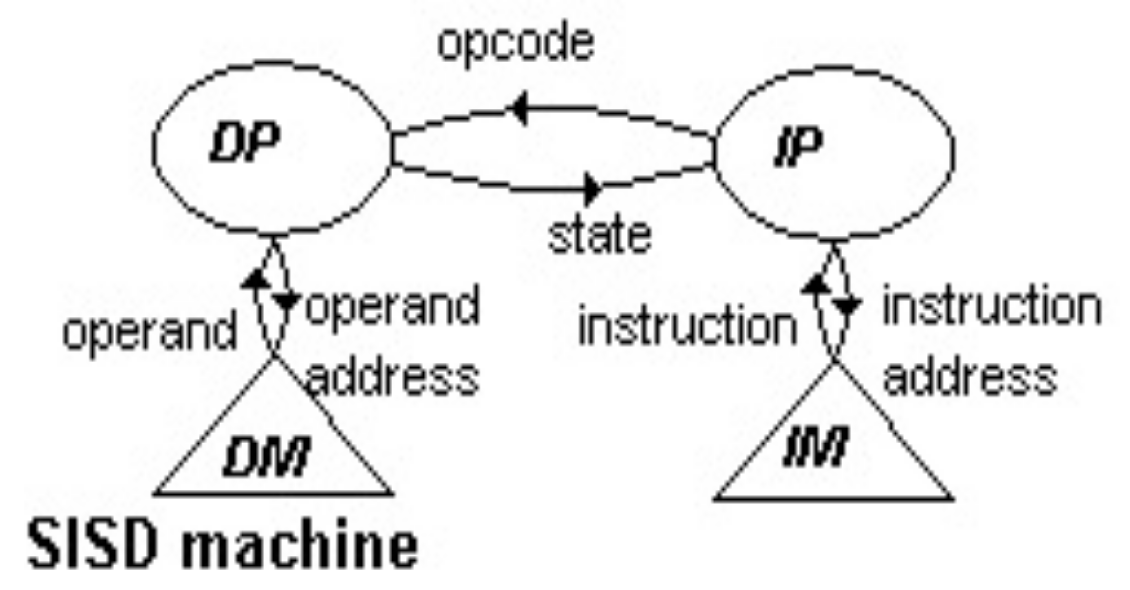
\includegraphics[scale=0.2]{../figures/sisd_flynn.png}
\end{center}

Da questa schematizzazione notiamo:
\begin{itemize}
	\item Un'unita di elaborazione \textbf{dati}, detta \textbf{DP} (\textit{Data Processor}), che interagisce ottenendo operandi e fornendo indirizzi di operandi (e sperabilmente dati) con uno stream \textbf{dati}, detto \textbf{DM} (\textit{Data Memory});
	\item Un'unità di elaborazione \textbf{istruzioni}, detta \textbf{IP} (\textit{Instruction Processor}), che interagisce ottenendo istruzioni e fornendo indirizzi di operazioni con uno stream \textbf{istruzioni}, detto \textbf{IM} (\textit{Instruction Memory}).
\end{itemize}

IP e DP interagiscono scambiandosi codifiche di istruzioni (IP $\rightarrow$ DP) e variazioni di stato (della memoria dati, DP $\rightarrow$ IP). 

Possiamo notare che la cosiddetta \textit{architettura Harvard} è un architettura che prevede, come dalla schematizzazione sopra, una forte separazione fra stream istruzioni e dati (di contro alla Von Neumann, che prevede un unica fonte di memoria per dati e istruzioni). 
Entrambe le architetture sono classificate come SISD, la Harvard è più usata in sistemi real-time mentre la Von Neumann è ancora oggi più usata nei sistemi general purpose.

\subsubsection{Macchine SIMD}
Le macchine SIMD sono formate da unità di elaborazione multiple, che eseguono le stesse istruzioni \textit{contemporaneamente}, ma su flussi di dati differenti.

\newpage

Una schematizzazione simile a quella sopra riportata è la seguente:
\begin{center}
	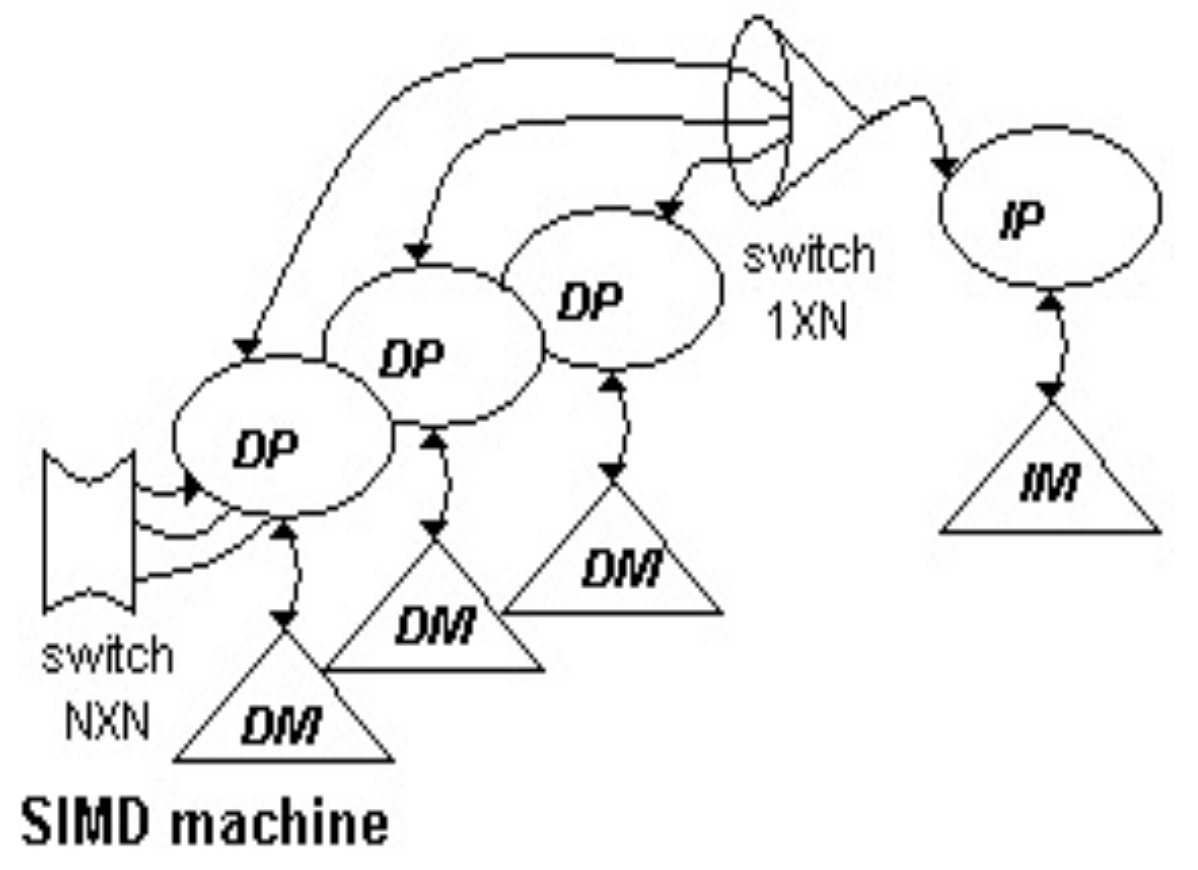
\includegraphics[scale=0.2]{../figures/simd_flynn.png}
\end{center}

Abbiamo che questa moltiplicazione dei flussi dati su cui si elabora si ha moltiplicando le unità di elaborazione dati (i \textbf{DP}), facendole obbedire ad una singola unità di elaborazione istruzion (l'\textbf{IP}).
Vediamo innanzitutto come si realizza la sincronizzazione fra questi DP: si prevede uno \textit{switch} $1\times N$ che porta le codifiche di istruzioni dall'IP a tutti i DP.

Per l'interazione fra le DP prevediamo poi uno switch $N \times N$ che le collega. Chiaramente questo switch sarà inefficiente, e vorremo usarlo il meno possibile.

Architetture di questo tipo possono essere \textit{regolari} o create \textit{ad hoc} sulla base della struttura del problema: nel caso di architetture regolari (cioè che rispettano la topologia fisica) non si hanno conflitti, e questo le rende efficienti e poco costose.

Le applicazioni di un'architettura di questo tipo sono nel caso di operazioni fortemente vettorizzate, come ad esempio nelle applicazioni grafiche e multimediali.
Inoltre, questo è il tipo di architettura che incontriamo spesso per macchine che devono portare avanti moli massiccie di computazione come i \textit{supercomputer}.

\par\smallskip

Riassumendo, possiamo dire che l'architettura SIMD prevede 2 tipi di parallelismo:
\begin{itemize}
	\item \textbf{Parallelismo temporale}: c'è un meccanismo di \textit{pipeline}, cioè fasi diverse di un’unica istruzione sono eseguite in parallelo in differenti moduli connessi in cascata.
	\item \textbf{Parallelismo spaziale}: i medesimi passi sono eseguiti contemporaneamente su un array di processori perfettamente uguali, sincronizzati da un solo controllore.
\end{itemize}

\par\smallskip

Lato programmatore possiamo prevedere due paradigmi per la compilazione di programmi pensati per l'esecuzione su macchine SIMD:
\begin{itemize}
	\item Il primo modo è non riscrivere il codice, sapendo che un programma pensato come scalare su macchina sequenziale (SISD), in esecuzione su macchina SIMD sarà vettoriale.

Avremo quindi che, ad esempio:
\begin{lstlisting}[language=C++, style=codestyle]	
// somma scalari
c = a + b
\end{lstlisting}
su macchina SIMD diventerà:
\begin{lstlisting}[language=C++, style=codestyle]	
// soma vettori (!)
C = A + B
\end{lstlisting}

	\item Nel caso si voglia essere più espliciti nel tipo di operazioni che facciamo, possiamo implementare un \textbf{compilatore vettoriale}: l'idea è che questo riconosca automaticamente quando le istruzioni SIMD potrebbero tornare utili per parallelizzare delle operazioni vettoriale, e inserisca quindi le operazioni necessarie.

		Ad esempio, potremmo volere:
\begin{lstlisting}[language=C++, style=codestyle]	
for(int i = 0; i < 100; i++) {
		c[i] = a[i] + b[i];
}
// qui riconosciamo che il ciclo e' vettorizzabile, e quindi lo vettorizziamo
\end{lstlisting}
\end{itemize}

\subsubsection{Macchine MISD}
In una macchina MISD vogliamo avere più flussi di istruzioni che lavorano contemporaneamente su un unico flusso dati.

Abbiamo che questa categoria è sostanzialmente vuota: il parallelismo fra più istruzioni in esecuzione sullo stesso flusso dati si ha effettivamente nei processori moderni solo attraverso il meccanismo della \textbf{pipeline}.

Se prevediamo che il processore debba svolgere per ogni istruzione più fasi, fra cui ad esempio:
\begin{enumerate}
	\item Prelievo istruzione;
	\item Decodifica;
	\item Prelievo operandi;
	\item Esecuzione;
	\item Scrittura.
\end{enumerate}
Avremo che questo potrà, disponendo di più unità di elaborazione atte a completare ognuna di queste fasi, parallelizzare come segue:
\begin{center}
	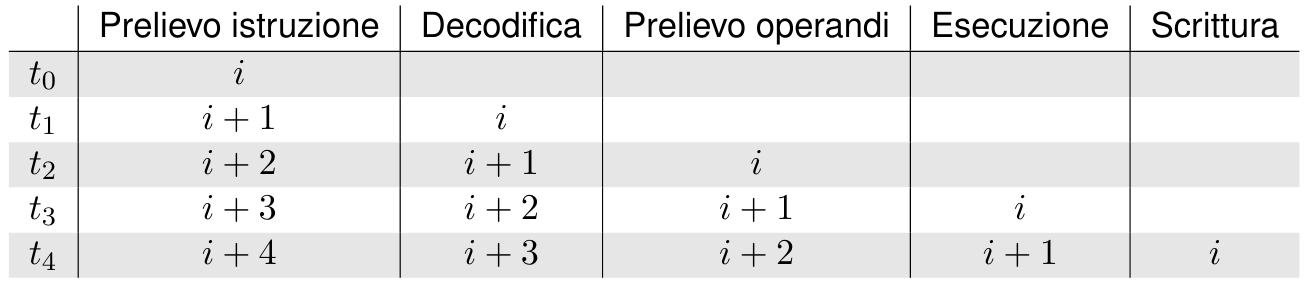
\includegraphics[scale=0.3]{../figures/pipeline.png}
\end{center}

In questo, a regime (nella tabella tempo $t_4$) si avranno più di un unità di elaborazione a lavoro contemporaneamente, e potremmo dire di aver realizzato in qualche modo il paradigma MISD.

Facciamo tra l'altro una nota sull'efficienza: se l'esecuzione di un'istruzione senza pipeline richiedeva un tempo $\Delta t$, e il troughput era $\frac{1}{T}$, prevedendo una pipeline ad $n$ stadi si riesce ad arrivare a $\frac{1}{T} \times n$ (assunto che ogni stadio richieda lo stesso tempo e si riesca a ridurre l'overhead dato da $n$ troppo grandi).

\subsubsection{Macchine MIMD}
Le macchine MIMD rappresentano per noi la categoria più interessante più flussi di istruzioni sono in esecuzione contemporaneamente su più processori, elaborando insiemi di dati distinti, privati o condivisi.

Ne prevediamo due tipologie principali:
\begin{itemize}
	\item \textbf{DM-MIMD} (\textit{Distributed Memory MIMD}), cioè a \textit{memoria distribuita}. Queste si schematizzano come segue:
\begin{center}
	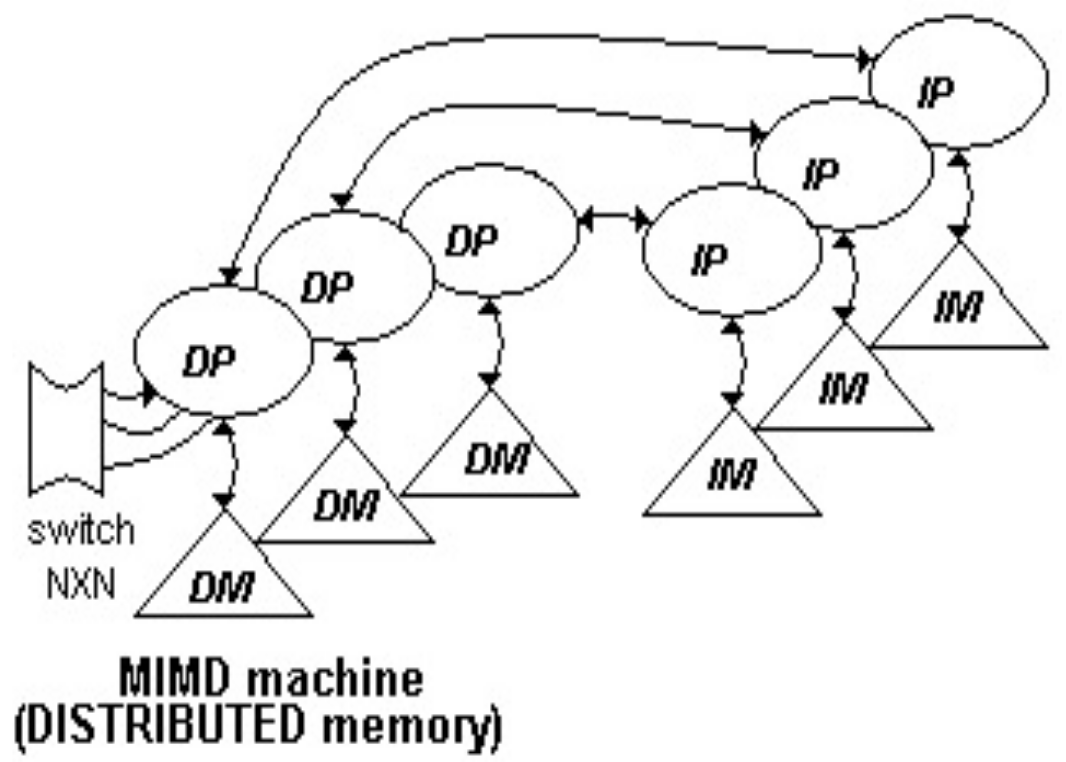
\includegraphics[scale=0.2]{../figures/dm-mimd.png}
\end{center}

In questo caso abbiamo più coppie IP-DP (con relative memorie IM e DM), che rappresentano sostanzialmente più macchine SISD. Uno switch $N \times N$ permette quindi la comunicazione fra le unità.

Abbiamo quindi che tra i nodi non esiste memoria condivisa e ogni nodo esegue indipendentemente un flusso di istruzioni su un differente insieme di dati, memorizzati su spazi differenti. La comunicazione è realizzata mediante una sottorete dedicata (appunto, lo switch).

Applicazioni di questa architettura sono ad esempio una qualsiasi \textit{rete di calcolatori} (come sia sviluppato lo switch non è specificato dal modello, e per noi potrebbe essere anche un router internet). 
Questo è il caso dei \textit{cluster} di workstation, realizzati solitamente attraverso \textit{Ethernet}. In questo richiediamo dalle macchine che compongono la rete 2 caratteristiche principali:
\begin{enumerate}
	\item \textbf{High-availability}: in caso di guasti, la computazione può migrare da un nodo all’altro;
	\item \textbf{Load-balancing}: i task da eseguire sono allocati nei nodi che hanno il minor carico.
\end{enumerate}

Architetture MIMD più stabili sono poi le rete di interconnessione regolari e dirette (ipercubi, mesh, torus), attraverso cui i nodi si scambiano informazioni secondo il paradigma del \textit{message passing} (\textit{"scambio di messaggi"}). Queste macchine sono molto scalabili e si prestano bene ad algoritmi ad elevata località: sono stati costruiti cluster composti anche da milioni di unità sequenziali.

\par\smallskip

Una variante del DM-MIMD è il \textbf{DM-MIMD MPP} (\textit{Massively Parallel Processing}). Questo è un paradigma utile in applicazioni scientifiche e particolari contesti di calcolo commerciale-finanziario. In un sistema MPP si ha:
\begin{itemize}
	\item Migliaia di nodi (CPU standard, ognuna con la propria memoria e la propria copia del SO)
	\item Una rete di interconnessione custom molto potente (larga banda e bassa latenza). Affinché l’elaborazione MPP dia effettivi vantaggi occorre disporre di software capace di partizionare il lavoro e i dati su cui opera tra i vari processori.
\end{itemize}

\item \textbf{SM-MIMD} (\textit{Single Memory MIMD}), cioè a \textit{memoria condivisa}. Queste si schematizzano come segue:
\begin{center}
	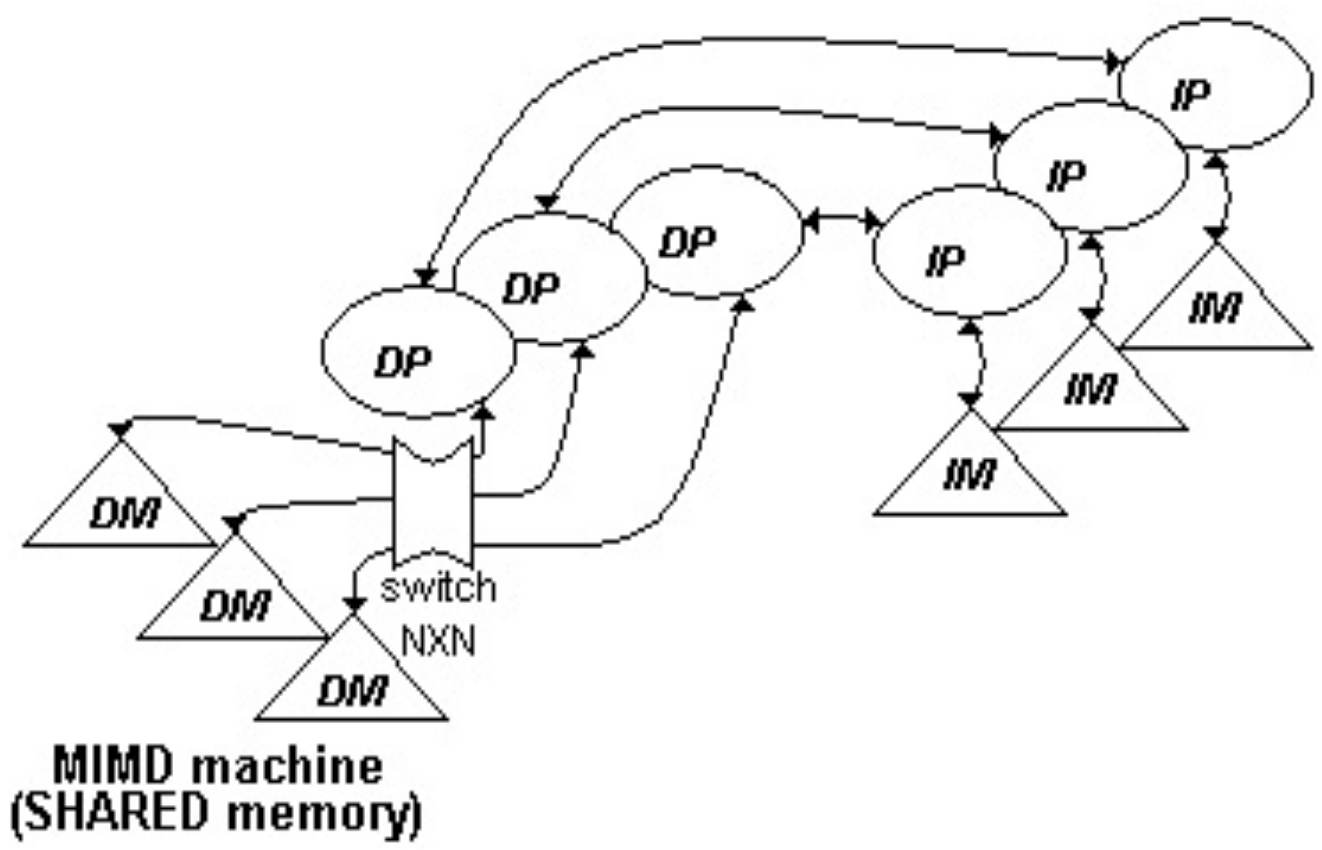
\includegraphics[scale=0.2]{../figures/sm-mimd.png}
\end{center}

Sono quindi macchine sempre \textit{multiprocessore}, ma dove le varie unità di elaborazione dati comunicano attraverso uno switch $N \times N$ con un \textit{pool} unico di memoria (formato anche da più flussi di memoria, ma visti allo stesso modo da ogni unità di elaborazione dati).

Questo approccio è meno scalabile, realizza la comunicazione fra processori condividendo aree di memoria, e richiede una rete di interconnessione (lo switch $N \times N$ estremamente efficiente).
Vogliamo che il numero $N$ di processori sia piccolo ($N < 100$), affiché si possa avere stretto accompiamento fra i nodi.
Si incorre chiaramente in problemi di competizione fra unità di elaborazione (mutua esclusione e sincronizzazione) che potrebbero impattare le prestazioni.
\end{itemize}

\subsubsection{Confronto fra SIMD e MIMD}
Possiamo fare quindi un confronto fra le architetture apperentemente simili, SIMD e MIMD:
\begin{itemize}
	\item Le SIMD richiedono meno hardware delle MIMD (c'è un unica unità di controllo, o \textit{elaborazione istruzioni});
	\item Le MIMD usano spesso processori general-purpose, quindi costano meno delle SIMD (che richiedono processori o ISA particolari, quindi meno hardware ma più specializzato);
	\item Le SIMD usano meno memoria delle MIMD (una sola copia del programma in memoria);
	\item Le MIMD godono di una grande flessibilità in termini di modelli computazionali supportati (si pensi \textit{client-server}, \textit{P2P}, ecc...). Di contro, è piuttosto semplice modificare un programma seqeunziale perché esegua su architettura SIMD in maniera vettorizzata.
\end{itemize}

\subsubsection{Sintesi della tassonomia di Flynn}
Possiamo quindi vedere un grafico riassuntivo delle tassonomie viste:
\begin{center}
	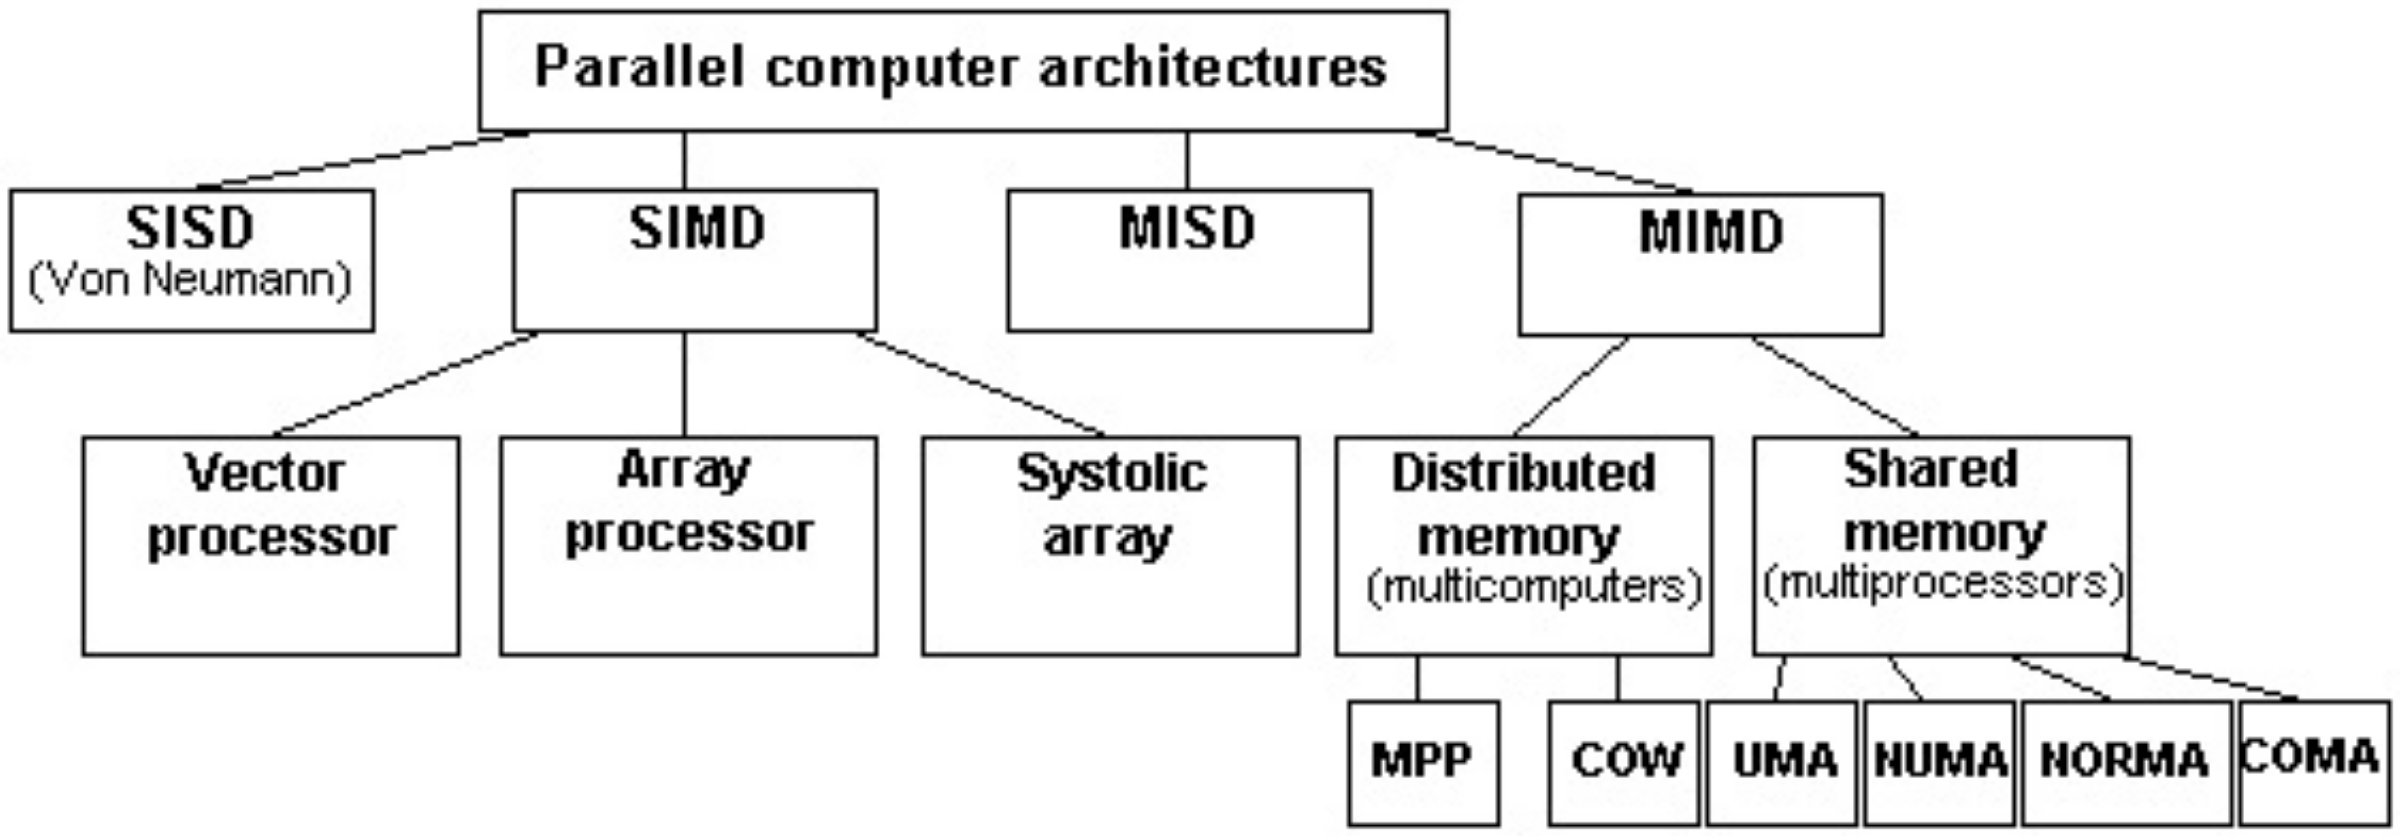
\includegraphics[scale=0.17]{../figures/flynn.png}
\end{center}

Dove si notano le 4 categorie principali (SISD, SIMD, MISD e MIMD) ed alcune sottocategorie (non abbiamo parlato di tutte le sottocategorie, per una trattazione più completa si rimanda alla letteratura).

\subsection{Tipologie di interconnessione}
Dopo aver discusso le architetture descritte dalla tassonomia di Flynn, vediamo i tipi principali di \textbf{interconnessione} che si possono avere fra unità di elaborazione (o in generale nodi).

\subsubsection{Bus}
\begin{center}
	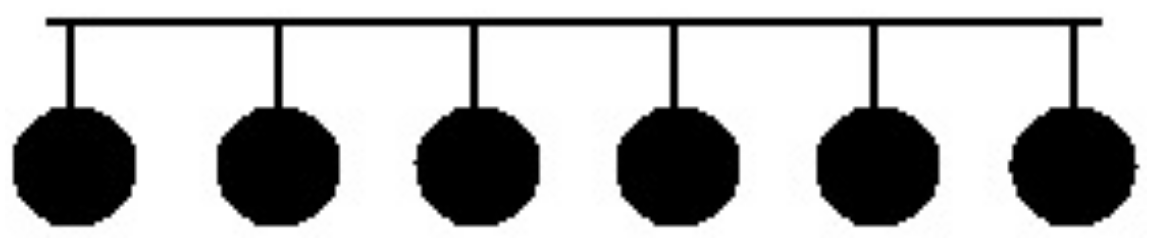
\includegraphics[scale=0.11]{../figures/bus.png}
\end{center}
Il \textbf{bus} è la più semplice rete di interconnessione che abbiamo visto.
Rappresenta una configurazione semplice ed affidabile (a meno che non si rompa il bus tutto funziona), dove ogni nodo a \textit{grado} 1 (tutti i nodi sono direttamente connessi al bus e a nient'altro), e il \textit{diametro} è 1 (la distanza massima è data dal solo bus).
Il numero totale di \textit{link} di cui abbiamo bisogno è sempre 1: il bus stesso è l'unico link di cui necessitiamo (i nodi devono solo collegarsi a tale link).

Il problema è chiaramente la \textit{competizione} sull'accesso al mezzo, che è massima: si hanno spesso problemi di mutua esclusione sulle stesse risorse, ad esempio quando più nodi vogliono accedere alla stessa risorsa contemporaneamente e devono farlo attraverso un unico bus.

\newpage

\subsubsection{Array lineare}
\begin{center}
	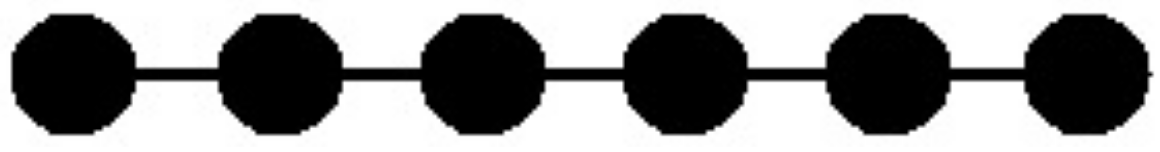
\includegraphics[scale=0.11]{../figures/linear.png}
\end{center}
L'\textbf{array lineare} espande in qualche modo l'idea del bus: in un certo senso vogliamo partizionare il bus in tanti link nodo a nodo. In questo caso il grado del primo e dell'ultimo nodo sarà 1, mentre quello dei restanti nodi sarà 2. Il diametro sara $n - 1$ per $n$ nodi, e il numero totale di link $n - 1$ (quelli necessari a legare ogni nodo con i nodi adiacenti).

Il vantaggio di questo approccio è la competizione, che viene ridotta al minimo (ogni coppia adiacente di nodi può comunicare indipendentemente dagli altri). Più nello specifico, nel caso ideale possiamo avere fino a $\frac{N}{2}$ competizioni contemporanee e parallele (appunto, una per ogni coppia).

I nodi dovranno quindi fornire servizi di \textit{routing}, cioè permettere a nodi da un capo dell'array di comunicare con nodi dall'altro capo, prendendosi a carico in qualche modo il messaggio da comunicare.
Questo è chiaramente a scapito della robustezza: se un nodo si rompe due parti dell'array lineare rimangono separate.

\subsubsection{Ring}
\begin{center}
	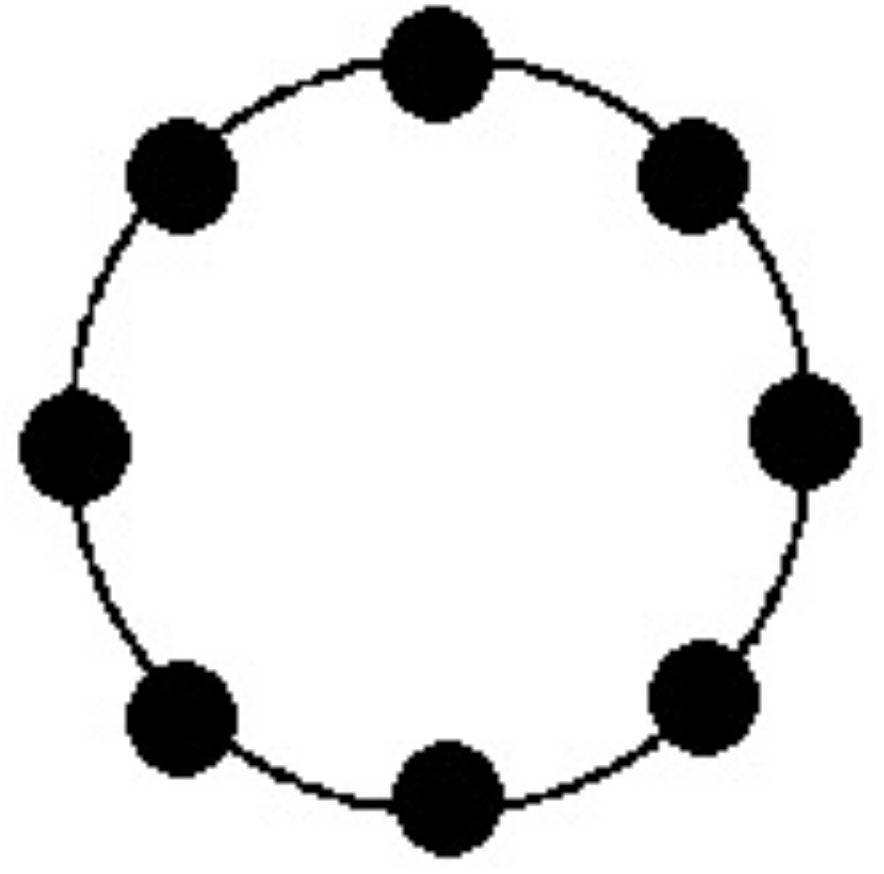
\includegraphics[scale=0.11]{../figures/ring.png}
\end{center}
Il \textbf{ring} è un array lineare chiuso su stesso (dove si sono collegati i nodi estremi, cioè quelli con grado 1). Il grado diventa quindi 2 per tutti i nodi. 
Il diametro subisce la prima caratteristica fondamentale del ring: per raggiungere un dato nodo si hanno a disposizione due direzioni anziché una, per cui il diametro complessivo è $\frac{N}{2}$.

Anche la tolleranza ai guasti migliora, in quanto un nodo guasto non pregiudica necesssariamente l'integrità del sistema (ne servono 2 per isolare una parte della rete).

\subsubsection{Connessione completa}
\begin{center}
	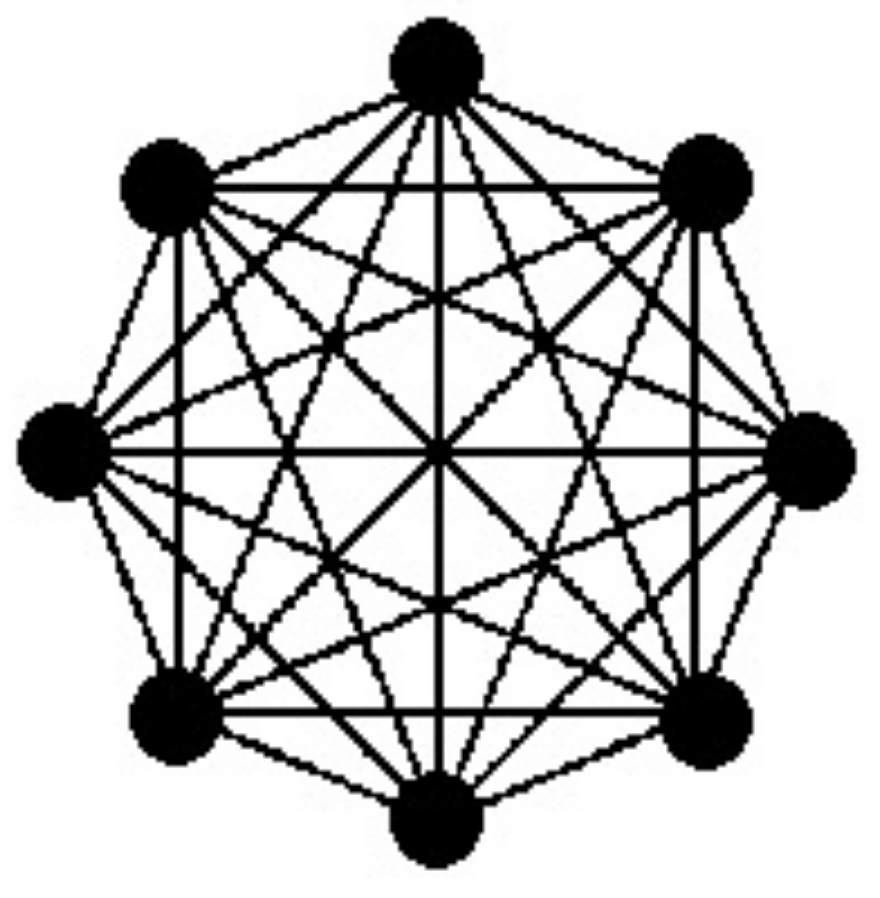
\includegraphics[scale=0.12]{../figures/full_conn.png}
\end{center}
La \textbf{connessione completa} (o \textit{tutti-a-tutti}) è la rete di interconnessione più, appunto, \textit{connessa}, che vediamo.
In questo caso ogni nodo comunica direttamente con ogni altro nodo: il grado è per tutti i nodi $N - 1$ e il diametro è 1 (si arriva direttamente al nodo desiderato).
Svantaggioso è chiaramente il numero totale di link, che cresce come $N \frac{N - 1}{2}$: l'approccio chiaramente non è scalabile!

Dobbiamo quindi trovare modelli per reti di interconnessione che presentino parte dei vantaggi della connessione completa (alta tolleranza ai guasti, bassissimo diametro), riducendo però il numero di link e quindi aumentando la scalabilità.

\subsubsection{Albero binario}
\begin{center}
	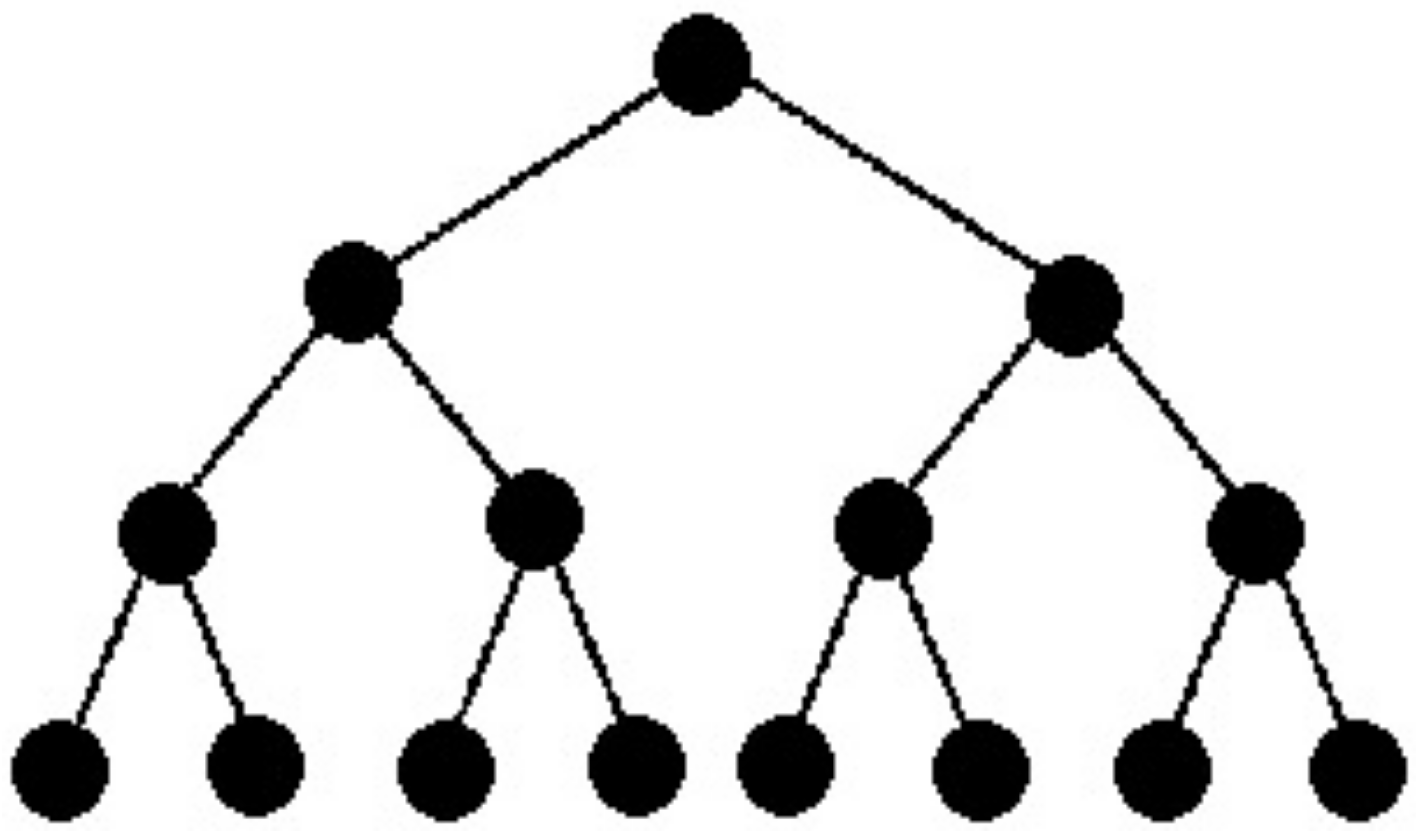
\includegraphics[scale=0.11]{../figures/btree.png}
\end{center}
Si può pensare di ordinare i nodi secondo un \textbf{albero binario}.
In questo caso vorremo definire l'\textit{altezza} dell'albero come $h = \log_2(N)$ per $N$ nodi e i gradi come:
\begin{itemize}
	\item 2 per la radice;
	\item 1 per le foglie;
	\item 3 per tutti gli altri nodi.
\end{itemize}
Il diametro sarà (senza dimostrazione) $2 \times (h - 1)$ e il numero totale di link $N - 1$ ($O(N)$ anziché $O(N^2)$, già migliore).

Questo tipo di rete permette una facile comunicazione fra nodi sugli stessi sottoalberi, mentre per comunicazioni fra sottoalberi distinti porta alla \textit{congestione dei rami alti}: questo la rende poco scalabile.
In particolare, più ci avviciniamo alla radice minori saranno i link (e quindi maggiore il carico sul singolo link). Inoltre, i nodi dovranno fare da router, e quindi più ci avviciniamo alla radice più i nodi hanno responsabilità di router sempre maggiori.
Questo culmina sulla radice stessa, che chiaramente è sottoposta ad un carico non indifferente e rappresenta il punto più debole dell'architettura ad albero binario.

Per quanto riguarda la tolleranza ai guasti, vale lo stesso discorso: più in alto (verso la radice) avviene il guasto, maggiori sono le conseguenze per il sistema. Come caso limite, se si guasta la radice si incorre in un partizionamento in due dell'intero sistema.

Soluzioni alternative si possono avere sfruttando alberi, anziche binari, \textit{$n$-ari}, cioè con $n$ figli per nodo.

\subsubsection{Stella}
\begin{center}
	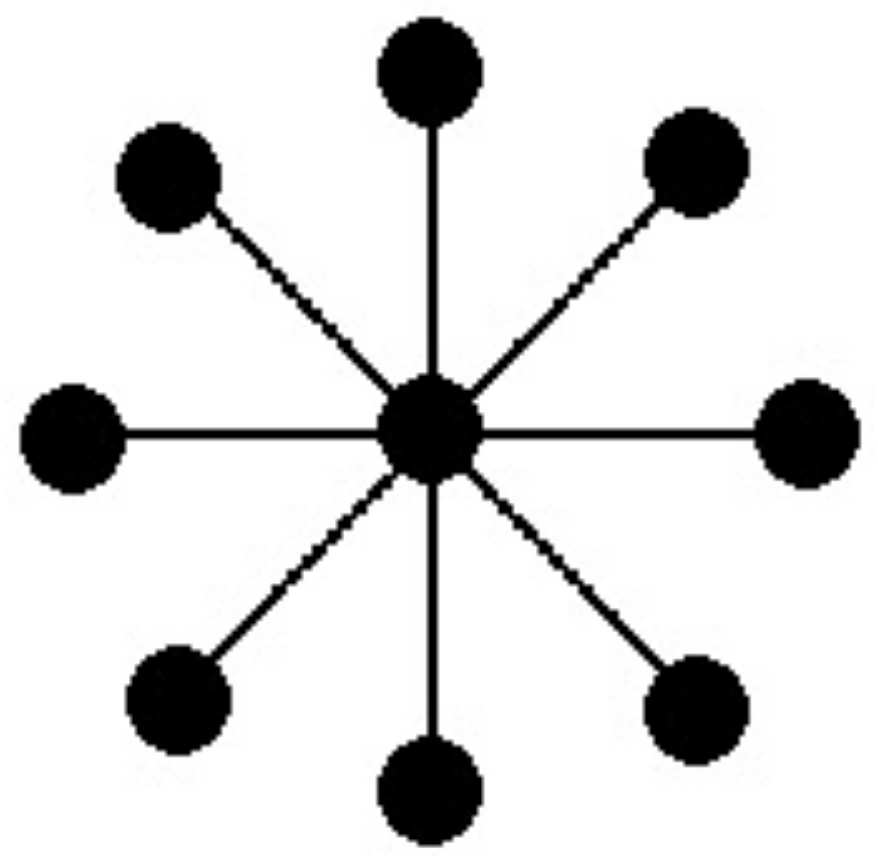
\includegraphics[scale=0.11]{../figures/star.png}
\end{center}
Le reti di interconnessione a \textbf{stella} prevedono un singolo nodo centrale che connette $n-1$ nodi periferici.
Il grado di tale nodo centrale sarà quindi $n - 1$, mentre i nodi periferici avranno 1.
Il diametro sarà 2 (dobbiamo passare sempre dal nodo centrale, a meno che non si voglia parlare col nodo centrale stesso).
Il numero di link è ridotto ($N - 1$), e quindi da questo punto di vista il sistema è vantaggioso.

Il difetto più grande è chiaramente la presenza di un singolo nodo centralizzato soggetto a guasti o sovraccarichi.
Questo è il classico problema del \textit{single point of failure} delle architetture client-server: possiamo infatti intendere il nodo centrale come un \textit{server} e i nodi periferici come \textit{client} di tale server.

Abbiamo quindi che per quanto si possa rendere potente il nodo server, questo dovrà portare tutto il carico della rete (bassa scalabilità), e un guasto del server rappresenterà una mancanza di servizio per tutti i nodi client (bassa robustezza).

\subsubsection{Mesh bidimensionale}
\begin{center}
	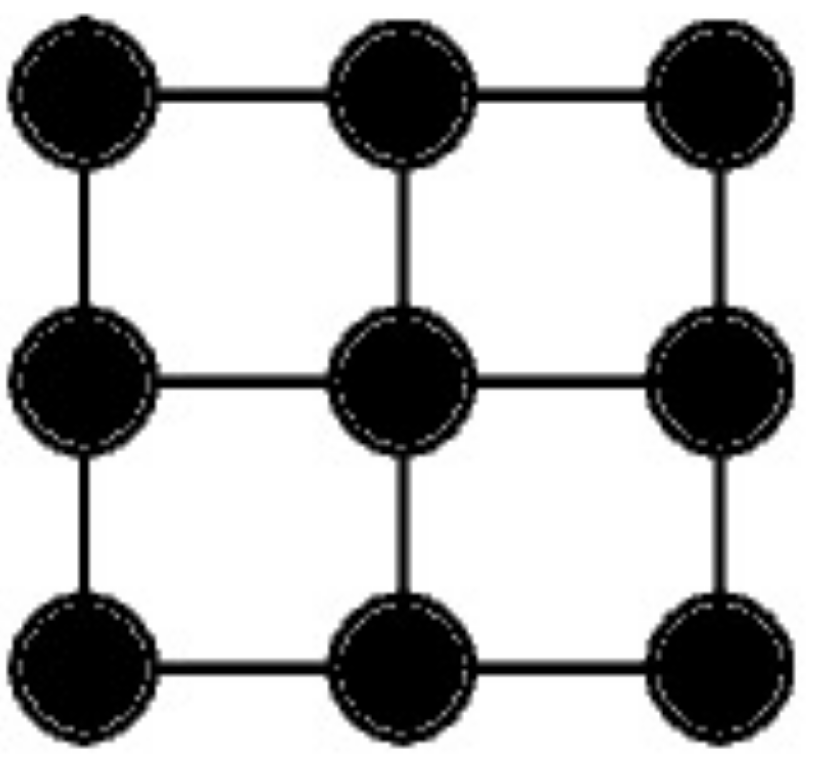
\includegraphics[scale=0.09]{../figures/mesh.png}
\end{center}
La struttura a \textbf{mesh bidimensionale} prevede di disporre i nodi su una griglia bidimensionale.
In questo caso il lato della griglia sarà $r = \sqrt{N}$ e il grado dei nodi sarà:
\begin{itemize}
	\item 2 per i nodi ai vertici,
	\item 3 per in nodi \textit{"centrali"} ai lati (diciamo nodi agli \textit{spigoli});
	\item 4 per tutti gli altri nodi.
\end{itemize}
Il diametro sarà $2 \times (r - 1)$, e il numero totale di link ($2 \times (n - 2) \times r$).

La resistenza ai guasti di queste configurazioni è buona, ma può essere milgiorata. Vediamo come.

\subsubsection{Toro bidimensionale}
\begin{center}
	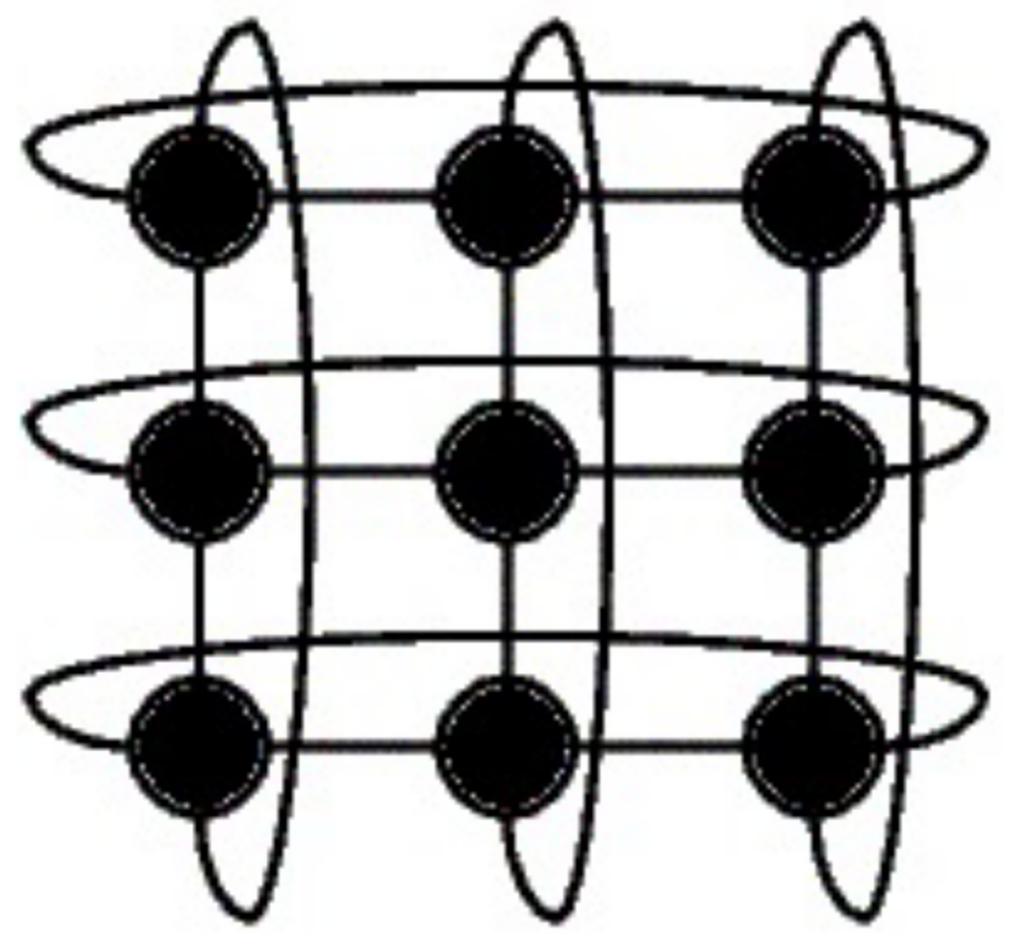
\includegraphics[scale=0.1]{../figures/torus.png}
\end{center}
Collegando i nodi ai lati opposti di una struttura a mesh bidimensionale si ottiene una struttura a \textbf{toro bidimensionale}.
In questo caso il grado è 4 per tutti i nodi, ma il diametro migliora: va sostanzialemente come $r$ (dove $r$ è il lato calcolato come $r = \sqrt{N}$, uguale alla rete bidimensionale).
Il numero totale di link è invece stabile a $2N$.

Questa topologia risulta ben scalabile e notevolmente resistente ai guasti: sostanzialmente rappresenta per la mesh bidimensionale quello che il ring rappresenta per l'array lineare.

\par\medskip

Architetture come le ultime viste (mesh, tori, ecc...) possono essere estese a più dimensioni, portando a \textit{ipercubi}, \textit{ipertori}, ecc... 

\subsection{Metriche di prestazione}
Finiamo questa sezione del programma parlando di alcune \textbf{metriche} per le \textbf{prestazioni} di architetture descritte secondo la tassonomia di Flynn.

\begin{itemize}
	\item Chiamiamo \textbf{speed-up} ($S$) il rapporto fra il tempo di esecuzione sequenziale sul tempo di esecuzione parallelo (SIMD o MIMD, cioè):
		$$
			S = \frac{T_1}{T_N}
		$$

		Questa metrica rappresenta quindi il \textit{guadagno} in velocità che si ha passando ad un sistema multiprocessore. Idealmente vorremmo $S = N$, cioè \textit{lineare} col numero di unità di elaborazione, ma come vedremo a causa dell'overhead introdotto da più processori dobbiamo accontentarci di $S < N$, con $S \approx N$.

		l valore dello speed-up dipende dalle applicazioni, ma anche dall’architettura: nelle SIMD spesso $S \approx N$, mentre nelle MIMD è difficile far crescere $S$ (non è facile far lavorare pienamente tutte le CPU, o trasferire efficientemente fra di esse).

	\item L'\textbf{efficienza} ($E$) è invece definita come lo speed-up sul numero di unità di elaborazione, cioè:
		$$
			E = \frac{S}{N}
		$$
		Come prima, vorremmo $E = 1$, ma dobbiamo accontentarci di $E < 1$, con $E \approx 1$.
\end{itemize}

Per giustificare come mai non si può mai avere $S = N$ (o equivalentemente, $E = 1$), ci viene incontro la \textit{legge di Amdhal}.
Questa dice che un parallelismo \textit{"perfetto"} (nelle varie attività compiute da un calcolatore) non è mai raggiungibile in quanto saranno \textit{sempre} presenti sequenza di programmi \textit{intrinsecamente seriali}.
Semplificando, si può dire che ci saranno sempre degli intervalli di tempo sequenziale ($T_\text{seq}$), impiegati ad eseguire istruzioni non parallelizzabili come operazioni di I/O, costrutti condizionali, algoritmi intrinsecamente sequenziali, ecc....

Più nello specifico, la legge di Amdahl ridefinisce lo speed-up come:
$$
S = \frac{T_1}{T_{\text{seq}} + \frac{T_1 - T_\text{seq}}{N} }
$$
cioè il guadagno di speed-up è dato solo dalle parti parallelizzabili del programma ($T_1 - T_\text{seq}$), mentre le parti seriali ($T_\text{seq}$) non hanno grandi guadagni.

Il problema è che, prendendo il limite per $N \rightarrow \infty$, si ha:
$$
\lim_{N \rightarrow \infty} S = \lim_{N \rightarrow \infty} \frac{T_1}{T_{\text{seq}} + \frac{T_1 - T_\text{seq}}{N} } = \frac{T_1}{T_\text{seq}}
$$
cioè a dominare lo speed-up sono le parti sequenziali (le parti non sequenziali vengono abbattute velocemente, quelle sequenziali mai e rimangono come overhead complessivo dell'intero sistema).

\subsubsection{Multitasking}

In conclusione, vogliamo dire che il \textit{multitasking} è quasi sempre vantaggioso (anche intuitivamente), ed è di notevole importanza anche nelle macchine per mantere alto lo sfruttamento delle CPU (ciò che avevamo chiamato \textit{efficienza CPU}).

Il vincolo che vogliamo rispettare sarà, quindi, di base:
$$
P >> N
$$
cioè avere più processi che unità di elaborazione. 

\subsection{Sincronizzazione processi}
Iniziamo quindi a vedere la \textbf{sincronizzazione} fra processi, in particolare con riferimento ai \textit{tipi} di interazione che ci possono essere fra processi, e i problemi di \textbf{mutua esclusione} e \textbf{sincronizzazione}.

\subsubsection{Tipi di interazione}
Ricordiamo che i processi possono interagire fra di loro secondo 2 modalità:
\begin{itemize}
	\item \textbf{Cooperazione}: quindi per sincronizzazione diretta o esplicita, cioè definita dai programmi;
	\item \textbf{Competizione}: quindi per sincronizzazione indiretta o implicita, non definita dal codice dei programmi ma causata da tentativi di accesso \textit{simultaneo} a risorse limitati. 
\end{itemize}

Nominiamo poi l'\textbf{interferenza}, rappresentata da errori dipendenti dal tempo.

Per l'interazione fra processi faremo riferimento a 2 modelli principali:
\begin{itemize}
	\item A \textbf{memoria comune}: in questo caso prevediamo $n$ processi con risorse private (cioè spazi di indirizzamento privati per ognuno), ma che possono accedere a risorse \textit{condivise} in un terzo spazio di indirizzamento comune per tutti. 

		Se vogliamo ricondurci alla tassonomia di Flynn, questo è un esempio di macchina multiprocessore (o monoprocessore in \textit{timesharing}...) di tipo MIMD (se vogliamo SM-MIMD): più unità di elaborazione sugli stessi dati (tralasciando il fatto che ogni unità ha poi i suoi dati privati);

	\item A \textbf{scambio di messaggi}: in questo caso prevediamo $n$ processi in esecuzione su unità di elaborazione distinte (ancora, multiprocessore o monoprocessore in \textit{timesharing}) con le loro risorse (memorie) locali, che possono comunicare fra di loro attraverso un meccanismo di \textit{scambio di messaggi}.

Notiamo di nuovo che non è necessario che le unità siano necessariamente distinte, e ricordiamo che non sono i processi a comunicare in sé per sé, ma le unità di elaborazione a supportare un meccanismo che permette tale comunicazione.

		Questo è sempre un esempio di architettura MIMD (se vogliamo DM-MIMD), simile ad esempio a quella che ci permettono i sistemi multicalcolatore connessi in rete (più macchine distinte, con le loro risorse, che comunicano fra di loro).
\end{itemize}



\end{document}

\end{document}